\documentclass[final]{ukthesis}
%you must include these 2 packages.
\usepackage[pdfauthor={Sen Li},
            pdftitle={RGB-D Cameras’ Parallel Calibration and 3D Reconstruction in Real-Time},
            pdfsubject={3D Camera Calibration},
            pdfkeywords={3D Reconstruction; Camera Calibration; RGBD; Image Processing},
            pdfproducer={Latex with hyperref},
            pdfcreator={latex->dvips->ps2pdf},
            pdfpagemode=UseOutlines,
            bookmarksopen=true,
            letterpaper,
		hidelinks,
            bookmarksnumbered=true]{hyperref}
\usepackage{memhfixc}

\usepackage{mathptmx}% http://ctan.org/pkg/mathptmx
\usepackage{amsmath}
\usepackage{graphicx}
\usepackage[lofdepth,lotdepth]{subfig}
\usepackage{textcomp}
\usepackage{amssymb}
\usepackage{caption}
\usepackage{float}

\DisemulatePackage{setspace}
\usepackage{setspace}

\usepackage[autostyle=true]{csquotes} % Required to generate language-dependent quotes in the bibliography
\graphicspath{{Figures/}{./}} % Specifies where to look for included images

\usepackage{multirow}
\usepackage{makecell}
\usepackage{varwidth}

\usepackage{color}
\usepackage[T1]{fontenc}

\setcounter{MaxMatrixCols}{20}

%\usepackage{amsxtra}     % Use various AMS packages
%\usepackage{amssymb}
%\usepackage{amsfonts}
%\usepackage{graphicx}    % Add some packages for figures. Read epslatex.pdf on ctan.tug.org
%\usepackage{rotating}
%\usepackage{color}
%\usepackage{epsfig}
%\usepackage{verbatim}
%\usepackage{natbib}      % Allows you to use BibTeX
%\usepackage[printonlyused]{acronym} 

%%%%%%%%%%%%%%%%%%%%%%%%%%%%%%%%%%%%%%%%%%%%%%%%
\begin{document}
%author data  Electrical Engineering
\author{Sen Li}
\title{Universal Real-Time XYZ Calibrated Reconstruction\\ for RGB-D Cameras}
\abstract{%
Ever since the Kinect brought low-cost depth cameras into consumer market, with PrimeSense 3D
sensing technology as the core depth determination principle for its first generation,
great interest has been invigorated into RGB-D sensors. However, there has not been a systematic solution to combine both of 3D reconstruction and the radial dominated lens distortions correction. What is worse, the traditional pinhole-camera-model based 3D camera calibration method does not consider the depth distortion. In this thesis, a data-based look-up table software calibration method is proposed to do real-time rectified 3D reconstruction for universal RGB-D cameras. The idea is inspired and extended from a structured light real-time 3D reconstruction system. A transition from pinhole-camera calibration model to data-based lens distortion-removed calibration model is analyzed. High-order polynomial surface mapping is employed for non-linear distortion correction, and an individual Bluetooth Low Energy Optical-Flow tracking module is introduced for external \(Z^w\) value support.
}
\advisor{Dr. Daniel L. Lau}
\keywords{3D Reconstruction; Camera Calibration; RGBD; Image Processing}
\dgs{Dr. Caicheng Lu}


%the title pages
\frontmatter
%\maketitle


%\begin{acknowledgments}
%Acknowledge people/things here
%\end{acknowledgments}
%\begin{dedication}
%Dedicated to things (optional)
%\end{dedication}


\tableofcontents\clearpage
\listoffigures\clearpage
\listoftables\clearpage


%----------------------------------------------
\mainmatter

\onehalfspacing

%%% Chapter 1
\chapter{Introduction} % Main chapter title
%\label{sens_introduction} % For referencing the chapter elsewhere, use \ref{sens_introduction} 
%%%%%%%%%%%%%%%%%%%%%%%%%%%%%%%%%%%%%%%%%%%%%%%%%%
%%%%%%%%%%%                                                     %%%%%%%%%%%%%%%%%%%%%%%%%%%
%%%%%%%%%%%           1.1   Consumer RGBD Cameras                   %%%%%%%%%%%%%%%%%%%%
%%%%%%%%%%%                                                     %%%%%%%%%%%%%%%%%%%%%%%%
%%%%%%%%%%%%%%%%%%%%%%%%%%%%%%%%%%%%%%%%%%%%%%%%%%%
\section{RGBD Cameras}
\indent
A RGB-D camera, also called depth camera, is a sensing system that capture RGB images along with per-pixel depth information. Usually it is simply a combination of a RGB sensor a depth sensor with certain alignment algorithm between them. Ever since the Kinect brought low-cost depth cameras into consumer market, with PrimeSense 3D sensing technology as the core depth determination principle for its first generation, great interest has been invigorated into RGB-D sensors. As the depth sensor technologies opens a new epoch for three-dimensional (3D) markets, the multimedia technologies development is changing from two-dimensional (2D) to 3D on games, movies, health care aid, military training, \textit{etc}., all various areas that are in demand of a more direct reflection on the real world \cite{depthOverview12}. Simple 2D scenes are not able to meet the social demands any more. And with the fast development of multimedia technologies, three-dimensional scene display has become a hotspot in the display field. As an extension of classic 2D video, the 3D dynamic display technology can provide a more comprehensive immersive feeling to users than a 2D video. Gesture recognition, 3D modeling, 3D printing, augmented reality, virtual reality, \textit{etc}., a lot of ongoing researches and applications on depth cameras are famous now, cooperated with Human Computer Interaction (HCI) technologies. %
\\\indent%
The PrimeSense's technology had been originally applied to gaming, whose user interfaces are based on gesture recognition instead of using a controller (also called Natural User Interface, NUI). It was best known for licensing the hardware design and chip used in Microsoft's first generation of Kinect motion-sensing system for the Xbox 360 in 2010. The PrimeSense sensor projects an infrared speckle pattern, which will then be captured by an infrared camera in the sensor. A special microchip is employed to compare the captured speckle pattern part-by-part to reference patterns stored in the device, which were captured previously at known depths. The final per-pixel depth will be estimated based on which reference patterns the captured pattern matches best. Other than the first generation of Kinect camera, Asus Xtion PRO sensor, another consumer NUI application product, has also applied the PrimeSense's technology.
\\\indent%
As a competitor of PrimeSense Structured Light technology, time-of-flight technology had been applied into PMD[Vision] CamCube cameras and 3DV's ZCam cameras. Based on known speed of light, Time-of-Flight (ToF) camera resolves distance by measuring the \enquote{time cost} of a special light signal traveling between the camera and target for every single point. The \enquote{time cost} variable that ToF camera measures is the phase shift between the illumination and reflection, which will be translated to distance \cite{TimeOfFlight}. To detect the phase shifts, light source is pulsed or modulated by a continuous wave, typically a sinusoid or square wave. The ToF camera illumination is typically from a LED or a solid-state laser operating in the near-infrared range invisible to human eyes. Fabrizio \textit{et al}.\cite{depthTechCompare_2011} compared the time-of-flight (PMD[Vision] CamCube) camera and PrimeSense (first generation Kinect) camera in 2011. He showed that the time-of-flight technology is more accurate and claimed that the time-of-flight technology will not only be extended to support colours and higher frame sizes, but also rapidly drop in price. In 2009, 3DV agreed to sell its ZCam assets to Microsoft. And in 2013,  Microsoft released the Xbox One, whose NUI sensor KinectV2 features a wide-angle ToF camera.
\\\indent
Unlike the PrimeSense's speckle pattern or KinectV2's ToF, Intel RealSense camera utilizes stereo vision. Its sensor actually has three cameras: two IR cameras (left and right), and one RGB camera. Additionally, RealSense camera also has an IR laser projector to help the stereo vision recognize depth at unstructured surfaces. Compared with KinectV2 camera, RealSense camera is more like a desktop usage to capture faces or even finger gestures, whereas the KinectV2 could do better to capture the full body actions with all joints. The effective distances of KinectV2 and RealSense hardwares are different. The KnectV2 is optimized to 0.5m ~4.5m, while RealSense are designed for 0.2m~1.2m depends on different devices.

%%%%%%%%%%%%%%%%%%%%%%%%%%%%%%%%%%%%%%%%%%%%%%%%%%
%%%%%%%%%%%                                                                %%%%%%%%%%%%%%%%%
%%%%%%%%%%     1.2  Human Computer Interface                %%%%%%%%%%%%%%%%%%%%
%%%%%%%%%%%                                                                %%%%%%%%%%%%%%%%%%
%%%%%%%%%%%%%%%%%%%%%%%%%%%%%%%%%%%%%%%%%%%%%%%%%%%
\section{Human Computer Interface}
%%
%%
%%
%% gesture recognition
\indent
Pattern recognition and gesture recognition are of the hottest sustained research activities in the area of HCI. Being a significant part in non verbal communication hand gestures are playing vital role in our daily life. Hand Gesture recognition system provides us an innovative, natural, user friendly way of interaction with the computer which is more familiar to the human beings. Gesture Recognition has a wide area of application including human machine interaction, sign language, immersive game technology \textit{etc}. By keeping in mind the similarities of human hand shape with four fingers and one thumb, \cite{gestureRecognition12} presents a real time system for hand gesture recognition on the basis of detection of some meaningful shape based features like orientation, center of mass (centroid), status of fingers, thumb in terms of raised or folded fingers of hand and their respective location in image. Since gestures based on hand and finger movements can be robustly understood by computers by using a special 3D IR camera, users are allowed to play games and interact with computer applications in natural and immersive ways that improve the user experience. In 2010, Microsoft's first generation Kinect, using PrimeSense’s technology, is based on projecting a structured light pattern on the object in order to build and track the skeleton of the user’s body to control a series of electronic games. \cite{SL3Dfrom2D96} also discussed similar techniques for 3D object reconstruction. The appearance of RGBD cameras around revolutionized robotics applications, as the sensor is very easy to use and offers data of enough quality for most applications. By offering an alternative to time-cost procedures such as stereo-vision and laser scanning, RGB-D cameras open up the possibility of real-time robot interaction in human environments. Using this depth-map along with the 2D color images obtained via the Kinect camera, the computational unit of the Xbox 360 console was capable of providing a fairly robust gesture recognition solution. After \cite{KinectGesture12} proposed two methods for gesture recognition, a plethora of applications have been produced around Kinect by various groups of image processing researchers.
\\\indent%
\begin{figure}[t]
\centering
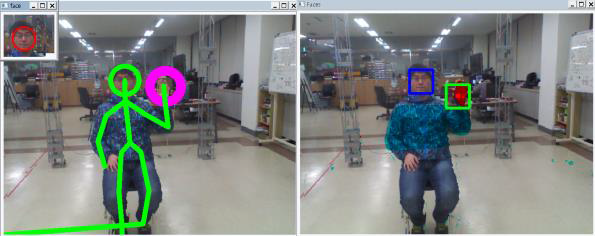
\includegraphics[width=0.65\textwidth]{KinectBasedCallingGesture}
\caption{Calling Gesture Recognition Using Kinect \cite{gestureKinect14}}
\label{KinectBasedCallingGesture}
\end{figure}%
%
A Kinect-based calling gesture recognition scenario is proposed by \cite{gestureKinect14} for taking order service of an elderly care robot. Its proposed scenarios are designed mainly for helping non expert users like elderly to call service robot for their service request. In order to facilitate elderly service, natural calling gestures are designed to interact with the robot. Fig.~\ref{KinectBasedCallingGesture} shows the evaluation of gesture recognition when sitting on chair. Individual people is segmented out from 3D point cloud acquired by Microsoft Kinect, skeleton is generated for each segment, face detection is applied to identify whether the segment is human or not, and specific natural calling gestures are designed based on skeleton joints. %
%
\begin{figure}[t]
\centering
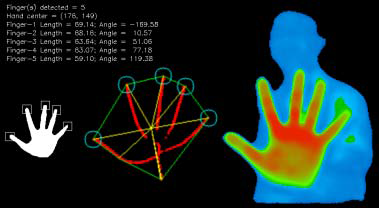
\includegraphics[width=0.75\textwidth]{FingerDetectionUsingDepthData}
\caption{Finger Detection using Depth Data \cite{NIRGesture14}}
\label{FingerDetectionUsingDepthData}
\end{figure}%
%
\cite{NIRGesture14} proposed another smart and real-time depth camera based on a new depth generation principle. A monotonic increasing and decreasing function is used to control the frequency and duty-cycle of the NIR illumination pulses. The adjusted light pulses reflect off of the object of interest and are captured as a series of images. A reconfigurable hardware architecture calculates the depth-map of the visible face of the object in real-time from a number of images. The final depth map is then used for gesture detection, tracking and recognition. Fig.~\ref{FingerDetectionUsingDepthData} shows an example extraction of hand skeleton. In 2013, Jaehong \cite{InteractiveManipulation_2013} \textit{et al}. develop and implement a Kinect-based 3D gesture recognition system for interactive
manipulation of 3D objects in educational visualization softwares. 
\\\indent%
%%%
%%%
%%%
%%% SLAM --> accuracy
%%%
%%% indoor perception, SLAM, 
\\\indent
RGB-D cameras own great credits in mobile robotics building dense 3D maps of indoor environments. Such maps have applications in robot navigation, manipulation, semantic mapping, and telepresence. \cite{indorMappingRGBD_2014} present a detailed RGB-D mapping system that utilizes a joint optimization algorithm combining visual features and shape-based alignment. Building on best practices in Simultaneous Localization And Mapping (SLAM) and computer graphics makes it possible to build and visualize accurate and extremely rich 3D maps with RGB-D cameras. Visual and depth information are also combined for view-based loop closure detection, followed by pose optimization to achieve globally consistent maps. SLAM is the process of generating a model of the environment around a robot or sensor, while simultaneously estimating the location of the robot or sensor relative to the environment. SLAM has been performed in many ways, which can be categorized generally by their focus on localization or environment mapping \cite{SLAMintro_2015}. SLAM systems focused on localizing the sensor accurately, relative to the immediate environment, make use of sparse sensor data to locate the sensor. Using range sensors such as scanning laser range-finders \cite{laserSLAM_2011}, LiDAR and SONAR \cite{sonarSLAM_2013}, many robot applications use SLAM systems only to compute the distance from the sensor to the environment. SLAM systems focused on mapping use dense sensor output to create a high-fidelity 3D map of the environment, while using those data to also compute relative location of the sensor \cite{KinectFusion_2011} \cite{mapSLAM_2013}. Many modern SLAM algorithms combine both approaches, usually by extracting sparse features from the sensor and using these for efficiently computing the location of the sensor. This position is then used to construct a map from dense sensor data. 
\\\indent
With a consumer RGB-D camera providing both color images and dense depth maps at full video frame rate, there appears a novel approach to SLAM that combines the scale information of 3D depth sensing with the strengths of visual features to create dense 3D environment representations, which is called RGB-D SLAM. \cite{RGBDSLAM01_2012} gives an open source approach to visual SLAM from RGB-D sensors, which extracts visual keypoints from the color images and uses the depth images to localize them in 3D. %
%
\begin{figure}[t]
\centering
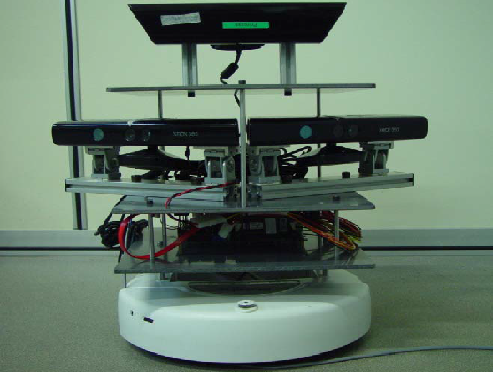
\includegraphics[width=0.5\textwidth]{threeKinect}
\caption{SLAM system with Only RGBD Cameras \cite{RGBDSLAMsystem_2013}}
\label{threeKinect}
\end{figure}%
%
\cite{RGBDSLAMsystem_2013} builds an efficient SLAM system using three RGBD sensors. As shown in fig.~\ref{threeKinect}, one Kinect looking up toward the ceiling can track the robot’s trajectory through visual odometry method, which provide more accurate motion estimation compared to wheel motion measurement without being disturbed under wheel slippage. And the other two contiguous horizontal Kinects can provide wide range scans, which ensure more robust scan matching in the RBPF-SLAM framework. Also using RGB-D sensor for SLAM, \cite{bundleSLAMRGBD_2015} presents a constraint bundle adjustment which allows to easily combine depth and visual data in cost function entirely expressed in pixel. In order to enhance the instantaneity of SLAM for indoor mobile robot, \cite{indorRGBDSLAM_2015} proposed a RGBD SLAM method based on Kinect camera, which combined Oriented FAST and Rotated BRIEF (ORB) algorithm with Progressive Sample Consensus (PROSAC) algorithm to execute feature extracting and matching. %
%
%
\begin{figure}[t]
\centering
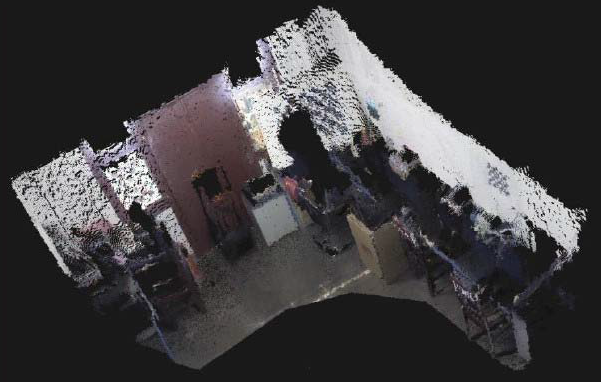
\includegraphics[width=0.7\textwidth]{3DpointCloudMapOfLab}
\caption{3D Map of RGBD-SLAM with ORB and PROSAC \cite{indorRGBDSLAM_2015}}
\label{3DpointCloudMapOfLab}
\end{figure}%
%
ORB algorithm which has better property than many other feature descriptors was used for extracting feature. At the same time, ICP algorithm was adopted for coarse registration of the point clouds, and PROSAC algorithm which is superior than RANSAC in outlier removal was employed to eliminate incorrect matching. To make the result more accurate, pose-graph optimization was achieved based on General Graph Optimization (g2o) framework. Fig.~\ref{3DpointCloudMapOfLab} shows the 3D volumetric map of the lab, which can be directly used to navigate robots.
\\\indent%
%%
%A robot, for example, needs to know its location in the world to navigate between places. This problem is a classical and challenging chicken-and-egg problem because localizing the camera in the world requires the 3D model of the world, and building the 3D model in turn requires the pose of the camera. Therefore, both the camera trajectory and the 3D model need to be estimated at the same time.
RGB-D camera is also famous in application of doing visual odometry on autonomous flight of a micro air vehicle (MAV), helping acquire 3D models of the environment and estimate the camera pose with respect to the environment model. Visual odometry generally has unbounded global drift while estimating local motion. To bound estimation error, it can be integrated with SLAM algorithms, which employ loop closing techniques to detect when a vehicle revisits a previous location. A computationally inexpensive RGBD-SLAM solution is discussed by \cite{RGBDSLAMmav_2013} tailored to the application on autonomous MAVs, which enables our MAV to fly in an unknown environment and create a map of its surroundings completely autonomously, with all computations running on its onboard computer. Fig.~\ref{RGBD_SLAM_MAV} shows the MAC with an RGB-D sensor (the first generation of Kinect) mounted. And fig.~\ref{mavReconstruction} shows the reconstruction based on the full point clouds, with the estimated trajectory shown in red dots. 
%
\\\indent
%
\begin{figure}[t]
\centering
\subfloat[RGBD UAV]{
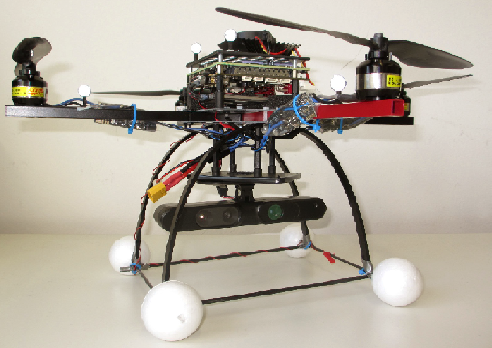
\includegraphics[height=0.4\textwidth , width = 0.5\textwidth]{RGBD_SLAM_MAV}
\label{RGBD_SLAM_MAV}}
\subfloat[Reconstruction and Estimated Trajectory]{
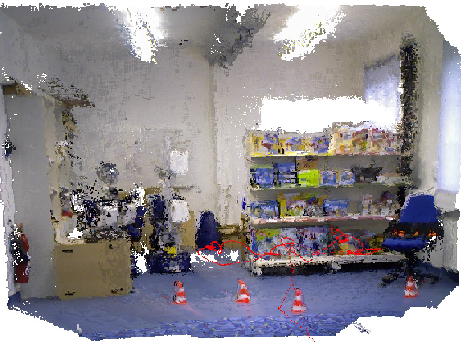
\includegraphics[height=0.4\textwidth , width = 0.5\textwidth]{mavReconstruction}
\label{mavReconstruction}}
%\qquad
\caption{RGBD-SLAM for Autonomous MAVs \cite{RGBDSLAMmav_2013}}
\label{autoRGBD_SLAM_MAV}
\end{figure}%
% Volumetric Reconstruction and Virtual Reality : 3D printing, Kinect fusion
% KinectFusion, 3D printing
RGB-D sensors can be used on a much smaller scale than SLAM to create more detailed, volumetric reconstructions of objects and smaller environments, which opens a new world to the fast 3D printing. 3D printing is an additive technology in which 3D objects are created using layering techniques of different materials, such as plastic, metal, \textit{etc}.  It has been around for decades, but only recently is available and famous among the general public. The first 3D printing technology developed in the 1980’s was stereolithography (SLA) \cite{Patent3Dprinting86}. This technique uses an ultraviolet (UV) curable polymer resin and an UV laser to build each layer one by one. Since then other 3D printing technologies have been introduced. Nowadays, some companies like iMaterialise or Shapeways offer 3D printing services where you can simply upload your CAD model on-line, choose a material and in a few weeks your 3D printed object will be delivered to your address. This procedure is quite straight-forward when you got your CAD model. However, 3D shape design tends to be a long and tedious process, with the design of a detailed 3D part usually requiring multiple revisions. Fabricating physical prototypes using low cost 3D fabrication technologies at intermediate stages of the design process is now a common practice, which helps the designer discover errors, and to incrementally refine the design. Most often, implementing the required changes directly in the computer model, within the 3D modeling software, is more difficult and time consuming than modifying the physical model directly using hand cutting, caving and sculpting tools, power tools, or machine tools. When one of the two models is modified, the changes need to be transferred to the other model, a process we refer to as synchronization. 
\\\indent
KinectFusion, a framework that allows a user to create a detailed 3D reconstruction of an object or a small environment in real-time using Microsoft Kinect sensor, has garnered a lot of attention in the reconstruction and modeling field. It enables a user holding and moving a standard Kinect camera to rapidly create detailed 3D reconstructions of an indoor scene \cite{KinectFusionIzadi_2011}. Not only an entire scene, a specific smaller physical object could also be cleanly segmented from the background model simply by moving the object directly. Fig.~\ref{FastDirectObjectSegmentation} shows how the interested object (a teapot) is accurately segmented from the background by physically removed. The sub-figure (A) shows surface normals, and sub-figure (B) is the texture mapped model. %
%
\begin{figure}[t]
\centering
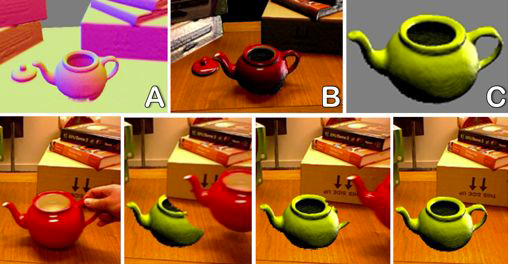
\includegraphics[width=0.7\textwidth]{FastDirectObjectSegmentation}
\caption{Object Segmentation in KinectFusion \cite{KinectFusionIzadi_2011}}
\label{FastDirectObjectSegmentation}
\end{figure}%
%
\cite{3DPrintingFrom3DSensing13} proposed and introduced a from-Sense-to-Print system that can automatically generate ready-to-print 3D CAD models of objects or humans from 3D reconstructions using the low-cost Kinect sensor. Further, \cite{3DModelingForPrinting15} addresses the problem of synchronizing the computer model to changes made in the physical model by 3D scanning the modified physical model, automatically detecting the changes, and updating the computer model. A new method is proposed that allows the designer to move fluidly from the physical model (for example his 3D printed object, or his carved object) to the computer model. In the proposed process the physical modification applied by the designer to the physical model are detected by 3D scanning the physical model and comparing the scan to the computer model. Then the changes are reflected in the computer model. The designer can apply further changes either to the computer model or to the physical model. Changes made to the computer model can be synchronized to the physical model by 3D printing a new physical model.
%
%
%%%%%%%%%%%%%%%%%%%%%%%%%%%%%%%%%%%%%%%%%%%%%%%%%%%%%%%
%%%%%%%%%%                                                     %%%%%%%%%%%%%%%%%%%%%%%%%%%
%%%%%%%%%%  1.3   Calibration of RGB-D Cameras         %%%%%%%%%%%%%%%%%%%%%%%%
%%%%%%%%%%                                                     %%%%%%%%%%%%%%%%%%%%%%%%
%%%%%%%%%%%%%%%%%%%%%%%%%%%%%%%%%%%%%%%%%%%%%%%%%%%%%%%
\section{Calibration of RGB-D Cameras}
\label{sectionRGBDcameraCalibration}
\indent
Camera calibration is a necessary step in 3D computer vision in order to extract metric information from 2D images. The calibration of a RGB-D camera aims to be able to generate the world coordinates (\(X^W, Y^W, Z^W\)) with corresponding \(RGB\) values for every single pixel, given the depth steams and RGB streams retrieved from the camera. During the camera calibration, the removal of lens distortions must be involved in order to get the undistorted 3D reconstruction, especially for consumer cameras that utilize a low-cost lens. Imperfect lens shape causes light rays bending more near the edges of a lens than they do at its optical center. The smaller the lens, the greater the distortion. With a wide-angle lens where the field of view of the lens is much wider than the size of the image sensor, barrel distortions will commonly happen. For example, fig.~\ref{NIR_by_Depth_front} shows KinectV2's raw (without distortion removal) NearIR 3D image observing a flat wall, on which a canvas printed with uniform grid dots pattern is hung. A blue rectangle is dropped onto the image, which helps show the \enquote{barrel-shape} deformation of the uniform grid pattern.
\\\indent
For decades, much work on camera calibration has been done, starting from the photogrammetry community \cite{photogrammetry01_1971} \cite{photogrammetry02_1975}, to computer vision (\cite{Tsai1987} \cite{treeDcalibration1_1993} \cite{Zhengyou04} to cite a few). After the release of the low-cost Microsoft Kinect, a lot of researchers focus their calibrations specially on RGB-D cameras (\textit{e.g.}, Kinect). Jan \textit{et al}. \cite{KinectCali01_2011} analyze Kinect as a 3D measuring device, experimentally investigate depth measurement resolution and error properties and make a quantitative comparison of Kinect accuracy with stereo reconstruction from SLR cameras and a 3D-TOF camera. Using small data sets of Kinect, Carolina \textit{et al}. \cite{KinectCali02_2013} present a new method for calibrating a color-depth camera pair, which prevents the calibration from suffering a drift in scale. Aaron \textit{et al}. \cite{KinectCali03_2015} presented a novel multi-Kinect calibration algorithm that only requires a user to move single spherical object in front of the Kinects observed from multiple viewpoints.
\\\indent
%
 \begin{figure}[b]
%\centering
\subfloat[Front View][Front View]{

\includegraphics[height=0.42\textwidth]{NIR_by_Depth_front}
\label{NIR_by_Depth_front}}
\subfloat[Left View][Left View]{

\includegraphics[height=0.42\textwidth , width = 0.4\textwidth]{NIR_by_Depth_LeftSide}
\label{NIR_by_Depth_LeftSide}}
%\qquad
\caption{Raw Distorted KinectV2 NearIR 3D Reconstruction}
\label{NearIR}
\end{figure}%
%
However, those camera calibration methods, using limited number of points to train the non-linear distortion-removal model, are not able to cover all pixels of a sensor. Besides, with one pinhole camera model (3-by-4 transformation matrix) for raw (deformed) 3D reconstruction and another model to remove lens distortion, the final 3D reconstruction cannot be displayed efficiently in real-time. What's worse, those calibration methods are assuming that the depth sensor offers perfectly same precision depth value for all pixels. Whereas in practical depth sensors always have some defects in getting same depth accuracy for all of their pixels, which we will call as \enquote{Depth Distortion}. Kourosh and Sander \cite{KinectAccuracy_2012} provide an analysis of the accuracy and resolution of Kinect's depth data. They show that the random error of depth measurement increases with increasing distance to the sensor, and ranges from a few millimeters up to about 4 cm at the maximum range of the sensor. Fig.~\ref{NIR_by_Depth_LeftSide} shows the side view of KinectV2's raw 3D NearIR image observing the wall, and the blue straight line is added on the left side of the 3D reconstruction. We can tell that most pixels on the left side border are apparently not sitting on a straight line.%
\\\indent
%
\begin{figure}[t]
\centering
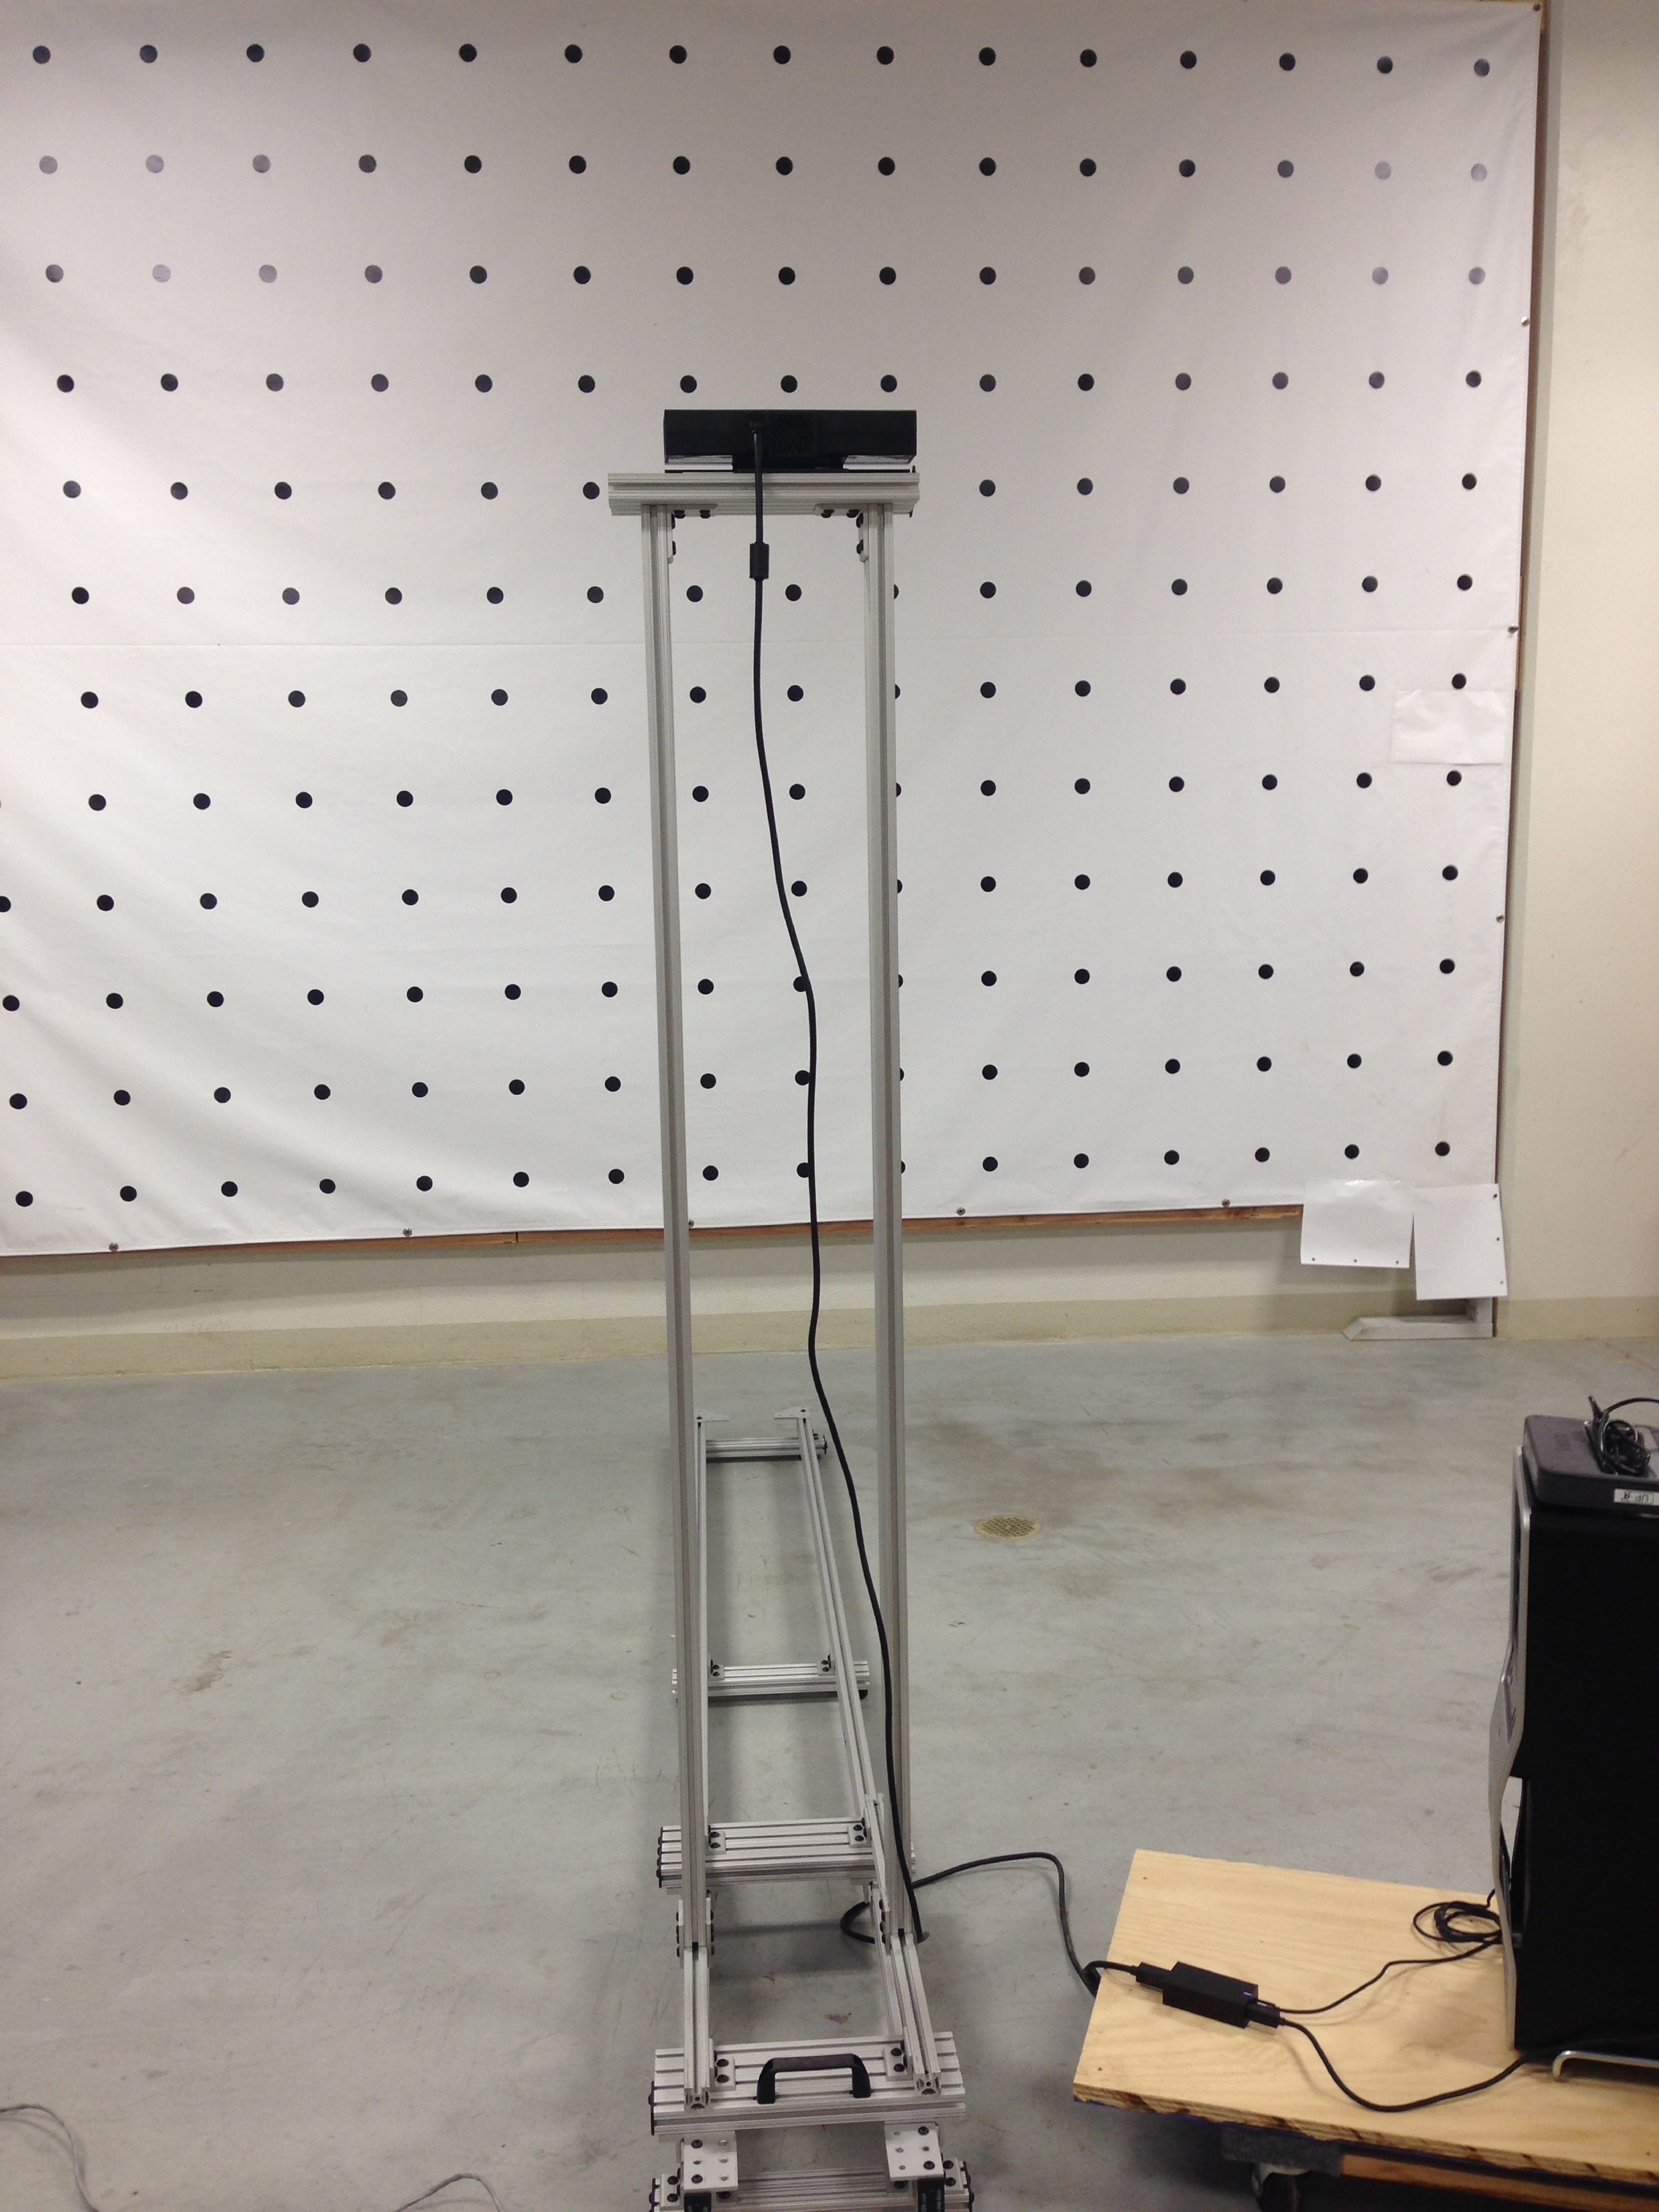
\includegraphics[width=0.55\textwidth]{trackingModuleOnKinectV2CalibrationSystem}
\caption{KinectV2 Calibration System}
\label{trackingModuleOnKinectV2CalibrationSystem}
\end{figure}%
%
In order to get enough calibrating points that can cover all pixels of the sensor, as well as solving the \enquote{Depth Distortion}, a moving plane with camera on rail calibration system is introduced in this thesis. As shown in figure \ref{trackingModuleOnKinectV2CalibrationSystem}, the rail is perpendicular to the uniform round dots pattern, along with the \(Z^{w}\) axis. A RGB-D camera KinectV2 is mounted on the top of the slider, whose moving along the rail generates same effect as a moving pattern plane. This calibration system makes it possible to do per-pixel \enquote{Depth Distortion} calibration.%
%
%
%%%%%%%%%%%%%%%%%%%%%%%%%%%%%%%%%%%%%%%%%%%%%%%%%%%%%%%
%%%%%%%%%%                                                     %%%%%%%%%%%%%%%%%%%%%%%%%%%
%%%%%%%%%%  1.4     Summation                         %%%%%%%%%%%%%%%%%%%%%%%%
%%%%%%%%%%                                                     %%%%%%%%%%%%%%%%%%%%%%%%
%%%%%%%%%%%%%%%%%%%%%%%%%%%%%%%%%%%%%%%%%%%%%%%%%%%%%%%
\section{Summation}
\indent
A RGB-D camera is a sensing system that capture RGB images along with per-pixel depth information. It opens a new epoch for three-dimensional (3D) markets. RGB-D cameras have both of lens distortions and depth distortion problems. Distortions correction is wildly discussed in image processing area, however, the traditional camera calibration methods are not ideal on accuracy and efficiency. They separated the lens distortion removal from the 3D reconstruction (based on pinhole camera model), which depresses the efficiency of image processing. Moreover, they neither cover all pixels of a sensor when training the distortion model, nor include the depth distortion correction (assuming that the depth values have exact same resolution among every single pixel).%
\\\indent
In this thesis, a novel per-pixel calibration method with look-up table based 3D reconstruction in real-time is introduced, using a rail calibration system shown in fig.~\ref{trackingModuleOnKinectV2CalibrationSystem}. Instead of using a pinhole camera model, which in practical is not ideally accurate, our new proposed calibration method is based on real data. Not only \(X^w\)/\(Y^w\) values are calibrated directly through one step transformation, but \(Z^w\) is also guaranteed accurate by importing externally measured data. Both of the lens distortions and \enquote{depth distortion} could be solved with the help of the rail system.
\\\indent
In Chapter 2, a pinhole-camera-model based calibration method is discussed in detail, including the lens distortions removal as the second step. The proposed data-based calibration method is well explained in Chapter 3, where two polynomial models will be introduced. One lens-distortions removal model helps map directly from image plane \(row\) and \(column\) to \(X^{w}\) and \(Y^{w}\) separately, during calibration data collection. And another \enquote{depth distortion} removal model helps map per-pixel depth (\(D\)) to \(Z^W\) when generating look-up table for per-pixel beam equation. \(Z^{w}\) values will be totally supported from external (a laser distance measurer). The calibration results and real-time 3D reconstruction will be discussed in Chapter 4. Finally, a \(row\) by \(column\) by 6, three dimensional look-up table will be generated for real-time 3D reconstruction. Chapter 5 will talk the future work of RGB-D cameras calibration.
%
%
%
%
%
%
%





%Noises among depth data vary randomly, camera by camera and pixel by pixel; which means a rough point-cloud plane full of bumps and hollows will be reconstructed even though the camera is observing a wall. 




%
%\begin{table}[ht]
%\begin{center}
%\caption{ 3D profile acquisition Taxonomy}
%\label{3DImagingTaxonomy}
%\hspace*{-1cm}
%\begin{tabular}{ |>{\small}l|>{\small}l|>{\small}l|>{\small}l| }
%\hline
%\multicolumn{4}{|c|}{3D Shape Extraction} \\
%\hline
%\multicolumn{2}{|c|}{Passive}  & \multicolumn{2}{c|}{Active}\\
%\hline
%Single Vantage Point & Multiple Vantage Points & Single Vantage Point & Multiple Vantage Points\\
%\hline
%\multirow{5}{*}{
%\makecell[l]{
%\textbullet \, Shape from Texture\\ 
%\textbullet \, Shape from Occlusion\\
%\textbullet \, Time to Contact\\
%\textbullet \, Shape from Defocus\\
%\textbullet \, Shape from Contour}
%} 
%&
%\multirow{5}{*}{\makecell[l]{
%\textbullet \, Passive Stereo\\ 
%\textbullet \, Structure from Motion\\
%\textbullet \, Shape from Silhouettes}
%}
%&
%\multirow{5}{*}{\makecell[l]{
%\textbullet \, Time of Flight\\ 
%\textbullet \, Shape from Shading}
%} 
%&
%\multirow{5}{*}{\makecell[l]{
%\textbullet \, Structured Light\\ 
%\textbullet \, Active Stereo\\
%\textbullet \, Photometric Stereo}
%} \\ & & &
%\\ & & &	\\ & & &	\\ & & &\\
%\hline
%
%\end{tabular}
%\end{center}
%\end{table}





















%\copyrightnotice
%% Chapter 2
\chapter{Traditional \gls{RGBD} Cameras Calibration} % Main chapter title
\label{chapterTraditionalCalibration} % For referencing the chapter elsewhere, use \ref{sens_introduction} 
%\indent
A pinhole-camera model can be used to describe an image sensor's field of view. When applying the pinhole camera model in world space, it explains the mapping relationship from world space to camera space, and then to image space. A $3\times4$ pinhole-camera matrix expresses the mappings mathematically. It consists of an intrinsic matrix mapping from the \gls{3D} camera space to 2D image space, and an extrinsic matrix map from \gls{3D} world space to \gls{3D} camera space. Traditionally, lens distortions correction is after, and separated from the pinhole-camera model calibration. In this chapter, we will introduce the camera calibration methods based on the pinhole-camera model in detail, and then discuss how to remove the lens distortions in traditional methods.
%
\begin{figure}[!b]
\centering
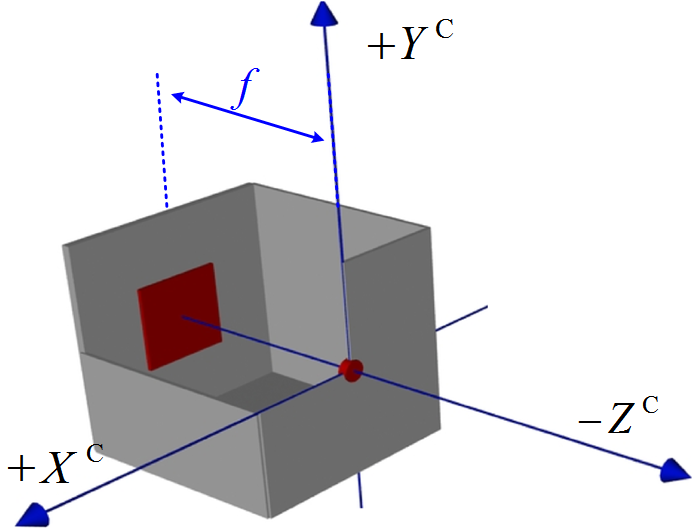
\includegraphics[width=0.45\textwidth]{PinholeCameraFigure}
\caption{The Pinhole Camera Inspection}
\label{PinholeCameraFigure}
\end{figure}%
%%
\section{Pinhole Camera}
\label{sectionPinholeCamera}
%%%%%%%%%%%%%%%%%%%%%%%%%%%%%%%%%%%%%%%%%%%%%%%%%%%%%
%%%%%%%%%%                                                                                                   %%%%%%%%%%
%%%%%%%%%%      1. Intrinsic, introduce camera model from \gls{3D} to 2D:         %%%%%%%%%%%
%%%%%%%%%%                 (X^c, Y^c, Z^c) --> \(r, \, c\)                                          %%%%%%%%%%%
%%%%%%%%%%%%%%%%%%%%%%%%%%%%%%%%%%%%%%%%%%%%%%%%%%%%%%
\indent
A pinhole camera is a simple optical imaging device in the shape of a closed box or chamber. A pinhole camera is completely dark on all the other sides of the box including the side where the pin-hole is created. Figure~\ref{PinholeCameraFigure} shows an inspection of a pinhole camera. In its front is a pin-hole that help create an image of the outside space on the back side of the box. When the shutter is opened, the light shines through the pin-hole and imprint an image onto a sensor (or photographic paper, or film) placed at the back side of the box. In order to analyze parameters like focal distance, field of view, etc., pinhole camera has its own three dimensional space (noted as \(\gls{cameraX}\), \(\gls{cameraY}\), and \(\gls{cameraZ}\)). Note that, according to Cartesian Coordinates \enquote{right hand} principle, the camera is looking down the negative of \(\gls{cameraZ}\)-axis, given \(\gls{cameraX}\)\(\gls{cameraY}\) directions as shown in the figure. Its focal length of the pinhole camera is the distance on the \(Z^c\)-axis, between the pinhole at the front of the camera and the paper or film at the back of the camera.
\\\indent
\begin{figure}[!t]
\centering
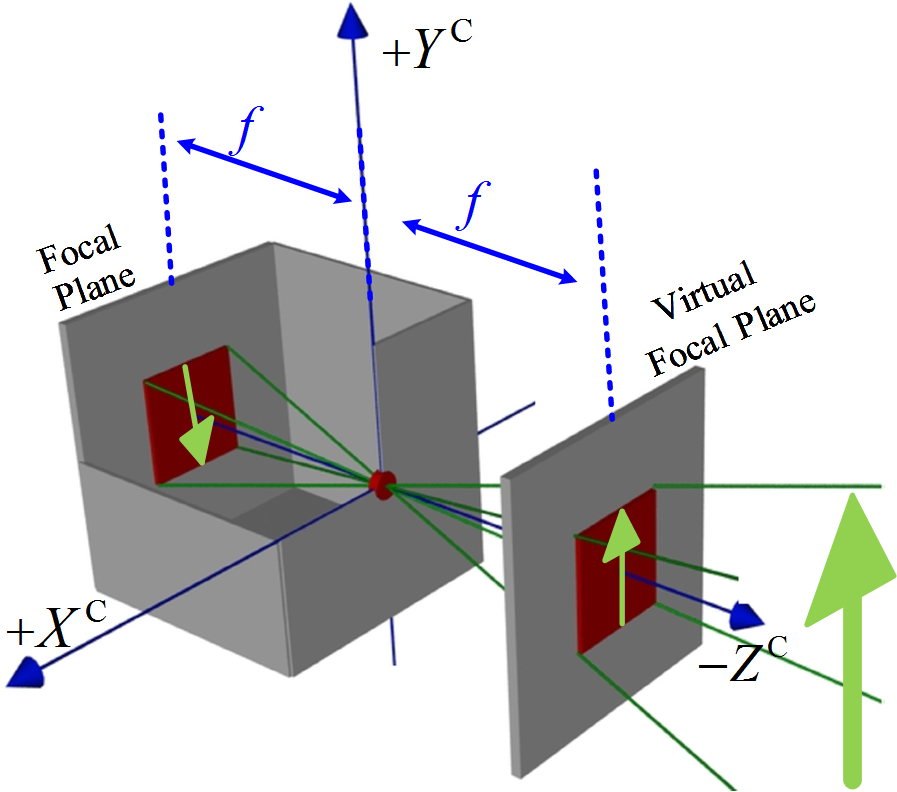
\includegraphics[width=0.5\textwidth]{PinHoleVirtualFocalPlane}
\caption{Virtual Focal Plane of a Pinhole Camera}
\label{PinHoleVirtualFocalPlane}
\end{figure}%
%
%
Pinhole cameras are characterized by the fact that they do not have a lens. It rely on the fact that light travels in straight lines, which is a principle called the rectilinear theory of light. This makes the image appear upside down in the camera, as shown in Fig.~\ref{PinHoleVirtualFocalPlane}. Tracing the corners of the camera sensor through the pin hole, those dark green lines show the limits of the field of view in \gls{3D} coordinate space. The back side plane of the pinhole camera, which is behind the origin at a positive \(\gls{cameraZ}\)-axis and also where our sensor sits, is also called the focal plane. It is not intuitive, nor convenient for mathematical analysis that the images on the focal plane are always upside down. So a virtual focal plane is defined in front of the pinhole on the negative \(\gls{cameraZ}\)-axis, which is equal distant from the focal point (pin hole) as the actual focal plane is behind. Notice that the limits of the field of view intersect with the virtual focal plane at the four corners of the up-right image just as they disseminate from the four corners of the sensor at the real focal plane.

\begin{figure}[t]
\centering
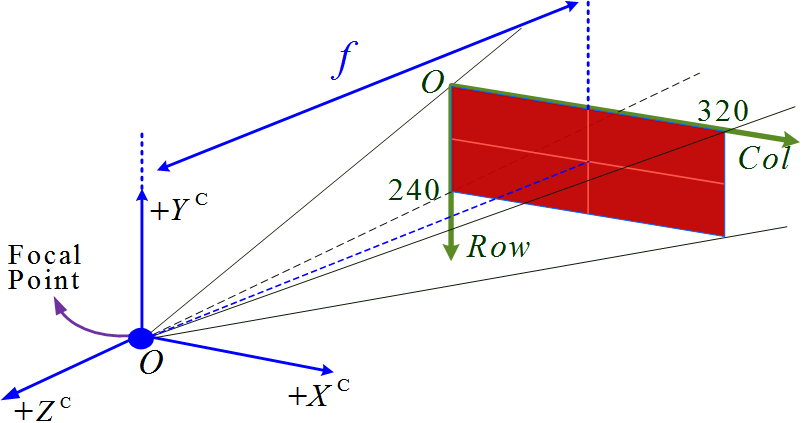
\includegraphics[width=0.65\textwidth]{CommonPinholeCameraModel}
\caption{Common Pinhole Camera Model for a $240\times320$ Pixels Camera Sensor}
\label{CommonPinholeCameraModel}
\end{figure}%
%

With the virtual focal plane, the camera body with the real focal plane could be removed. And the rest parts in front of the the camera body, the focal point and the virtual focal plane together, form the most common pinhole camera model. In order to employ this model to analyze arbitrary \gls{3D} object points inside the camera's field of view in 2D image space, the prior step is to define the relationship between points in \gls{3D} camera space and the 2D image space (\(\gls{imageRow}\) and \(\gls{imageColumn}\)). As shown in Fig.~\ref{CommonPinholeCameraModel}, The focal point is right at the origin of the camera \gls{3D} space coordinates, from where to the sensor is the vertical distance of \(f\), the focal distance. The 2D image coordinates are in dark green, and its origin is sitting at the up-left corner of the sensor. Only the a virtual sensor (in color red) is visible on the virtual focal plane, whose size in 2D image space is noted as 240 by 320 (using the size of PrimeSense camera). As long as both of the camera \gls{3D} space coordinates and image 2D space coordinates are defined, the next job is to build a mapping between them.
%
\begin{figure}[t]
\centering
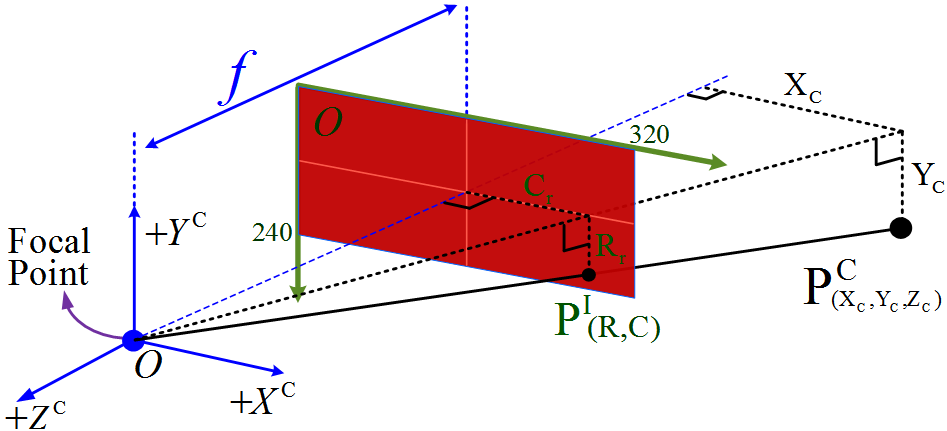
\includegraphics[width=0.82\textwidth]{RelationshipCameraToImage}
\caption{Mapping from Camera Space to Image Space}
\label{RelationshipCameraToImage}
\end{figure}%
%

Select a random object point \(P^C\) in the camera space located at camera \gls{3D} coordinates (\(\gls{cameraPointX0}\), \(\gls{cameraPointY0}\), \(\gls{cameraPointZ0}\)). A line passing both of the point \(P^C\) and the \emph{Focal Point} intersects with the virtual focal plane at \(P^I\), with its image 2D coordinates (\(r, \, c\)). To determine the mapping function, we can start a the proportional relationship. As shown in Fig.~\ref{RelationshipCameraToImage}, the center point in the image coordinates, which is usually called \emph{\gls{principlePoint}}, could be determined by column of half-width (\(c_h\)) and row of half-height (\(r_h\)). Concretely, the \gls{principlePoint} (\(r_h\), \(c_h\)) is either (119.5, 159.5) if range is ([0:239], [0:319]), or (120, 320) if range is ([1:240], [1:320]). So, we could get the relative row and column distance of  \(r_r\) and \(c_r\) by:
%
\begin{equation}
\begin{aligned}
r_r &= r - r_h%
\\%
c_r &= c - c_h \ \ \ .%
\end{aligned}
\label{relativeCRforProportional}
\end{equation}%
%
Based on by triangulation, it is straight forward to tell the proportional relationship between \(f\)/\(\gls{cameraPointZ0}\) and \(c_r\)/\(\gls{cameraPointX0}\), \(r_r\)/\(\gls{cameraPointY0}\). Thus we get
%
\begin{equation}
\left[ \begin{array}{c} c_r \\ r_r \end{array} \right] %
= f %
\left[ \begin{array}{c} \gls{cameraPointX0}/\gls{cameraPointZ0} \\ \gls{cameraPointY0}/\gls{cameraPointZ0} \end{array} \right]  .%
\label{twoDRelativeFromCamToIm}
\end{equation}
\noindent
And by changing the relative distance \(r_r / c_r\) back to the 2D image coordinates \(r, \, c\), then eqn.~(\ref{twoDRelativeFromCamToIm}) will be written as
%
\begin{equation}
\left[ \begin{array}{c} c \\ r \end{array} \right] %
= f %
\left[ \begin{array}{c} \gls{cameraPointX0}/\gls{cameraPointZ0} \\ \gls{cameraPointY0}/\gls{cameraPointZ0} \end{array} \right]%
+
\left[ \begin{array}{c}  c_h \\  r_h \end{array} \right] .%
\label{linearRelationFromCamToIm}
\end{equation}
\noindent
If written in homogeneous coordinates, we will get eqn.~(\ref{HomoProportionalRelationFromCamToIm}):
\begin{equation}
%
\gls{cameraPointZ0} \left[ \begin{array}{c} c \\ r \\ 1 \end{array} \right] %
= %
\left[ \begin{array}{c} fx^c \\ fy^c \\ \gls{cameraPointZ0} \end{array} \right]%
+
\left[ \begin{array}{c}  \gls{cameraPointZ0}c_h \\  \gls{cameraPointZ0}r_h \\ 0\end{array} \right] %
=  \begin{bmatrix} f & 0 &  c_h  \\ 0 & f & r_h \\ 0 & 0 & 1 \end{bmatrix}%
\left[ \begin{array}{c} \gls{cameraPointX0} \\ \gls{cameraPointY0} \\ \gls{cameraPointZ0} \end{array} \right] .%
\label{HomoProportionalRelationFromCamToIm}
\end{equation}%
%
\\\indent
Till Now, we haven't consider the units translation between the camera \gls{3D} space the image 2D space. The random object point \(P^C\)'s mapping point \(P^I\) (\(r, \, c\)) on the image space is expressed in millimeters (or inches). Since it is necessary to express the image space coordinates (\(r, \, c\)) in pixels, we need to find out the resolution of the sensor in pixels/millimeter. Considering that, the pixels are not necessarily be square-shaped, we assume they are rectangle-shaped with resolution  $\alpha_c$ and \(\alpha_r\) pixels/millimeter in the \(\gls{imageColumn}\) and \(\gls{imageRow}\) direction respectively. Therefore, to express \(P^I\) in pixels, its \(c\) and \(r\) coordinates should be multiplied by \(\alpha_c\) and \(\alpha_r\) respectively, to get:
%
\begin{equation}
\left[ \begin{array}{c} \gls{cameraPointZ0} c \\ \gls{cameraPointZ0} r \\ \gls{cameraPointZ0}  \end{array} \right] %
= %
\left[ \begin{array}{c} f\alpha_c x^c \\ f \alpha_r y^c \\ \gls{cameraPointZ0} \end{array} \right]%
+
\left[ \begin{array}{c}  \gls{cameraPointZ0} \alpha_c c_h \\ \gls{cameraPointZ0} \alpha_r r_h \\ 0 \end{array} \right] %
=  \begin{bmatrix} \alpha_c f & 0 &  \alpha_c c_h  \\ 0 & \alpha_r f & \alpha_r r_h \\ 0 & 0 & 1 \end{bmatrix}%
\left[ \begin{array}{c} \gls{cameraPointX0} \\ \gls{cameraPointY0} \\ \gls{cameraPointZ0} \end{array} \right]%
= \gls{intrinsicMatrixK} \textbf{\textit{P}}^C  .
\label{HomoProportionalFromCamToImInPixels}
\end{equation}%

\noindent
Note that \(\gls{intrinsicMatrixK}\) only depends on the intrinsic camera parameters like its focal length, resolution in pixels, and sensor's width and height. Thus, the mapping matrix \(\gls{intrinsicMatrixK}\) is also called a camera's intrinsic matrix. Considering that the pixels might be parallelogram-shaped instead of rigid rectangle-shaped (when the image coordinate axis \(\gls{imageRow}\) and \(\gls{imageColumn}\) are not orthogonal to each other), usually \(\gls{intrinsicMatrixK}\) has a skew parameter \(s\), given by

\begin{equation}
\gls{intrinsicMatrixK}%
=  \begin{bmatrix} 
f_c & s & t_c \\
 0 & f_r & t_r \\
 0 & 0 & 1 \end{bmatrix} ,%
\label{intrinsicKmatrix}
\end{equation}%
\noindent
where \(f_c = \alpha_c f\) and \(f_r = \alpha_r f\) are the focal length in pixels on the \(\gls{imageColumn}\) and \(\gls{imageRow}\) directions respectively,  \(t_c = \alpha_c r_h\) and \(t_r = \alpha_r r_h\) are the translation parameters that help move the origin of image coordinate to the \gls{principlePoint}.
\\\indent
%%%%%%%%%%%%%%%%%%%%%%%%%%%%%%%%%%%%%%%%%%%%%%%%%%%%%
%%%%%%%%%%                                                                                                   %%%%%%%%%%
%%%%%%%%%%      2. Extrinsic, (X^w, Y^w, Z^w) --> (X^c, Y^c, Z^c)          %%%%%%%%%%%
%%%%%%%%%%                                                                                                    %%%%%%%%%%%
%%%%%%%%%%%%%%%%%%%%%%%%%%%%%%%%%%%%%%%%%%%%%%%%%%%%%%
Now we have \(\gls{intrinsicMatrixK}\), which helps map between camera \gls{3D} space and image 2D space. But we are still not able to employ it yet. The camera \gls{3D} space is with respect to the camera sensor only. Neither can we directly tell the camera \gls{3D} coordinates of an object point, nor can we assign it. All we can do is to use the camera space as an intermediate space between the image coordinates and world coordinates, which we could assign by ourselves. %
%
\begin{figure}[!t]
\centering
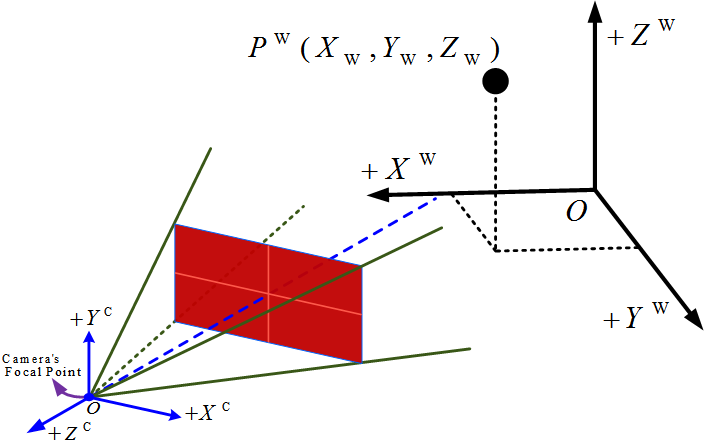
\includegraphics[width=0.65\textwidth]{FromWorldToCameraSpace}
\caption{Pinhole Camera in World Space}
\label{FromWorldToCameraSpace}
\end{figure}%
%
Figure~\ref{FromWorldToCameraSpace} shows a pinhole camera observing an arbitrary object point P in the world  space. We assign the world coordinates so that the object point has world space coordinates \(P^W(x^w, \, y^w, \, z^w)\). Although the world space and camera space are two different spaces, we could easily transform between each other through rotation and translation, as long as both of the spaces are using rigid Cartesian Coordinates. With a standard rotation matrix \(\gls{exRotationR}\) and a translation matrix \(\gls{exTranslationT}\)
%
\begin{equation}
\gls{exRotationR}%
=  \begin{bmatrix} 
r_{11} & r_{12} & r_{13} \\
r_{21} & r_{22} & r_{23} \\
r_{31} & r_{32} & r_{33}
 \end{bmatrix}%
, \, \, 
\gls{exTranslationT}%
=  \begin{bmatrix} 
t_{1} \\
t_{2} \\
t_{3}
 \end{bmatrix} ,%
\label{rotationTranslationMatrixRT}
\end{equation}%
%
we can get the transformation matrix \([\gls{exRotationR} \,\, \gls{exTranslationT}]\) from the world space to camera space:
%
\begin{equation}
\begin{bmatrix} 
X^{C} \\
Y^{C} \\
Z^{C}
 \end{bmatrix}%
=  \gls{exRotationR} \begin{bmatrix} 
X^{W} \\
Y^{W} \\
Z^{W}
 \end{bmatrix}%
 + \gls{exTranslationT}
=
\begin{bmatrix} 
\gls{exRotationR} & \gls{exTranslationT} \\
\end{bmatrix}%
 \begin{bmatrix} 
X^{W} \\
Y^{W} \\
Z^{W} \\
1
 \end{bmatrix}  .%
\label{mappingFromWorldToCameraSpace}
\end{equation}%
%
%%%% 2.5 Pinhole Camera Matrix (X^w, Y^w, Z^w) --> (X^c, Y^c, Z^c) --> \(r, \, c\)
%
\noindent
The parameters that help map from world space to camera space depend on how we assign the world coordinates. Since none of them are from the camera even though they are belongs to an important part of camera calibration, usually the matrix \([\gls{exRotationR} \,\, \gls{exTranslationT}]\) is called extrinsic camera matrix. With both of the extrinsic camera matrix (help map from world space to camera space) and the intrinsic camera matrix (help map from camera space to image space), we are now able to build the connection between the world space coordinates, which could be assigned by ourselves, and the image space \(\gls{imageRow}\) and \(\gls{imageColumn}\), which are the streams we retrieved from the camera. 
\\\indent
To combine the intrinsic camera matrix and extrinsic camera matrix (combine eqn.~(\ref{HomoProportionalFromCamToImInPixels}) and eqn.(~\ref{mappingFromWorldToCameraSpace})), we get 

\begin{equation}
\gls{cameraZ}\left[ \begin{array}{c} C \\ R \\ 1 \end{array} \right] %
=\gls{intrinsicMatrixK} \left[ \begin{array}{c} \gls{cameraX} \\ \gls{cameraY} \\ \gls{cameraZ}\end{array} \right]%
=\gls{intrinsicMatrixK} \begin{bmatrix} \gls{exRotationR} & \gls{exTranslationT} \end{bmatrix} \left[ \begin{array}{c} X^W \\ Y^W \\ Z^W \\ 1 \end{array} \right]%
=\gls{pinHoleCameraM} \left[ \begin{array}{c} X^W \\ Y^W \\ Z^W \\ 1 \end{array} \right]%
 , %
\label{pinholeCameraMatrixCalculation}
\end{equation}%
\noindent
where: %
\begin{equation}
\gls{pinHoleCameraM} = \gls{intrinsicMatrixK} \begin{bmatrix} \gls{exRotationR} & \gls{exTranslationT} \end{bmatrix}%
= \begin{bmatrix} 
m_{11} & m_{12} & m_{13} & m_{14} \\
m_{21} & m_{22} & m_{23} & m_{24} \\
m_{31} & m_{32} & m_{33} & m_{34} \\
\end{bmatrix} . %
\label{pinholeMatrix3x4M}
\end{equation}%
%
\noindent
Note that, although \(\gls{cameraZ}\) values can be retrieved from the depth sensor streams, they will be employed during the calculation of \(\gls{pinHoleCameraM}\), because they will be expressed by the third row parameters in matrix \(\gls{pinHoleCameraM}\). \(\gls{cameraZ}\) will only be used in the step of \gls{3D} reconstruction after the pinhole camera matrix M is determined, as will be discussed in details in Section~\ref{section3DcameraCalibration}. Thus, \(\gls{cameraZ}\) in eqn.~(\ref{pinholeCameraMatrixCalculation}) is commonly substituted as an intermediate parameter \(k\). We did not change \(\gls{cameraZ}\) for the consistency of derivations.
To inspect the pinhole camera matrix \(\gls{pinHoleCameraM}\), it is composed of rotation/translation matrix for \gls{3D} space transforming and intrinsic perspective matrix for handling both of perspective view mapping and shape-skewing, all of which belong to linear processing. In other words, this $3\times4$ transformation matrix is specially for handling perspective view, or perspective distortion. The pinhole camera model is based on the homogeneous coordinates, which means its matrix \(\gls{pinHoleCameraM}\) is also limited by linear processing.
%%%%%%%%%%%%%%%%%%%%%%%%%%%%%%%%%%%%%%%%%%%%%%%%%%%%%
%%%%%%%%%%                                                                                                   %%%%%%%%%%
%%%%%%%%%%      3.        \gls{3D} Reconstruction from Depth                               %%%%%%%%%%%
%%%%%%%%%%                                                                                                    %%%%%%%%%%%
%%%%%%%%%%%%%%%%%%%%%%%%%%%%%%%%%%%%%%%%%%%%%%%%%%%%%%
   
\section{\gls{3D} Camera Calibration}
\label{section3DcameraCalibration}
%    3. Pinhole camera matrix solving for matrix M
\indent
The calibration of a \gls{3D} camera aims to be able to generate the world coordinates (\(\gls{worldX}, \gls{worldY}, \gls{worldZ}\)) and corresponding \(RGB\) values for every single pixel, given the depth steams and RGB streams retrieved from the \gls{3D} camera. From Section~\ref{sectionPinholeCamera}, we know that the pinhole camera matrix \(\gls{pinHoleCameraM}\) (eqn.~(\ref{pinholeMatrix3x4M})) could help map from the world space to image space; however not able to directly transform image space data to world space coordinates. In order to determine \(\gls{worldX}/\gls{worldY}/\gls{worldZ}\) (based on eqn.(~\ref{HomoProportionalFromCamToImInPixels}) and eqn.(~\ref{mappingFromWorldToCameraSpace})), both of the intrinsic camera matrix and extrinsic camera matrix are needed, both of which are intermediate parameters and practically can only be determined through matrix \(\gls{pinHoleCameraM}\). Thus, the first job for \gls{3D} camera calibration is to solve the pinhole camera matrix \(\gls{pinHoleCameraM}\).
\\\indent
To solve the pinhole camera matrix, we can use least squares fit with known \gls{3D} points (\(\gls{worldX}\), \(\gls{worldY}\), \(\gls{worldZ}\)) and their corresponding image points (\(R, C\)). With one point, based on eqn.~(\ref{pinholeMatrix3x4M}) and (\ref{pinholeCameraMatrixCalculation}), we can get two equations.
\begin{equation}
\begin{aligned}
m_{11}\gls{worldX} + m_{12}\gls{worldY} + m_{13}\gls{worldZ} + m_{14} - m_{31}X^WC - m_{32}Y^WC - m_{33}Z^WC - m_{34}C = 0%
\\%
m_{21}\gls{worldX} + m_{22}\gls{worldY} + m_{23}\gls{worldZ} + m_{24} - m_{31}X^WR - m_{32}Y^WR - m_{33}Z^WR - m_{34}R = 0
\end{aligned}
\label{onePointEquationCR}
\end{equation}%
\noindent
There are totally 12 unknowns to solve, thus we need at least six points to solve the $3\times4$ pinhole camera matrix \(\gls{pinHoleCameraM}\). Using $n$-points least squares to solve the best fit, we can build a $2n$ equations matrix, given by eqn.~(\ref{nPoints2nEquationCR}).

\begin{equation}
\hspace*{-1cm}
\begin{bmatrix} 
\gls{worldX}_1 & \gls{worldY}_1 & \gls{worldZ}_1 & 1 & 0 & 0 & 0 & 0 & -\gls{worldX}_1C_1 & -\gls{worldY}_1C_1 & -\gls{worldZ}_1C_1 & -C_1\\
0 & 0 & 0 & 0 & \gls{worldX}_1 & \gls{worldY}_1 & \gls{worldZ}_1 & 1 &  -\gls{worldX}_1R_1 & -\gls{worldY}_1R_1 & -\gls{worldZ}_1R_1 & -R_1\\
\gls{worldX}_2 & \gls{worldY}_2 & \gls{worldZ}_2 & 1 & 0 & 0 & 0 & 0 & -\gls{worldX}_2C_2 & -\gls{worldY}_2C_2 & -\gls{worldZ}_2C_2 & -C_2\\
0 & 0 & 0 & 0 & \gls{worldX}_2 & \gls{worldY}_2 & \gls{worldZ}_2 & 1 &  -\gls{worldX}_2R_2 & -\gls{worldY}_2R_2 & -\gls{worldZ}_2R_2 & -R_2\\
 & & & & & & & \vdots & & & & \\
\gls{worldX}_n & \gls{worldY}_n & Z^n_2 & 1 & 0 & 0 & 0 & 0 & -\gls{worldX}_nC_n & -\gls{worldY}_nC_n & -\gls{worldZ}_nC_n & -C_n\\
0 & 0 & 0 & 0 & \gls{worldX}_n & \gls{worldY}_n & \gls{worldZ}_n & 1 & -\gls{worldX}_nR_n & -\gls{worldY}_nR_n & -\gls{worldZ}_nR_n & -R_n
\end{bmatrix}
\begin{bmatrix} 
m_{11} \\ m_{12} \\ m_{13} \\ m_{14} \\
\vdots
\\ m_{33} \\ m_{34} 
\end{bmatrix}
=
\begin{bmatrix} 
0 \\ 0 \\ 0 \\ 0 \\
\vdots \\ 0 \\ 0
\end{bmatrix}
\label{nPoints2nEquationCR}
\end{equation}%

\noindent
Considering that this matrix is build on homogeneous system, there is no unique solution. There can always be a total-zeros solution. %
\\\indent
To make the solution unique, we select \(m_{34} = 1\), so that the homogeneous eqn.~(\ref{nPoints2nEquationCR}) could be changed into an inhomogeneous format like \(\textbf{\textit{A}}X = B\), where the known matrix \(\textbf{\textit{A}}\) is a $2n\times11$ matrix and known matrix \(B\) is a $2n$ vector:

\begin{equation}
\hspace*{-0.1cm}
\begin{bmatrix} 
\gls{worldX}_1 & \gls{worldY}_1 & \gls{worldZ}_1 & 1 & 0 & 0 & 0 & 0 & -\gls{worldX}_1C_1 & -\gls{worldY}_1C_1 & -\gls{worldZ}_1C_1\\
0 & 0 & 0 & 0 & \gls{worldX}_1 & \gls{worldY}_1 & \gls{worldZ}_1 & 1 &  -\gls{worldX}_1R_1 & -\gls{worldY}_1R_1 & -\gls{worldZ}_1R_1\\
\gls{worldX}_2 & \gls{worldY}_2 & \gls{worldZ}_2 & 1 & 0 & 0 & 0 & 0 & -\gls{worldX}_2C_2 & -\gls{worldY}_2C_2 & -\gls{worldZ}_2C_2\\
0 & 0 & 0 & 0 & \gls{worldX}_2 & \gls{worldY}_2 & \gls{worldZ}_2 & 1 &  -\gls{worldX}_2R_2 & -\gls{worldY}_2R_2 & -\gls{worldZ}_2R_2\\
 & & & & & & & \vdots & & &\\
\gls{worldX}_n & \gls{worldY}_n & Z^n_2 & 1 & 0 & 0 & 0 & 0 & -\gls{worldX}_nC_n & -\gls{worldY}_nC_n & -\gls{worldZ}_nC_n\\
0 & 0 & 0 & 0 & \gls{worldX}_n & \gls{worldY}_n & \gls{worldZ}_n & 1 & -\gls{worldX}_nR_n & -\gls{worldY}_nR_n & -\gls{worldZ}_nR_n
\end{bmatrix}
\begin{bmatrix} 
m_{11} \\ m_{12} \\ m_{13} \\ m_{14} \\
\vdots
 \\ m_{32} \\ m_{33}
\end{bmatrix}
=
\begin{bmatrix} 
C_1 \\ R_1 \\ C_2 \\ R_2 \\
\vdots \\ C_n \\ R_n
\end{bmatrix} .
\label{inHomogenousNPoints2nEquationCR}
\end{equation}%
\noindent
Using pseudo inverse, eqn.~(\ref{inHomogenousNPoints2nEquationCR}) can be solved by \(X = (\textbf{\textit{A}}^T\textbf{\textit{A}})^{-1}\textbf{\textit{A}}^TB\), where \(X\) is an 11-elements vector and \(X(1)\)  \texttildelow \, \(X(11)\) correspond to \(m_{11}\) \texttildelow \, \(m_{33}\). And the $3\times4$ pinhole camera matrix (eqn.~(\ref{pinholeMatrix3x4M})) will be solved as: 

\begin{equation}
\gls{pinHoleCameraM} =
\begin{bmatrix} 
X(1) & X(2) & X(3) & X(4) \\
X(5) & X(6) & X(7) & X(8) \\
X(9) & X(10) & X(11) & 1
\end{bmatrix}
\label{determinationOfPinhole3x4}
\end{equation}%
\\
\noindent
After we get the perspective projection matrix \(\gls{pinHoleCameraM}\), the next step is to recover the intrinsic and extrinsic camera matrix \(\gls{intrinsicMatrixK}\) and [\(\gls{exRotationR}, \, \gls{exTranslationT}\)], with which we could generate the world coordinates \(\gls{worldX}/\gls{worldY}/\gls{worldZ}\). 
\\\indent
Starting from the decomposition of eqn.~(\ref{pinholeMatrix3x4M}) step by step:

\begin{equation}
\gls{pinHoleCameraM} =
\begin{bmatrix} 
m_{11} & m_{12} & m_{13} &  \\
m_{21} & m_{22} & m_{23} & \textbf{\textit{O}}_{3*1} \\
m_{31} & m_{32} & m_{33} &  
\end{bmatrix}%
+
\begin{bmatrix} 
 &  &  & m_{14} \\
 & \textbf{\textit{O}}_{3*3} &  & m_{24} \\
 &  &  & m_{34} \\
\end{bmatrix} , %
\label{decomposePerspectiveProjectionOne}
\end{equation}%

\begin{equation}
\gls{intrinsicMatrixK} [\gls{exRotationR} \, \, \gls{exTranslationT}] =
\begin{bmatrix} 
\gls{intrinsicMatrixK} \gls{exRotationR} & \textbf{\textit{O}}_{3*1}
 \end{bmatrix}%
+
\begin{bmatrix} 
\textbf{\textit{O}}_{3*3} & \gls{intrinsicMatrixK} \gls{exTranslationT}
\end{bmatrix} , %
\label{decomposePerspectiveProjectionTwo}
\end{equation}%
%
and 

\begin{equation}
\textbf{\textit{M}}_{3*3} =
\begin{bmatrix} 
m_{11} & m_{12} & m_{13} \\
m_{21} & m_{22} & m_{23} \\
m_{31} & m_{32} & m_{33}  
\end{bmatrix}%
=
\gls{intrinsicMatrixK} \gls{exRotationR}  ,
\label{QRdecompositionEquation}
\end{equation}%
\noindent
where \(\textbf{\textit{O}}\) denotes zero matrices with their sizes noted by subscripts. From eqn.~(\ref{rotationTranslationMatrixRT}), we know that \(\gls{exRotationR}\) is a standard rotation matrix, which has its property of orthogonal. Also from eqn.~(\ref{intrinsicKmatrix}), we know that \(\gls{intrinsicMatrixK}\) is an upper triangular matrix. Thus, all of the above fit in the prerequisites of RQ decomposition, which is a technique that could help us decompose the \(\textbf{\textit{M}}_{3*3}\) into the upper triangular intrinsic matrix \(\gls{intrinsicMatrixK}\) and rotation matrix \(\gls{exRotationR}\). After we got \(\gls{exRotationR}\), the translation matrix \(\gls{exTranslationT}\) could be determined with eqn.~(\ref{decomposePerspectiveProjectionTwo}).
\\\indent%
% 4. cite/introduce the static 90 degree angle calibration system, collect data for solving equation 1.11
%
Now we find the way to determine both of the intrinsic camera matrix and the extrinsic camera matrix. With depth streams measuring \(\gls{cameraZ}\), we are able to transform the 2D image data retrieved from the camera into \gls{3D} camera space point cloud by eqn.~(\ref{HomoProportionalFromCamToImInPixels}), and then generate the world space point cloud by eqn.~(\ref{mappingFromWorldToCameraSpace}). The basic pinhole camera model calculation is widely used in various camera calibration techniques. Based on different calibration systems, Zhengyou \cite{Zhengyou04} classified those calibration techniques into four categories: unknown scene points in the environment (self-calibration), 1D objects (wand with dots), 2D objects (planar patterns undergoing unknown motions) and \gls{3D} apparatus (two or three planes orthogonal to each other). 
\\\indent
Self-calibration technique do not use any calibration object, and can be considered as zero-dimension approach because only image point correspondences are required. Just by moving a camera in a static scene, the rigidity of the scene provides in general two constraints \cite{selfCalibration3_1992} on the cameras' internal parameters from one camera displacement by using image information alone. Therefore, if images are taken by the same camera with fixed internal parameters, correspondences between three images are sufficient to recover both the internal and external parameters which allow us to reconstruct 3D structure up to a similarity \cite{selfCalibration2_1997, selfCalibration1_1994}. 
\\\indent
One-Dimension, points-line calibration employs one dimension objects composed of a set of collinear points. With much lower cost than two dimensional or even three dimensional calibration system, using one dimension objects in camera calibration is not only a theoretical aspect, but is also very important in practice especially when multi-cameras are involved in the environment. To calibrate the relative geometry between multiple cameras, it is necessary for all involving cameras to simultaneously observe a number of points. It is hardly possible to achieve this with \gls{3D} or 2D calibration apparatus if one camera is mounted in the front of a room while another in the back. This is not a problem for 1D objects. Xiangjian \cite{oneDcalibration1_2006} shows how to estimate the internal and external parameters using one dimensional pattern in the camera calibration. And Zijian \cite{oneDcalibration2_2008} employed one dimensional objects as virtual environments in practical multiple cameras calibration.
\\\indent
Two and three dimensional object calibration systems usually give better calibrations. Sturm \textit{et al}. \cite{twoDcalibration1_1999} presented a general algorithm for plane-based calibration
that can deal with arbitrary numbers of views that observe a planar pattern shown at different orientations, so that almost anyone can make such a calibration pattern by him/her-self, and the setup is very easy. Both of Matlab and OpenCV have applied this two dimension plane calibration method in their applications. Zhengdong \cite{twoDcalibration2_2011} compared this two dimension plane camera calibration method and self-calibration method. Hamid \cite{twoDcalibration3_2015} applied this method into practical calibration and employed the calibrated camera into camera pose estimation and distance estimation application.
\\\indent
In three-dimensional object calibration technique, camera calibration is performed by observing a calibration object whose geometry in \gls{3D} space is known for very good precision. Calibration can be done very efficiently \cite{treeDcalibration1_1993}. The calibration objects usually consist of two or three planes orthogonal to each other. Paul \cite{treeDcalibration2_1996} applied the three dimension object calibration in his PHD project. Mattia \cite{threeDExample_2014} wrote a detailed tutorial from building the \gls{3D} object (Fig.~\ref{buildingThreeDCalibrationObject}) for calibration, to scanning using the calibrated camera. Figure~\ref{threeDSixPointsCalibrating} shows how six points are selected for calibration and Fig.~\ref{3DreconstructAfterCalibration} shows the \gls{3D} reconstruction after calibration.
%
\begin{figure}[!t]
\centering
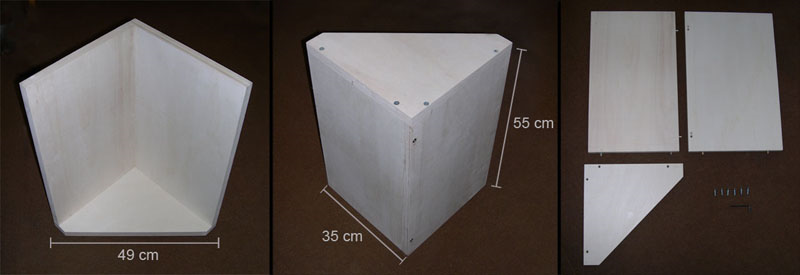
\includegraphics[width=0.9\textwidth]{buildingThreeDCalibrationObject}
\caption{Building \gls{3D} Calibration Object \cite{threeDExample_2014}}
\label{buildingThreeDCalibrationObject}
\end{figure}%
%
\begin{figure}[!t]
\centering
\subfloat[Six Points to Calibrate]{
	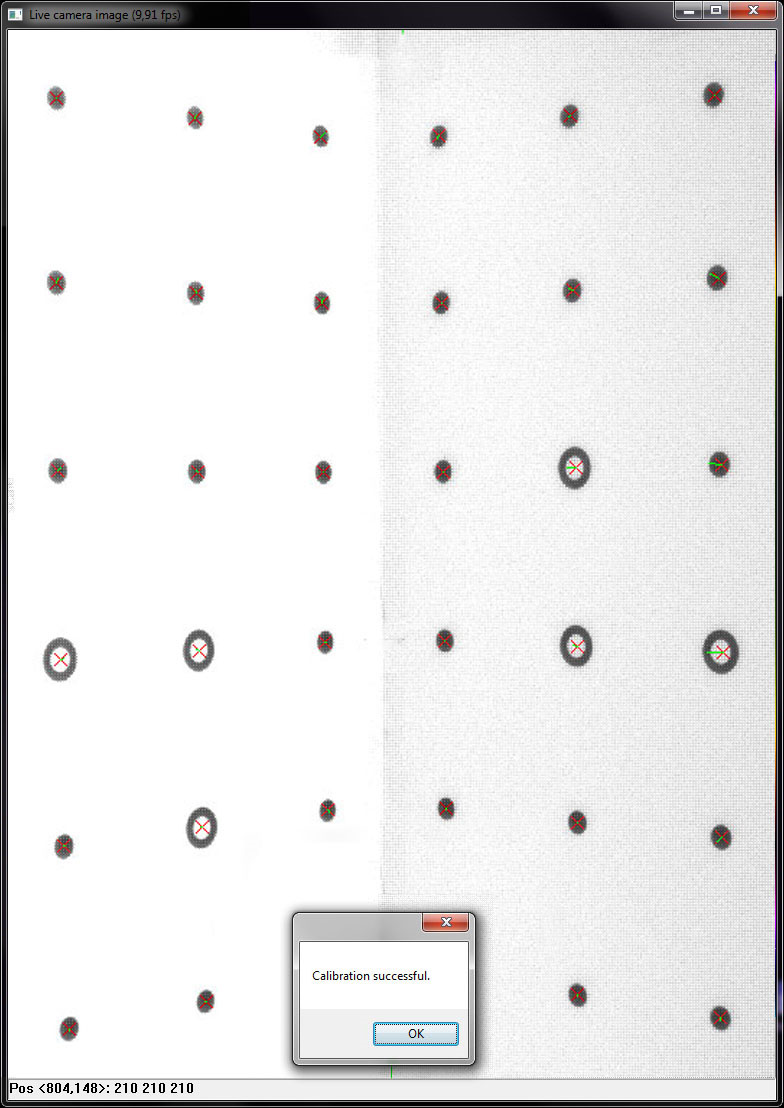
\includegraphics[height=0.6\textwidth, width=0.45\textwidth]{threeDSixPointsCalibrating}
	\label{threeDSixPointsCalibrating}
}
\subfloat[Reconstruction After Calibration]{
	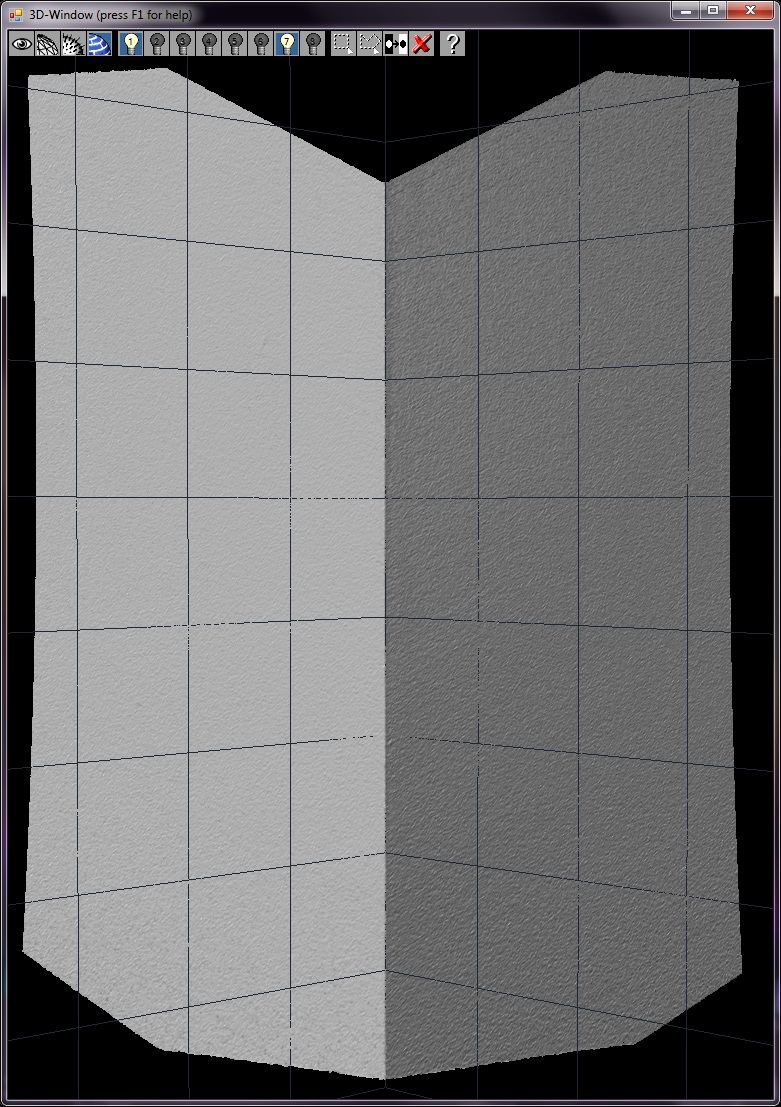
\includegraphics[height=0.6\textwidth, width=0.45\textwidth]{3DreconstructAfterCalibration}
	\label{3DreconstructAfterCalibration}
}
\caption{Three Dimension Object Camera Calibration \cite{threeDExample_2014}}
\label{twoPlanesCalibration}
\end{figure}%
%


%\begin{figure}[p]
%\centering
%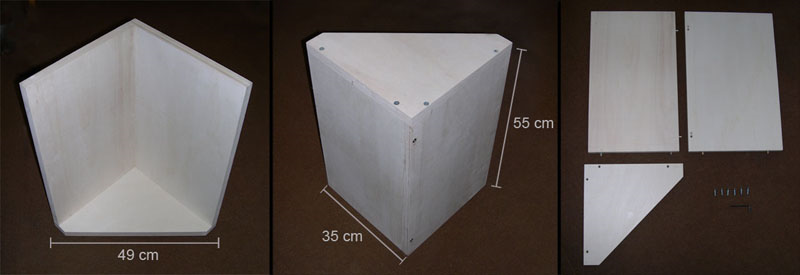
\includegraphics[width=0.8\textwidth]{buildingThreeDCalibrationObject}
%\caption{Building Three Dimension Object}
%\label{buildingThreeDCalibrationObject}
%\end{figure}%
%
%\begin{figure}[b]
%\centering
%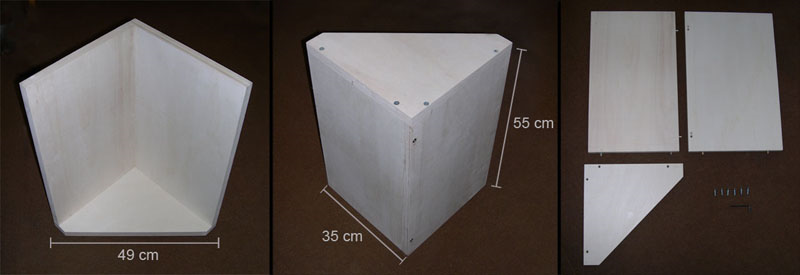
\includegraphics[width=0.8\textwidth]{buildingThreeDCalibrationObject}
%\caption{Building Three Dimension Object}
%\label{buildingThreeDCalibrationObject}
%\end{figure}%




%\\\\%

Zhengyou Zhang \cite{zhangCalibration1_2004, zhangCalibration2_2000, Zhengyou04} has deep studies on camera calibration from one-dimension calibration to tree-dimension calibration. The accuracy of calibration from 1D to \gls{3D} is getting better, but the calibration system set-up needs more and more work and cost as well. One dimension object is suitable for calibrating multiple cameras at once. Two dimension planer pattern approaches seems to be a good compromise, with good accuracy and simple setup. Also using the three dimension method for calibration, Kai \cite{Kai10} derived the per-pixel  beam equation, the linear relationship that could map to \(\gls{worldX}/\gls{worldY}\) from \(\gls{worldZ}\) as eqn.~(\ref{kaiBeamEquation}) shows, directly from pinhole camera matrix \(\gls{pinHoleCameraM}\). That is to say, we could easily look up \(\gls{worldX}/\gls{worldY}\) after calibration once found the way to get \(\gls{worldZ}\).

\begin{equation}
\begin{aligned}
\gls{worldX} [\gls{imDiscreteRow}, \, \gls{imDiscreteColumn}] = a [\gls{imDiscreteRow}, \, \gls{imDiscreteColumn}]  \gls{worldZ} [\gls{imDiscreteRow}, \, \gls{imDiscreteColumn}]+d [\gls{imDiscreteRow}, \, \gls{imDiscreteColumn}] 
\\%
\gls{worldY} [\gls{imDiscreteRow}, \, \gls{imDiscreteColumn}] = c [\gls{imDiscreteRow}, \, \gls{imDiscreteColumn}]  \gls{worldZ} [\gls{imDiscreteRow}, \, \gls{imDiscreteColumn}]+d [\gls{imDiscreteRow}, \, \gls{imDiscreteColumn}] 
\end{aligned}
\label{kaiBeamEquation}
\end{equation}%
\noindent
where \(a/b/c/d\) are per-pixel coefficients for the linear beam equations, and the subscripts \([\gls{imDiscreteRow}, \, \gls{imDiscreteColumn}] \) are corresponding pixel address in image space.

%\gls{D}[r, c] ~= \gls{worldZ}[r, c] -- > (X^c, Y^c)
%\gls{worldZ}[r, c] = Z^c[r, c] = \gls{D}[r,c]

%%%%%%%%%%%%%%%%%%%%%%%%%%%%%%%%%%%%%%%%%%%%%%%%%%%%%
%%%%%%%%%%                                                                                                   %%%%%%%%%%
%%%%%%%%%%      4.        Lens Distortion Removal                                                %%%%%%%%%%%
%%%%%%%%%%                                                                                                    %%%%%%%%%%%
%%%%%%%%%%%%%%%%%%%%%%%%%%%%%%%%%%%%%%%%%%%%%%%%%%%%%%

\section{Lens Distortion}
%* distortion equation
\indent
All above in Chapter \ref{chapterTraditionalCalibration} are talking about the ideal pinhole camera, without lenses. Whereas in practice, as a result of several types of imperfections in the design and assembly of lenses composing the camera optical system, there are always lens distortions for a camera, and the expressions in eqn.~(\ref{twoDRelativeFromCamToIm}) are not valid any more. Lens distortion could be classified into two groups \cite{distortion1_1992} : radial distortion and tangential distortion. Imperfect lens shape causes light rays bending more near the edges of a lens than they do at its optical center. Barrel distortions happen commonly on wide angle lenses, where the field of view of the lens is much wider than the size of the image sensor \cite{whatisDistortion_2013}. Improper lens assembly will lead to tangential distortion, which occurs when the lens and the image plane are not parallel. Figure~\ref{RadialAndTangentialDistortion} shows how radial distortion \(d_\text{r}\) and tangential distortion \(d_\text{t}\) affect the object point position in the image. Note that both of radial distortion and tangential distortion are with respect to image space row and column, and what we will take later is negative distortion instead of positive. Distortions are present because the field of view (\gls{FoV}) in camera space has been affected by the lens. 
%
\begin{figure}[b]
\centering
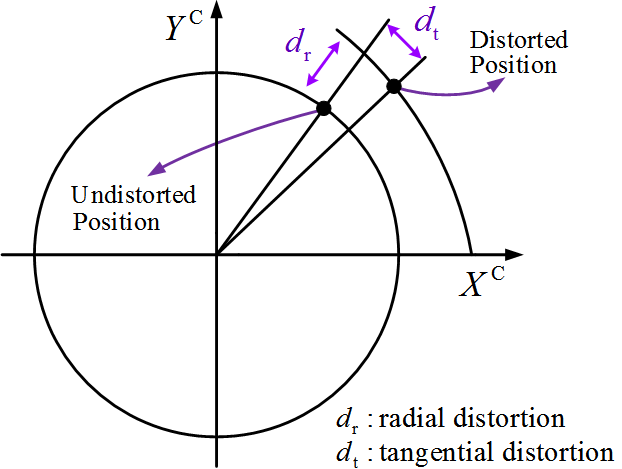
\includegraphics[width=0.65\textwidth]{RadialAndTangentialDistortion}
\caption{Radial and Tangential Distortion Affection In Image Space}
\label{RadialAndTangentialDistortion}
\end{figure}%
%
For most consumer \gls{RGBD} cameras with cheap lens, their distortions are usually barrel distortions (negative distortion) resulted by the enlarged field  of view in the camera space, because the larger view was squeezed into the sensor. Figure~\ref{DistortionComprehension} intuitively shows how the lens enlarged the field of view of in the camera space and then generates the barrel distortions.
%
\begin{figure}[t]
\centering
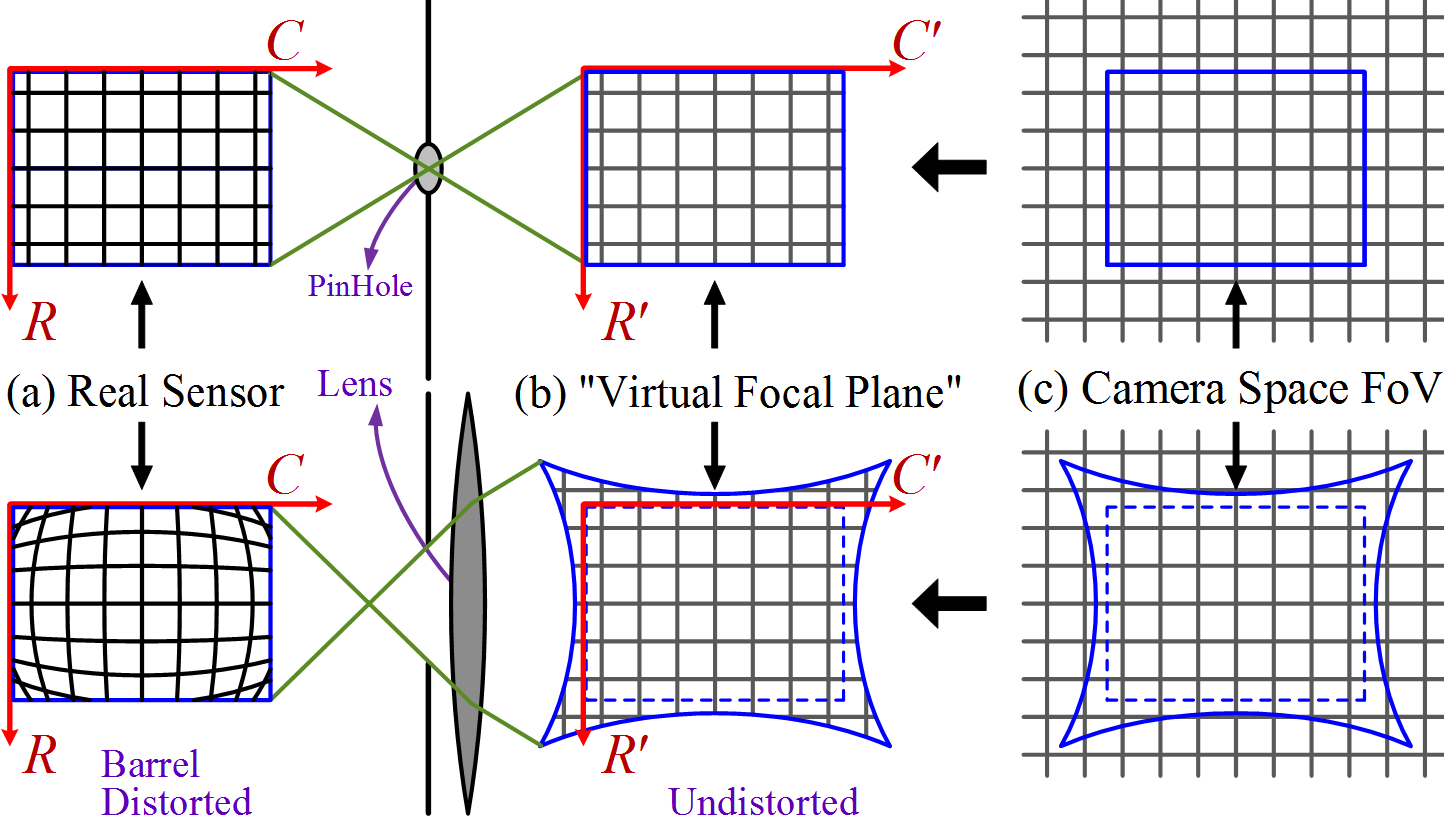
\includegraphics[width=\textwidth]{DistortionComprehension}
\caption{From Camera Space to Image Space with Lens Distortions}
\label{DistortionComprehension}
\end{figure}%

There are (a)(b)(c) three parts shown in Fig.~\ref{DistortionComprehension}. Each part has the pinhole camera only on the top, in contrast to the camera-with-lens situation at the bottom. To understand how the barrel distortion happens, we should go through from part (c) to part (a). In part (c), the gray background uniform grid is the \enquote{object} our that the camera is going to observe, and the blue frames shows the \gls{FoV} of the camera in the camera space. Due to the fact that, there will be worse and worse distortions as one pixel goes from the center to the edge, the enlarged \gls{FoV} of a camera with lens in the camera space is in pincushion (or star) shape. With the enlarged \gls{FoV} is mapped to the \enquote{Virtual Focal Plane}, as defined in Fig.~\ref{PinHoleVirtualFocalPlane}, the pincushion shape doesn't change because rays from the camera space have not gone through the lens yet. Note that we quoted the \enquote{Virtual Focal Plane} because the image on this virtual plane, when considering lens distortion, does not equal to the real focal plane (where the sensor is) any more. We can tell from part (b) that, even though the image space coordinates still are composed of \(\gls{imageColumn}\) and \(\gls{imageRow}\), their ranges have changed from positive integers only to the whole real integers that include negative ones. But the sensor never changes, and so the image space in part (a) still has its range of positive integers. With rays going through the lens, the pincushion-shape \gls{FoV} (the frame in blue) will be squeezed into a small rectangle, and thus we get the image in the real focal plane with its background grid showing a barrel distorted shape. %
%\\\indent%
With lens distortions counted, eqn.~(\ref{twoDRelativeFromCamToIm}) now needs to be changed into 
%
\begin{equation}
\left[ \begin{array}{c} c'_r \\ r'_r \end{array} \right] %
= f %
\left[ \begin{array}{c} \gls{cameraPointX0}/\gls{cameraPointZ0} \\ \gls{cameraPointY0}/\gls{cameraPointZ0} \end{array} \right]%
\label{undistortedRelativeFromCamToIm}
\end{equation}
where \(c'_r\) and \(r'_r\) denote the relative pixel distance on the undistorted \enquote{Virtual Focal Plane}, whose \gls{FoV} is pincushion-shape and image coordinates' ranges include negative integers.%
\\\indent%
Duane \cite{distortion2_1966} gave the lens distortion equation, and the undistorted \(\gls{imageColumn}\) and \(\gls{imageRow}\) (\(C'/R'\) in our notation) can be expressed as power series in radial distance \(r = \sqrt{C^2 + R^2}\):
%
\begin{equation}
\begin{aligned}
\gls{UndistortedImColumn} =  C (1 + k_1 r^2 + k_2 r^4 + k_3 r^6) + [p_1 (r^2 + 2 C^2) + 2 p_2 CR] %
\\
\gls{UndistortedImRow} =  R (1 + k_1 r^2 + k_2 r^4 + k_3 r^6) + [p_2 (r^2 + 2 R^2) + 2 p_1 CR]
\end{aligned}
\label{lensDistortion}
\end{equation}%
%
\noindent
where higher order parameters are omitted for being negligible; \((\gls{UndistortedImColumn} , \, \gls{UndistortedImRow})\) denote the undistorted pixels in the \enquote{Virtual Focal Plane}, \((\gls{imageColumn}, \, \gls{imageRow} )\) denote the distorted pixel in real sensor image, \(k_i\)s are coefficients of radial distortion, and \(p_j\)s are coefficients of tangential distortion. The five parameters \(k_1/k_2/k_3/p_1/p_2\) are usually called distortion parameters. With the distortion parameters calculated, the distorted \((\gls{imageColumn}, \, \gls{imageRow} )\) could be undistorted into \((\gls{UndistortedImColumn} , \, \gls{UndistortedImRow})\), and then \((\gls{UndistortedImColumn} , \, \gls{UndistortedImRow})\) could be used to generate the world space \(\gls{worldX}/\gls{worldY}/\gls{worldZ}\) with intrinsic and extrinsic parameters.
%
%%%%%%%%%%%%%%%%%%%%%%%%%%%%%%%%%%%%%%%%%%%%%%%%%%%%%
%%%%%%%%%%                                                                                                   %%%%%%%%%%
%%%%%%%%%%      4.       Summation                                                                  %%%%%%%%%%%
%%%%%%%%%%                                                                                                    %%%%%%%%%%%
%%%%%%%%%%%%%%%%%%%%%%%%%%%%%%%%%%%%%%%%%%%%%%%%%%%%%%
%\section{Summation}
%%
\indent 
\begin{figure}[t]
\centering
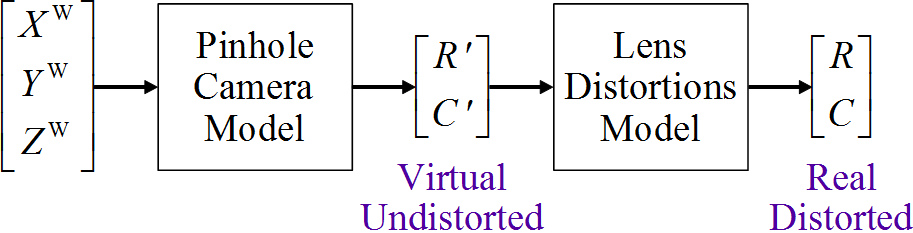
\includegraphics[width=0.6\textwidth]{flowChart}
\caption{Traditional Camera Calibration Flow Chart}
\label{flowChart}
\end{figure}%
\\\indent
Figure~\ref{flowChart} shows the flow chart of the whole traditional camera calibration method based on the pinhole camera model. Considering the lens distortions, both of the pinhole camera model (matrix \(\gls{pinHoleCameraM}\)) and the lens distortions model (five parameters for undistortion) need to be determined. The pinhole camera model can help map from the world space (\(\gls{worldX}, \, \gls{worldY}, \, \gls{worldZ}\)) to the undistorted image space  \((\gls{UndistortedImColumn} , \, \gls{UndistortedImRow})\), which are on the \enquote{Virtual Focal Plane} as noted in Fig.~\ref{DistortionComprehension}. And the lens distortion model help remove the lens distortions by mapping from  \((\gls{UndistortedImColumn} , \, \gls{UndistortedImRow})\) to \((\gls{imageColumn}, \, \gls{imageRow} )\). The pinhole camera model can be determined by eqn.~(\ref{determinationOfPinhole3x4}), and the lens distortion model could be determined by eqn.~(\ref{lensDistortion}).




%
%\begin{equation*}%
%c_{[row, col]} %
%= \frac%
%{(m_{22}m_{33} - m_{23}m_{32})col + (m_{13}m_{32} - m_{12}m_{33})row + (m_{12}m_{23} - m_{13}m_{22})}%
%{(m_{21}m_{32} - m_{22}m_{31})col + (m_{12}m_{31} - m_{11}m_{32})row + (m_{11}m_{22} - m_{12}m_{21})} \, ,
%\end{equation*}
%%
%\begin{equation*}%
%d_{[row, col]} %
%= \frac%
%{(m_{22}m_{34} - m_{24}m_{32})col + (m_{14}m_{32} - m_{12}m_{34})row + (m_{12}m_{24} - m_{14}m_{22})}%
%{(m_{21}m_{32} - m_{22}m_{31})col + (m_{12}m_{31} - m_{11}m_{32})row + (m_{11}m_{22} - m_{12}m_{21})} \, ,
%\end{equation*}
%%
%\begin{equation*}%
%e_{[row, col]} %
%= \frac%
%{(m_{23}m_{31} - m_{21}m_{33})col + (m_{11}m_{33} - m_{13}m_{31})row + (m_{13}m_{21} - m_{11}m_{23})}%
%{(m_{21}m_{32} - m_{22}m_{31})col + (m_{12}m_{31} - m_{11}m_{32})row + (m_{11}m_{22} - m_{12}m_{21})} \, ,
%\end{equation*}
%%
%\begin{equation*}%
%f_{[row, col]} %
%= \frac%
%{(m_{23}m_{32} - m_{22}m_{33})col + (m_{12}m_{33} - m_{13}m_{32})row + (m_{13}m_{22} - m_{12}m_{23})}%
%{(m_{21}m_{32} - m_{22}m_{31})col + (m_{12}m_{31} - m_{11}m_{32})row + (m_{11}m_{22} - m_{12}m_{21})}
%\end{equation*}
%
%



















%Pinhole camera model is wildly used in \gls{3D} camera's reconstruction, however, it is not able to handle non-linear radial distortion. In this chapter, a pinhole model based \gls{3D} camera calibration method (derived from a \gls{3D} reconstruction example of structured light method) will be discussed in detail, and then extended into two newly proposed calibration methods.
%
%%%%%%%%%%%%%%%%%%%%%%%%%%%%%%%%%%%%%%%%%%%%%%%%%%%%%%
%%%%%%%%%%%                                                     %%%%%%%%%%%%%%%%%%%%%%%%%%
%%%%%%%%%%% 2.1   Pinhole Camera Model                   %%%%%%%%%%%%%%%%%%%%%%%%
%%%%%%%%%%%                                                     %%%%%%%%%%%%%%%%%%%%%%%%
%%%%%%%%%%%%%%%%%%%%%%%%%%%%%%%%%%%%%%%%%%%%%%%%%%%%%%%
%
%\section{Pinhole Camera Model}
%\label{sectionPinholeCamera}
%%%
%Fig.~\ref{PinholeCameraModel} shows the basic diagram of a pinhole camera model \cite{Maria10} \cite{Zhengyou04} with a reflected image plane for friendly intuition. From this model, the mapping between \gls{3D} space world coordinate and the image plane row and column could be separated into two parts of transformations. The first part is the transformation between world coordinates system \(X\)/\(Y\)/\(Z\) and camera coordinate system \(U\)/\(V\)/\(W\) , which forms a 4x4 perspective transformation matrix (\textbf{extrinsic calibration}) that works for \gls{3D} rotation and translation. And the second part is the mapping between \gls{3D} camera coordinates system \(U\)/\(V\)/\(W\) and 2D image plane coordinates \(u\)/\(v\), which forms a 3x3 perspective transformation matrix (\textbf{intrinsic calibration}) that works for not only the rescaling between camera coordinates and virtual ideal image coordinates, but also for translating and skewing between the virtual ideal image plane and real image plane. %
%%
%\begin{figure}[h]
%\centering
%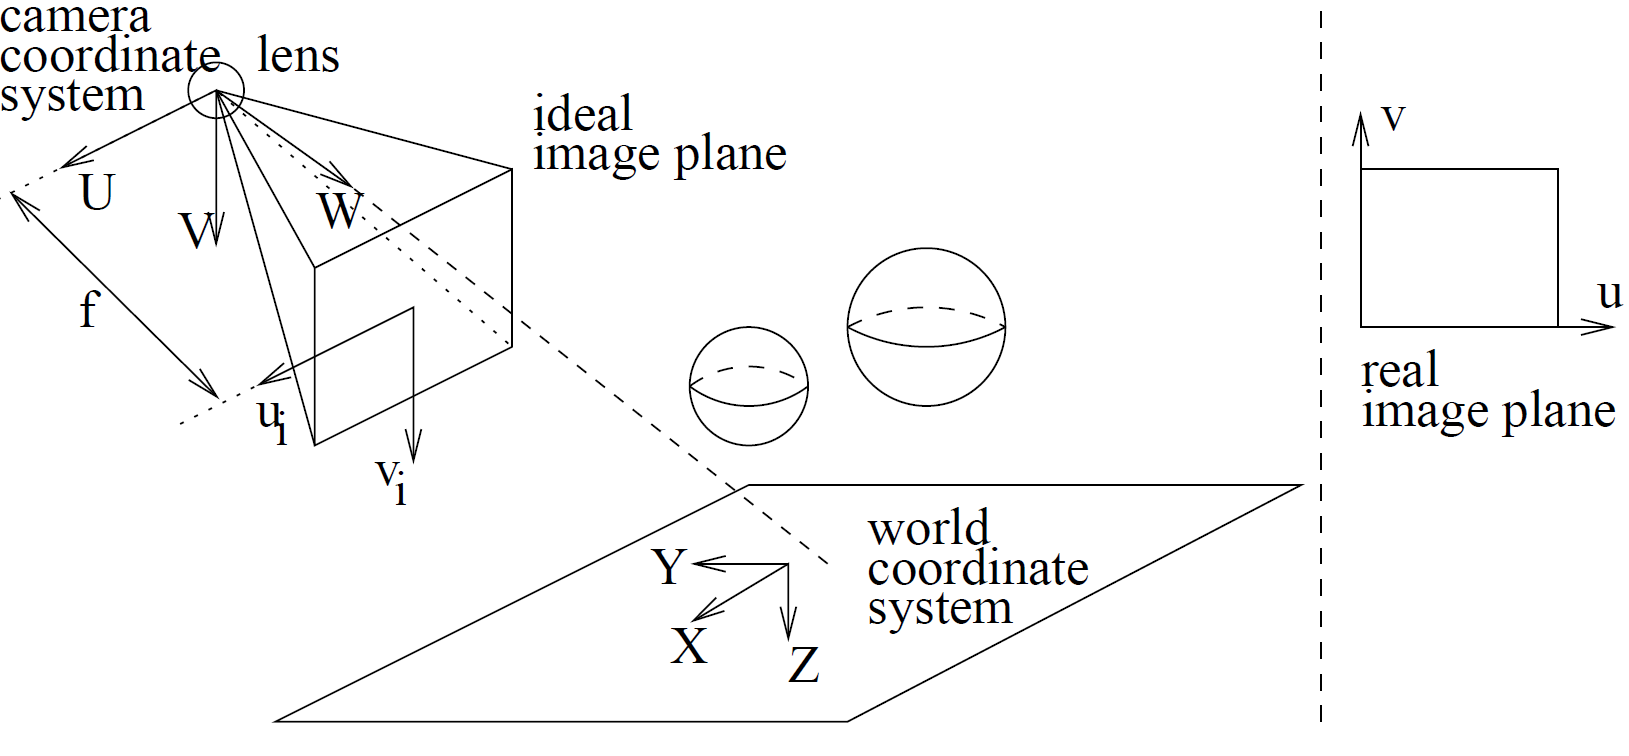
\includegraphics[width=\textwidth]{PinholeCameraModel}
%\caption{The pinhole camera model}
%\label{PinholeCameraModel}
%\end{figure}%
%%
%\\\par%
%\textbf{Extrinsic Calibration}\\
%Without any camera parameters, the extrinsic calibration formula could be written, through homogeneous coordinates, as
%%
%\begin{equation}
%\left[ \begin{array}{c} U \\ V \\ W \\ 1 \end{array} \right] %
%= %
%\begin{bmatrix} R & T \\ 0 & 1 \end{bmatrix} \times \left[ \begin{array}{c} X^w \\ Y^w \\ Z^w \\ 1 \end{array} \right]
%\end{equation}%
%%
%or for simplicity,
%\begin{equation}
%%
%\left[ \begin{array}{c} U \\ V \\ W \end{array} \right] %
%= %
%\begin{bmatrix} R & T \end{bmatrix} \cdot \left[ \begin{array}{c} X^w \\ Y^w \\ Z^w \end{array} \right]
%\label{extrinsicTransform}
%%
%\end{equation}%
%%
%where \((U, V, W)^T\) are the camera coordinates, and the transformation matrix component \([R\)  \(T]\), which is part of the 4x4 perspective matrix, is modeling rotation and translation , written as
%
%\begin{equation}
%%
%\left[ \begin{array}{cc} R & T \end{array} \right] %
%= %
%\begin{bmatrix}
% r_{11} & r_{12} & r_{13} & t_1 \\
% r_{21} & r_{22} & r_{23} & t_2 \\
% r_{31} & r_{32} & r_{33} & t_3
%\end{bmatrix}
%%
%\end{equation}
%\\\par
%%
%%
%\textbf{Intrinsic Calibration}\\
%Intrinsic Calibration could be separated into two sections. The first section is to rescale from camera coordinates to virtual ideal image coordinates. For a easier integration of two sections, the first section's formula is given through both of 2D coordinates to homogeneous coordinates.\par
%%
%\quad\quad2D coordinates:%
%\begin{equation}
%%
%W \left[ \begin{array}{c} u^i \\ v^i  \end{array} \right] %
%= f %
%\left[ \begin{array}{c} U \\ V \end{array} \right]%
%%
%\end{equation}
%
%\quad\quad Homogeneous coordinates:\par
%\begin{equation}
%%
%W \left[ \begin{array}{c} u^i \\ v^i \\ 1 \end{array} \right] %
%= %
%\left[ \begin{array}{c} fU \\ fV \\ W \end{array} \right]%
%=  \begin{bmatrix} f & 0 & 0 \\ 0 & f & 0 \\ 0 & 0 & 1 \end{bmatrix} \cdot %
%\left[ \begin{array}{c} U \\ V \\ W \end{array} \right]%
%\label{section_1}
%\end{equation}%
%\\\par
%%
%The second section is for translating and skewing between the virtual ideal image plane \(u^i\)/\(v^i\) and real image plane \(u^r\)/\(v^r\),  %
%
%\begin{equation}
%%
%\left[ \begin{array}{c} u^r \\ v^r \\ 1 \end{array} \right] %
%=  \begin{bmatrix} s_u & s_\theta & u_0 \\ 0 & s_v & v_0 \\ 0 & 0 & 1 \end{bmatrix} \cdot %
%\left[ \begin{array}{c} u^i \\ v^i \\ 1 \end{array} \right]%
%\label{section_2}
%\end{equation}%
%where \((u_0, v_0)\) denotes the optical center (or principal point), \([s_u, s_v]\) are skew coefficients in pixels along \(u\) and  \(v\) axes , and  \(s_\theta\) is an skewed angle generated by \(s_u\) and  \(s_v\). To combine eqn.~\ref{section_1} and eqn.~\ref{section_2}, we could get %
%
%\begin{equation}
%%
%W \left[ \begin{array}{c} u^r \\ v^r \\ 1 \end{array} \right] %
%=  \begin{bmatrix} s_u & s_\theta & u_0 \\ 0 & s_v & v_0 \\ 0 & 0 & 1 \end{bmatrix} \cdot%
% \begin{bmatrix} f & 0 & 0 \\ 0 & f & 0 \\ 0 & 0 & 1 \end{bmatrix} \cdot %
%\left[ \begin{array}{c} U \\ V \\ W \end{array} \right]%
%=  \begin{bmatrix} f_u & s & u_0 \\ 0 & f_v & v_0 \\ 0 & 0 & 1 \end{bmatrix} \cdot%
%\left[ \begin{array}{c} U \\ V \\ W \end{array} \right]%
%%
%\label{intrinsicTransform}
%\end{equation}%
%%
%where \([f_u,\, f_v]\) denote focal lengths in pixels along \(u\) and \(v\) after skewing, and \(s\) is a new skew coefficient after combination.\\\par%
%%
%\textbf{Generic Perspective Matrix of the Pinhole Camera Model}\par%
%
%After both of the extrinsic and intrinsic transformation matrices have been derived, the generalization formula of the pinhole camera model could be derived, combining eqn.~\ref{extrinsicTransform} and \ref{intrinsicTransform}, as
%
%\begin{equation}
%%
%k \left[ \begin{array}{c} u^r \\ v^r \\ 1 \end{array} \right] %
%=  \begin{bmatrix} f_u & s & u_0 \\ 0 & f_v & v_0 \\ 0 & 0 & 1 \end{bmatrix} \cdot%
%\begin{bmatrix} R & T \end{bmatrix} \cdot \left[ \begin{array}{c} X^w \\ Y^w \\ Z^w \\ 1 \end{array} \right]%
%=  C \cdot \left[ \begin{array}{c} X^w \\ Y^w \\ Z^w \\ 1 \end{array} \right]%
%%
%\label{detailedPerspectivePinholeCameraMatrix}
%\end{equation}%
%%
%where \(W\) on the left side has been replaced by \(k\) to be a more general proportion coefficient, and a combined matrix can be expressed as
%\begin{equation}
%%
%C %
%=  \begin{bmatrix} f_u & s & u_0 \\ 0 & f_v & v_0 \\ 0 & 0 & 1 \end{bmatrix} \cdot%
%\begin{bmatrix} R & T \end{bmatrix}%
%= \begin{bmatrix} 
%m_{11} & m_{12} & m_{13} & m_{14} \\
%m_{21} & m_{22} & m_{23} & m_{24} \\
%m_{31} & m_{32} & m_{33} & m_{34} \\
%\end{bmatrix}%
%%
%\label{genericPerspectivePinholeMatrix}
%\end{equation}%
%%
%The final $3\times4$ matrix C is considered as the generic perspective transformation matrix of a pinhole camera model, which gives a mapping between the \gls{3D} world coordinates and 2D real image coordinates. To inspect the pinhole camera matrix, its effects focuses on the taking care of linear processes of rotation, translation and skewing, given a perspective view. In other words, this $3\times4$ transformation matrix is specially for the removal perspective distortion . It is based on the homogeneous coordinates, while also limited by the linear system. And a mapping using this $3\times4$ transformation matrix between two coordinates can only be linear.
%\\\\%
%The pinhole camera matrix can be solved using least squares fit with known \gls{3D} points (\(X^w\), \(Y^w\), \(Z^w\)) and their corresponding image points (\(u^r\), \(v^r\)). With one point, based on eqn.~\ref{detailedPerspectivePinholeCameraMatrix} and \ref{genericPerspectivePinholeMatrix}, we can get
%\begin{equation}
%\begin{aligned}
%m_{11}X^w + m_{12}Y^w + m_{13}Z^w + m_{14} - m_{31}u^rX^w - m_{32}u^rY^w - m_{33}u^rZ^w - m_{34}u^r = 0%
%\\%
%m_{21}X^w + m_{22}Y^w + m_{23}Z^w + m_{24} - m_{31}v^rX^w - m_{32}v^rY^w - m_{33}v^rZ^w - m_{34}v^r = 0
%\end{aligned}
%\label{onePointEquationCR}
%\end{equation}%
%There are two equations for one point, and totally 12 unknowns to solve. We need at least six points to solve the $3\times4$ pinhole camera matrix. Using n-points least squares to solve the best fit, we can build a 2n equations matrix
%
%\begin{equation}
%\hspace*{-1cm}
%\begin{bmatrix} 
%X^w_1 & Y^w_1 & Z^w_1 & 1 & 0 & 0 & 0 & 0 & -u^r_1X^w_1 & -u^r_1Y^w_1 & -u^r_1Z^w_1 & -u^r_1\\
%0 & 0 & 0 & 0 & X^w_1 & Y^w_1 & Z^w_1 & 1 &  -v^r_1X^w_1 & -v^r_1Y^w_1 & -v^r_1Z^w_1 & -v^r_1\\
%X^w_2 & Y^w_2 & Z^w_2 & 1 & 0 & 0 & 0 & 0 & -u^r_2X^w_2 & -u^r_2Y^w_2 & -u^r_2Z^w_2 & -u^r_2\\
%0 & 0 & 0 & 0 & X^w_2 & Y^w_2 & Z^w_2 & 1 &  -v^r_2X^w_2 & -v^r_2Y^w_2 & -v^r_2Z^w_2 & -v^r_2\\
% & & & & & & & \vdots & & & & \\
%X^w_n & Y^w_n & Z^n_2 & 1 & 0 & 0 & 0 & 0 & -u^r_nX^w_n & -u^r_nY^w_n & -u^r_nZ^w_n & -u^r_n\\
%0 & 0 & 0 & 0 & X^w_n & Y^w_n & Z^w_n & 1 & -v^r_nX^w_n & -v^r_nY^w_n & -v^r_nZ^w_n & -v^r_n
%\end{bmatrix}
%\begin{bmatrix} 
%m_{11} \\ m_{12} \\ m_{13} \\ m_{14} \\
%m_{21} \\ m_{22} \\ m_{23} \\ m_{24} \\
%m_{31} \\ m_{32} \\ m_{33} \\ m_{34} 
%\end{bmatrix}
%=
%\begin{bmatrix} 
%0 \\ 0 \\ 0 \\ 0 \\
%\vdots \\ 0 \\ 0
%\end{bmatrix}
%\label{nPoints2nEquationCR}
%\end{equation}%
%
%
%Considering that this matrix is build on homogeneous system, there is no unique solution. There can always be a total-zeros solution. To make the solution unique, we select \(m_{34} = 1\), so that the homogeneous eqn.~\ref{nPoints2nEquationCR} could be changed into an inhomogeneous format like \(AX = B\), as eqn.~\ref{inHomogenousNPoints2nEquationCR} below.
%
%\begin{equation}
%\hspace*{-0.1cm}
%\begin{bmatrix} 
%X^w_1 & Y^w_1 & Z^w_1 & 1 & 0 & 0 & 0 & 0 & -u^r_1X^w_1 & -u^r_1Y^w_1 & -u^r_1Z^w_1\\
%0 & 0 & 0 & 0 & X^w_1 & Y^w_1 & Z^w_1 & 1 &  -v^r_1X^w_1 & -v^r_1Y^w_1 & -v^r_1Z^w_1\\
%X^w_2 & Y^w_2 & Z^w_2 & 1 & 0 & 0 & 0 & 0 & -u^r_2X^w_2 & -u^r_2Y^w_2 & -u^r_2Z^w_2\\
%0 & 0 & 0 & 0 & X^w_2 & Y^w_2 & Z^w_2 & 1 &  -v^r_2X^w_2 & -v^r_2Y^w_2 & -v^r_2Z^w_2\\
% & & & & & & & \vdots & & &\\
%X^w_n & Y^w_n & Z^n_2 & 1 & 0 & 0 & 0 & 0 & -u^r_nX^w_n & -u^r_nY^w_n & -u^r_nZ^w_n\\
%0 & 0 & 0 & 0 & X^w_n & Y^w_n & Z^w_n & 1 & -v^r_nX^w_n & -v^r_nY^w_n & -v^r_nZ^w_n
%\end{bmatrix}
%\begin{bmatrix} 
%m_{11} \\ m_{12} \\ m_{13} \\ m_{14} \\
%m_{21} \\ m_{22} \\ m_{23} \\ m_{24} \\
%m_{31} \\ m_{32} \\ m_{33}
%\end{bmatrix}
%=
%\begin{bmatrix} 
%u^r_1 \\ v^r_1 \\ u^r_2 \\ v^r_2 \\
%\vdots \\ u^r_n \\ v^r_n
%\end{bmatrix}
%\label{inHomogenousNPoints2nEquationCR}
%\end{equation}%
%
%Using pseudo inverse, eqn.~\ref{inHomogenousNPoints2nEquationCR} can be solved by \(X = (A^TA)^{-1}A^TB\), where \(X\) is an 11-elements vector and \(X(1)\)  \texttildelow \, \(X(11)\) correspond to \(m_{11}\) \texttildelow \, \(m_{33}\). And the $3\times4$ pinhole camera matrix, eqn.~\ref{genericPerspectivePinholeMatrix}, will be determined as
%
%\begin{equation}
%C =
%\begin{bmatrix} 
%X(1) & X(2) & X(3) & X(4) \\
%X(5) & X(6) & X(7) & X(8) \\
%X(9) & X(10) & X(11) & 1
%\end{bmatrix}
%\label{determinationOfPinhole3x4}
%\end{equation}%
%

%%%%%%%%%%%%%%%%%%%%%%%%%%%%%%%%%%%%%%%%%%%%%%%%%%%%%%%
%%%%%%%%%%                                                                              %%%%%%%%%%%%%%%%%%%%%
%%%%%%%%%% 2.2   Structured Light \gls{3D} Reconstruction in Real-Time   %%%%%%%%%%%%%%%%%%%
%%%%%%%%%%                                                                                 %%%%%%%%%%%%%
%%%%%%%%%%%%%%%%%%%%%%%%%%%%%%%%%%%%%%%%%%%%%%%%%%%%%
%\section{Structured Light \gls{3D} Reconstruction in Real-Time}
%\label{sectionSL3DReconstructionRealTime}
%Using a \gls{3D} reconstruction method of structured light, applying Phase Measuring Profilometry (PMP) technique, a per-pixel \gls{3D} camera calibration method based on pinhole camera model is detailedly introduced in this section. Both of the advantage and disadvantage are discussed.
%%
%%
%\begin{figure}[H]
%\centering
%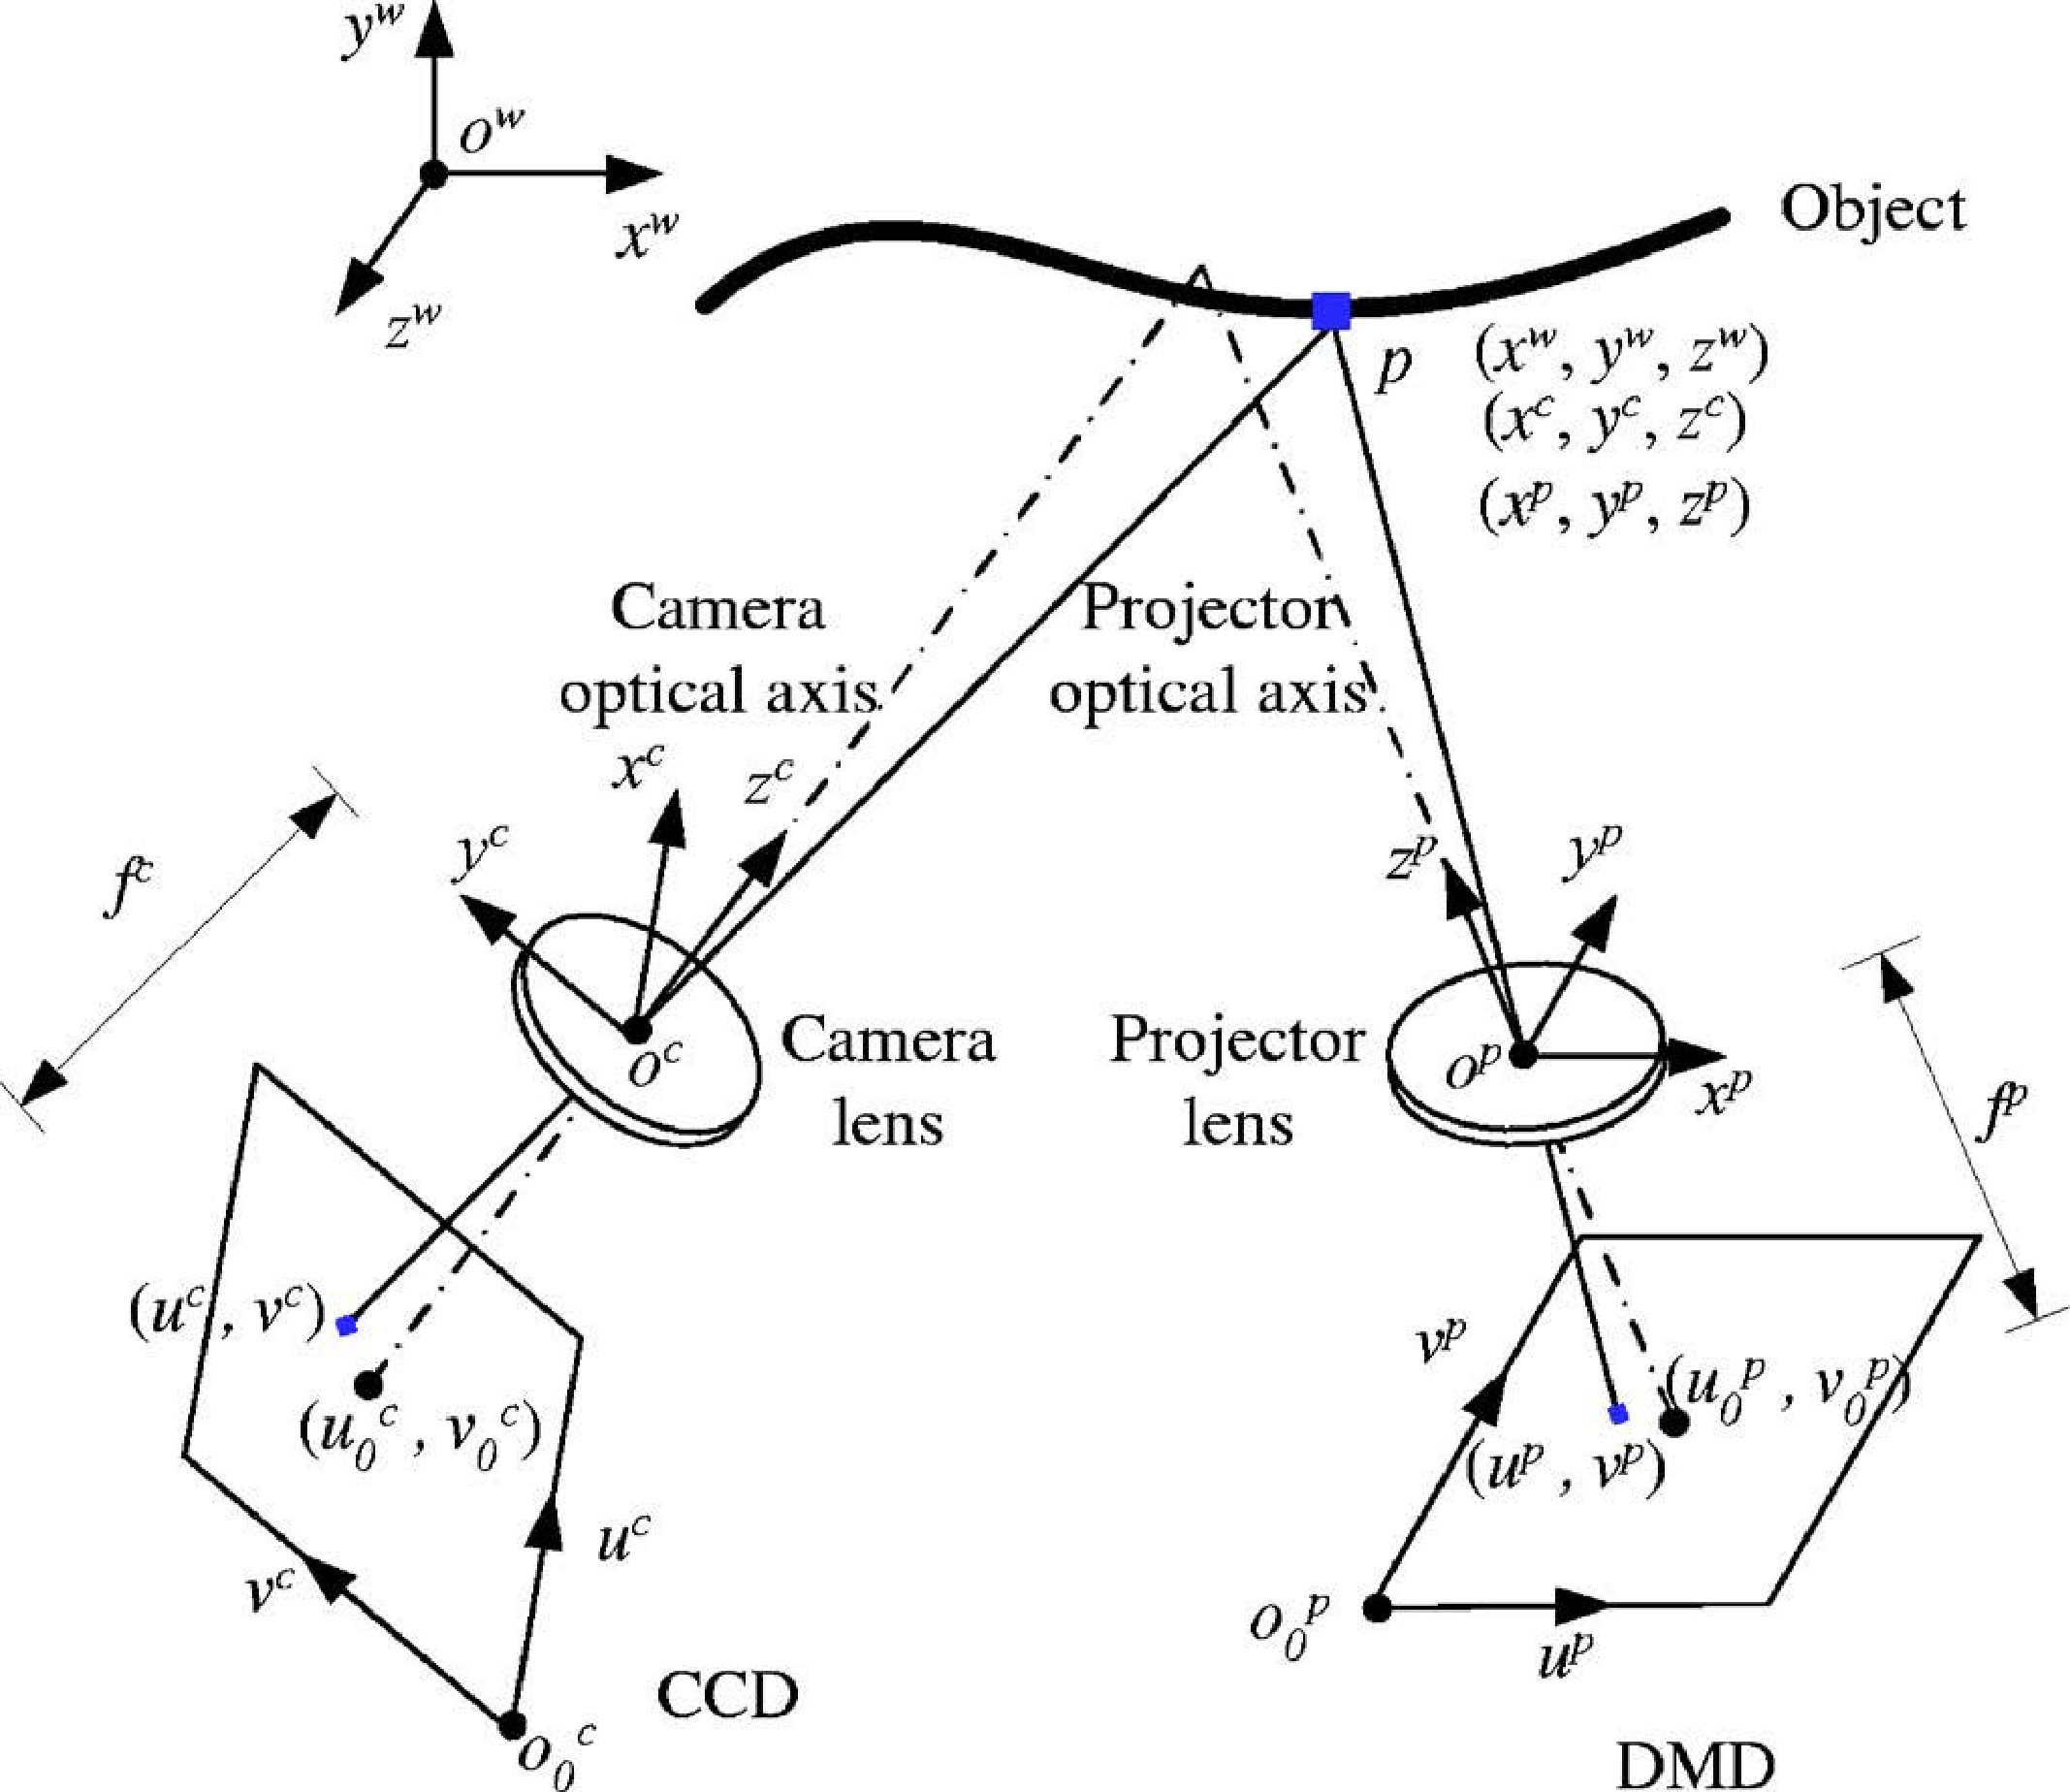
\includegraphics[width=0.7\textwidth]{SLPMPConfiguration}
%\caption{SL PMP Configuration Diagram \cite{Song06}}
%\label{SLPMPConfiguration}
%\end{figure}%
%%
%A \gls{3D} shape measurement system consists of a Charge-Coupled Device (CCD) camera and a Digital Micro-mirror Device (DMD) projector. 2D image pattern strategies are always preferred for fast scanning if a DMD projector is involved
%[**]%J. Salvi, J. Pages, and J. Batlle, \Pattern codication strategies in structured light systems," Pattern Recognition 37, 827{849 (2004).
% \cite{Song06}.
%And the multi-shot pattern Phase Measuring Profilometry strategy was used for its properties of robust and accuracy.
%With PMP information encoded in the structured light pattern projected onto the target, the CCD camera could capture a series of images that contains PMP informatio. Triangulation analyzing could be used to extract the \gls{3D} world coordinates for each points of the target profile, by a determination of the relationships among CCD camera, DMD projector, and the target object. A system configuration of PMP application is given in Fig.~\ref{SLPMPConfiguration}.%
%\\\\%
%PMP method uses either vertical or horizontal sinusoid patterns, which could be described as:
%
% \begin{equation}
%%
%I^p_n(x^p, \, y^p) %
%= A^p(x^p, \, y^p) + B^p(x^p, \, y^p)Cos(2\pi fy^p - \frac{2\pi n}{N})
%%
%\end{equation}%
%%
%where \((x^p, \, y^p)\) denotes the coordinates of every single pixel in the projector, \(I^p_n\) denotes the intensity of the corresponding pixels, \(A^p\) and \(B^p\) are constants, \(f\) is the frequency of sine wave. The subscript \(n\) represents the index of phase shift, while capital \(N\) is the total number of phase shift.\par%
%%
%%
% \begin{figure}[h]
%%\centering
%\hspace*{-2cm} 
%\subfloat[Pattern 0][1]{
%
\includegraphics[width=0.3\textwidth]{Pattern0}
%\label{fig:subfig1}}
%\subfloat[Pattern 1][2]{
%
\includegraphics[width=0.3\textwidth]{Pattern1}
%\label{fig:subfig2}}
%\subfloat[Pattern 2][3]{
%
\includegraphics[width=0.3\textwidth]{Pattern2}
%\label{fig:subfig3}}
%%\qquad
%\subfloat[Pattern 3][4]{
%
\includegraphics[width=0.3\textwidth]{Pattern3}
%\label{fig:subfig4}}
%\caption{PMP base frequency patterns}
%\label{PMPFrequencyPatterns}
%\end{figure}%
%%
%%\begin{figure}
%%    \centering
%%    \hspace*{-3cm} 
%%    \begin{subfigure}[b]{0.3\textwidth}
%%            
\includegraphics[width=\textwidth]{Pattern0}
%%            \caption{Pattern 0}
%%    \end{subfigure}%
%%    ~ 
%%    \begin{subfigure}[b]{0.3\textwidth}
%%            
\includegraphics[width=\textwidth]{Pattern1}
%%            \caption{Pattern 1}
%%    \end{subfigure}
%%    ~ 
%%    \begin{subfigure}[b]{0.3\textwidth}
%%            
\includegraphics[width=\textwidth]{Pattern2}
%%            \caption{Pattern 2}
%%    \end{subfigure}
%%    ~ 
%%    \begin{subfigure}[b]{0.3\textwidth}
%%            
\includegraphics[width=\textwidth]{Pattern3}
%%            \caption{Pattern 3}
%%    \end{subfigure}
%%    \caption{PMP base frequency patterns}
%%    \label{PMPFrequencyPatterns}
%%\end{figure}
%%
%%
%%
%Fig.~\ref{PMPFrequencyPatterns} shows a group of sine wave patterns, where the number of total phase shift \(N = 4\) and frequency \(f = 1\). From viewpoint of the camera, the sinusoid patterns is distorted by the target surface topology, so that the captured images could be expressed as 
%
% \begin{equation}
%%
%I^c_n(x^c, \, y^c) %
%= A^c(x^c, \, y^c) + B^c(x^c, \, y^c)Cos[\phi(x^c,\, y^c) - \frac{2\pi n}{N}]
%%
%\end{equation}%
%%
%where\((x^c, \, y^c)\) denotes the coordinates of every single pixel in the camera, and the term \(\phi(x^c,\, y^c)\) represents the corresponding phase value, which could be computed as follows [6]\par
% % Very High Resolution 3D surface Scanning Using Multi-Frequency Phase Measuring Profilometry
% \begin{equation}
%%
%\phi(x^c,\, y^c) %
%= arctan\Bigg[\frac{\sum^N_{n=1}I(x^c,\,y^c)Sin(2\pi n / N)}{\sum^N_{n=1}I(x^c,\,y^c)Cos(2\pi n / N)} \Bigg]
%%
%\label{equationArctangent}
%\end{equation}
%%
%%
%After the camera term  \(\phi(x^c,\, y^c)\)  for every single pixel is computed, the corresponding projector coordinate \(y^p\) could be derived through equation\par
%
%\begin{equation}
%%
%y^p %
%= \phi(x^c,\, y^c) / (2\pi f)
%%
%\end{equation}%
%%
%With the knowledge of \(y^p\), the perspective information between camera and projector is the last step to go for applying triangulation analysis to extract world coordinates. Based on pinhole camera model, the perspective matrices for both of the CCD camera and DMD projector, as will be derived later in section \ref{sectionPinholeCamera} eqn.~\ref{genericPerspectivePinholeMatrix}, are written as [7]\par
%% J. Li, L. G. Hassebrook, and C. Guan, \Optimized two-frequency phasemeasuring-prolometry light-sensor temporal-noise sensitivity," Journal of the Optical Society of America A 20, 106{115 (2003).
%
%\begin{equation}
%%
%M^c %
%= \begin{bmatrix} 
%m^c_{11} & m^c_{12} & m^c_{13} & m^c_{14} \\
%m^c_{21} & m^c_{22} & m^c_{23} & m^c_{24} \\
%m^c_{31} & m^c_{32} & m^c_{33} & m^c_{34} \\
%\end{bmatrix}%
%%
%%\label{genericPerspectivePinholeMatrix}
%\end{equation}%
%%
%and 
%
%\begin{equation}
%%
%M^p %
%= \begin{bmatrix} 
%m^p_{11} & m^p_{12} & m^p_{13} & m^p_{14} \\
%m^p_{21} & m^p_{22} & m^p_{23} & m^p_{24} \\
%m^p_{31} & m^p_{32} & m^p_{33} & m^p_{34} \\
%\end{bmatrix}%
%%
%%\label{genericPerspectivePinholeMatrix}
%\end{equation}%
%%
%The mapping from \gls{3D} world coordinates to 2D camera coordinates are given by\par
%
%\begin{equation}
%%
%x^c %
%= \frac%
%{m^c_{11}X^w + m^c_{12}Y^w + m^c_{13}Z^w + m^c_{14}}%
%{m^c_{31}X^w + m^c_{32}Y^w + m^c_{33}Z^w + m^c_{34}}
%%
%\label{cameraXmapping}
%\end{equation}%
%%
%%
%\begin{equation}
%%
%y^c %
%= \frac%
%{m^c_{21}X^w + m^c_{22}Y^w + m^c_{23}Z^w + m^c_{24}}%
%{m^c_{31}X^w + m^c_{32}Y^w + m^c_{33}Z^w + m^c_{34}}
%%
%\label{cameraYmapping}
%\end{equation}%
%%
%%
%Likewise, the translation from \gls{3D} world coordinates to 2D projector coordinates are given by\par
%\begin{equation}
%%
%x^p %
%= \frac%
%{m^p_{11}X^w + m^p_{12}Y^w + m^p_{13}Z^w + m^p_{14}}%
%{m^p_{31}X^w + m^p_{32}Y^w + m^p_{33}Z^w + m^p_{34}}
%%
%\label{projectorXmapping}
%\end{equation}%
%%
%\begin{equation}
%%
%y^p %
%= \frac%
%{m^p_{21}X^w + m^p_{22}Y^w + m^p_{23}Z^w + m^p_{24}}%
%{m^p_{31}X^w + m^p_{32}Y^w + m^p_{33}Z^w + m^p_{34}}
%%
%\label{projectorYmapping}
%\end{equation}%
%%
%%
%Since three out of four equations \ref{cameraXmapping} \texttildelow \,\ref{projectorYmapping} are enough to solve \(X^{w}\),  \(Y^{w}\),  and \(Z^{w}\), and \(y^p\) is already calculated, the \gls{3D} world coordinates \(X^{w}\)/\(Y^{w}\)/\(Z^{w}\)  could be derived from Eqs  \ref{cameraXmapping},  \ref{cameraYmapping}, and \ref{projectorYmapping}\par%
%%
%\begin{equation}
%\hspace*{-0.3cm} 
%%
%\left[ \begin{array}{c} X^w\\ Y^w\\ Z^w\end{array} \right] %
%= %
%\begin{bmatrix} %
%m^c_{11} - m^c_{31}x^c, &m^c_{12} - m^c_{32}x^c, &m^c_{13} - m^c_{33}x^c \\%
%m^c_{21} - m^c_{31}y^c, &m^c_{22} - m^c_{32}y^c, &m^c_{23} - m^c_{33}y^c \\%
%m^p_{21} - m^p_{31}y^p, &m^p_{22} - m^p_{32}y^p, &m^p_{23} - m^p_{33}y^p %
%\end{bmatrix} ^{-1} %
%\left[ \begin{array}{c}%
%m^c_{34}y^c - m^c_{14}\\%
%m^c_{34}y^c - m^c_{24}\\%
%m^p_{34}y^p - m^p_{24}%
%\end{array} \right]
%%
%\label{equationInversion}
%\end{equation}%
%\\\\%
%%
%
%Traditionally, as derived above, it is the arctangent computation (eqn.~\ref{equationArctangent}) and the matrix inversion (eqn.~\ref{equationInversion}) that prove to be the bottleneck, preventing real-time surface reconstruction. However, Kai proposed a \gls{LUT}-based solution that solves the bottleneck by expanding those two equations into new forms, directly building accurate LUTs. Based on Kai's derivation \cite{Kai10}, \(X^{w}\) and \(Y^{w}\) can be computed respectively as 
%%
%\begin{equation}
%X^w_{(col^c, \, row^c)} = c_{(col^c, row^c)}Z^w_{(col^c, \, row^c)}+d_{(col^c, row^c)}
%\label{equationLUT_X}
%\end{equation}%
%and %
%\begin{equation}
%Y^w_{(col^c, \, row^c)} = e_{(col^c, row^c)}Z^w_{(col^c, \, row^c)}+f_{(col^c, row^c)}
%\label{equationLUT_Y}
%\end{equation}
%%
%where 
%%
%\begin{equation*}%
%c_{(col^c, row^c)} %
%= \frac%
%{(m^c_{22}m^c_{33} - m^c_{23}m^c_{32})col^c + (m^c_{13}m^c_{32} - m^c_{12}m^c_{33})row^c + (m^c_{12}m^c_{23} - m^c_{13}m^c_{22})}%
%{(m^c_{21}m^c_{32} - m^c_{22}m^c_{31})col^c + (m^c_{12}m^c_{31} - m^c_{11}m^c_{32})row^c + (m^c_{11}m^c_{22} - m^c_{12}m^c_{21})} \, ,
%\end{equation*}
%%
%\begin{equation*}%
%d_{(col^c, row^c)} %
%= \frac%
%{(m^c_{22}m^c_{34} - m^c_{24}m^c_{32})col^c + (m^c_{14}m^c_{32} - m^c_{12}m^c_{34})row^c + (m^c_{12}m^c_{24} - m^c_{14}m^c_{22})}%
%{(m^c_{21}m^c_{32} - m^c_{22}m^c_{31})col^c + (m^c_{12}m^c_{31} - m^c_{11}m^c_{32})row^c + (m^c_{11}m^c_{22} - m^c_{12}m^c_{21})} \, ,
%\end{equation*}
%%
%\begin{equation*}%
%e_{(col^c, row^c)} %
%= \frac%
%{(m^c_{23}m^c_{31} - m^c_{21}m^c_{33})col^c + (m^c_{11}m^c_{33} - m^c_{13}m^c_{31})row^c + (m^c_{13}m^c_{21} - m^c_{11}m^c_{23})}%
%{(m^c_{21}m^c_{32} - m^c_{22}m^c_{31})col^c + (m^c_{12}m^c_{31} - m^c_{11}m^c_{32})row^c + (m^c_{11}m^c_{22} - m^c_{12}m^c_{21})} \, ,
%\end{equation*}
%%
%\begin{equation*}%
%f_{(col^c, row^c)} %
%= \frac%
%{(m^c_{23}m^c_{32} - m^c_{22}m^c_{33})col^c + (m^c_{12}m^c_{33} - m^c_{13}m^c_{32})row^c + (m^c_{13}m^c_{22} - m^c_{12}m^c_{23})}%
%{(m^c_{21}m^c_{32} - m^c_{22}m^c_{31})col^c + (m^c_{12}m^c_{31} - m^c_{11}m^c_{32})row^c + (m^c_{11}m^c_{22} - m^c_{12}m^c_{21})}
%\end{equation*}
%%
%and (\(col^c, \, row^c\)) denote the address of a camera's pixel, \(c\)/\(d\)/\(e\)/\(f\) are the corresponding linear coefficients that help map from \(Z^w\) to \(X^w\) and \(Y^w\).%
%\\\\%
%After Kai's expansion from equation eqn.~\ref{equationInversion} to eqn.~\ref{equationLUT_X} and \ref{equationLUT_Y}, the parameters of the projector's pinhole camera matrix are gone, and everything left belongs to the camera (with superscript of \(c\)). It means that, for arbitrary \gls{RGBD} \gls{3D} camera, its calibration could be done by acquiring its 3-by-4 pinhole camera matrix, and then generating beam equations of \ref{equationInversion} and \ref{equationLUT_X} for every single pixel.
%%
%%%%%%%%%%%%%%%%%%%%%%%%%%%%%%%%%%%%%%%%%%%%%%%%%%
%%%%%%%%%%%                                                                       %%%%%%%%%%%%%
%%%%%%%%%%%        3.3  Shortcoming and Extension                  %%%%%%%%%%%%%%%%%%%
%%%%%%%%%%%                                                                                 %%%%%%%%%%%%%
%%%%%%%%%%%%%%%%%%%%%%%%%%%%%%%%%%%%%%%%%%%%%%%%%%%%%%
%\section{Shortcoming and Extension}
%\subsection{Shortcoming}
%The camera calibration method discussed in section \ref{sectionSL3DReconstructionRealTime} is totally derived from the pinhole camera model, which gives the relationship from \(Z^w\) to \(X^w\) and \(Y^w\), and the 2D mapping from \(u^r\)/\(v^r\) (\(\gls{imageColumn}\)/\(\gls{imageRow}\)) to \(X^w\)/\(Y^w\), as Fig.~\ref{PinholeCameraModel} shows. And eqn.~\ref{genericPerspectivePinholeMatrix} and \ref{detailedPerspectivePinholeCameraMatrix} tell us that, the pinhole matrix can only handle linear transformation, i.e., the calibration exclusively based on the pinhole camera model can only handle perspective distortions, whereas the most important radial dominated non-linear lens distortions still exist inside \(X^w\) and \(Y^w\).%
%%
%\\\\%

%%%%%%%%%%%%%%
%%%%%%%%%%%%%%
%%%%%%%%%%%%%%
%%%%%%%%%%%%%%
%\subsection{Extended Method One}
%Although the 3-by-4 pinhole camera matrix is not helpful for removing lens distortion, the pinhole camera model is still a good model that can help determining the relationship from \(Z^w\) to \(X^w\) and \(Y^w\), and that is exactly what a \gls{3D} camera calibration needs for determining the beam equation for every single pixel.%
%\\\\%
%Fig.~\ref{CaliPinHolCameraModel} shows the lens distortion removed pinhole camera model. In this model, the coordinates-pairs (\(\gls{imageColumn}\) / \(\gls{imageRow}\) and \(X^w\)/\(Y^w\)), which was used to train the 3-by-4 pinhole matrix, are now used to train a high order polynomial transformation matrix. The orange pillow shape shows the lens distortion removed image, which was a rectangle in blue.
%%
%\begin{figure}[H]
%\centering
%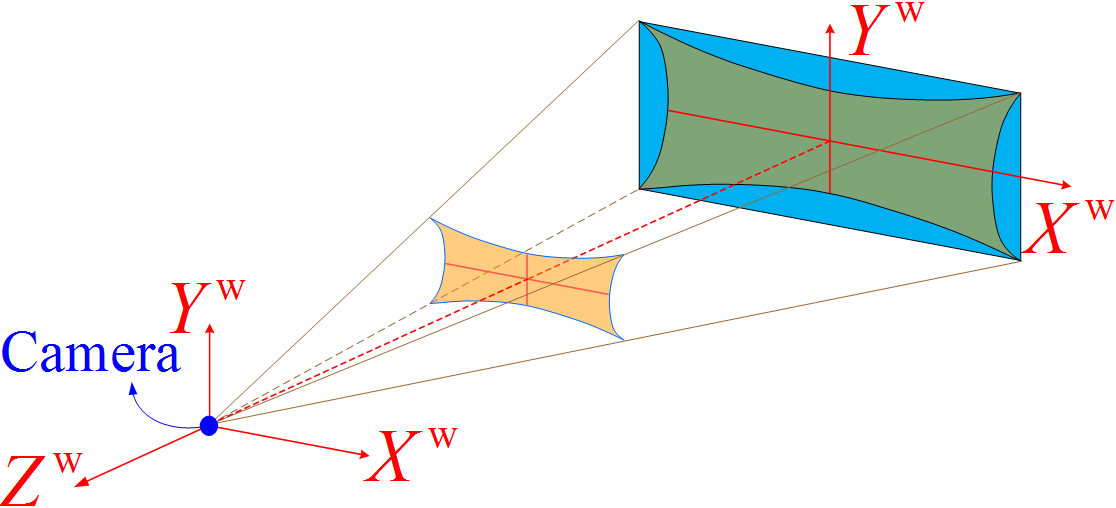
\includegraphics[width=\textwidth]{CaliPinHolCameraModel}
%\caption{Lens Distortion Removed Pinhole Camera model}
%\label{CaliPinHolCameraModel}
%\end{figure}%
%%
%
%With \(X^w\)/\(Y^w\)'s lens distortions removed, the last thing to go for is to calculate beam equations for every single pixel. It is straight forward to determine a line equation (beam equation) given two know points. The first point is the origin, and the second point could be calculated using the high order transformation matrix.
%%%%%%%%%%%%%%
%%%%%%%%%%%%%%
%%%%%%%%%%%%%%
%%%%%%%%%%%%%%
%\subsection{Extended Method Two}
%The extended method one, which is introduced above, is still not ideal. The focal point and focal length of a camera practically will change as its lens changes, so that light rays should not converge at the origin, and probably not even at one point. In order to get more accurate \gls{LUT} for a better \gls{3D} view, the second point of the beam for every single pixel should also be a datum retrieved from the camera. %
%%\\\\%
%The second method, chasing after accuracy, is to add a rail along \(Z^w\)-axis for multiple points data acquisition. Not only real points (in contrast to assuming the origin as the second point) will be used for beam equation determination, but the \(Z^w\) values could also be calibrated with external accurate data support in case \(depth\) distortion (as shown in Fig.~\ref{NIR_by_Depth_LeftSide}).
%%
%\begin{figure}[H]
%\centering
%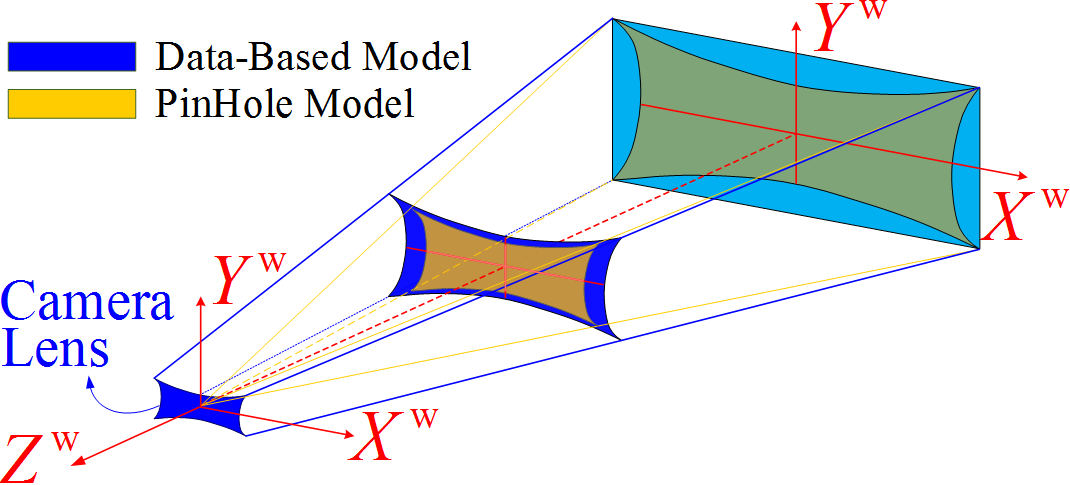
\includegraphics[width=\textwidth]{DataBasedCalibrationModel}
%\caption{Comparison: Data-Based Calibration and Pinhole Model Calibration}
%\label{DataBasedCalibrationModel}
%\end{figure}%
%%
%%
%
%Fig.~\ref{DataBasedCalibrationModel} gives the data-based model in dark blue, whereas the pinhole camera model in yellow. Due to the fact that, the lens prolongs the focal length, the light rays after lens-distortion removed will converge in front of the origin instead of at the origin. The virtual converging point, which in pinhole camera model was at the origin, is now between the origin and the view, notes as \enquote{Virtual Camera Lens}. This model is proved practically on \gls{KinectV2} in section \ref{finalDataBasedModelReconstruction} Fig.~\ref{SampleBeams_\gls{NIR}}.
%


























%\copyrightnotice
%Chapter 3
\chapter{Per-Pixel Calibration and 3D Reconstruction on GPU} % Main chapter title
\label{chapterDataBasedCalibration} 
%
%
%*.  aims to convert RGB-D camera streams in to XYZRGB on GPU.
%*. Kai showed us how to convert the pinhole camera matrix into beam equation (XYZ from P) so that it could be processed on GPU
%#. pinhole camera model
%#. GPU process, each pixel call an independent frame shader and do processing based on its screen position.
%
%*. We want to go beyond Kai:
%#. Add radial distortion correction
%#. want more generic D -> Z transformation
%#. align RGB value from a separate RGB sensor.

%Of all calibration systems, we think the best a moving XY plane, because:
%*. can take infinite number of calibration points
%*. fill up the field of view
%*. Dense D -> Z transformation

%procedures:
%1. Move the slider to the nearest position.
%a. use laser to measure distance from the slider to the pattern plane, and record the distance as $Z^W$
%b. Grab NearIR, Depth, RGB video frame
%c. Detect closest centers in NearIR + RGB frame
%d. assign XY to extracted CR of dots' centers, find high order mapping.
%e. generate dense XY for all pixels based on the high order mapping, in NearIR and RGB respectively
%
%2. move the rail to the next position, and repeat step 1.
%
%3. Unify Staggered Origin (make sure the point XY=0 is at same dot)
%4. determine per-pixel mapping coefficients of D -> Z, Z -> XY, and generate row by column by 6 look-up table
%5. RGB values alignment based on pinhole camera model.
%
%
RGBD cameras are famous for its 3D reconstruction application. In this chapter, we will show how to reconstruct 3D image naturally on GPU in camera space based on raw data without calibration. Considering the deformation of raw data resulted from lens distortions and \emph{depth distortion}, we propose a per-pixel calibration method based on a rail calibration system. Instead of using a pinhole-camera model, a two-dimensional high-order polynomial mapping model is determined and employed for lens distortions removal. Corresponding data collection procedures and look-up table based undistorted real-time world space 3D reconstruction on GPU are discussed in detail. Color values alignment is also discussed at last.
%
\section{\(RGBD\) to \(X^CY^CZ^CRGB\)}
\label{sectionCameraSpaceReconstruction}
As described in chapter \ref{chapterIntroduction}, there are applications like SLAM and KinectFusion that require \(D\) to be converted into \(X^CY^CZ^C\) coordinates on a per-pixel basis. From Chapter \ref{chapterTraditionalCalibration}, we know that the depth sensor measures \(Z^C\), and a pinhole camera model (more specifically the intrinsic matrix) in homogeneous coordinates offers the relationship between \(Z^C\) and \(X^C/Y^C\) respectively. In this section, we will introduce how to generate the camera space 3D coordinates without calibration, and draw a camera space 3D reconstruction on GPU using a KinectV2 camera.
\\\indent
%
\begin{figure}[!b]
\centering
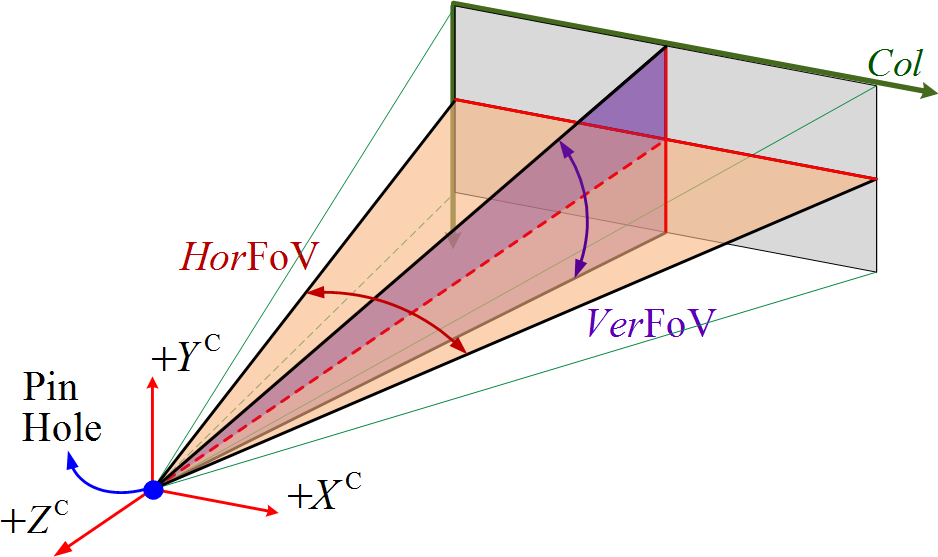
\includegraphics[width=0.7\textwidth]{VHfieldOfView}
\caption{Field of View in Pinhole-Camera Model}
\label{VHfieldOfView}
\end{figure}%
%
The KinectV2 depth sensor measures \(Z^C\) in millimeter and supports its positive data in unsigned-short data-type. Those data will be automatically converted into single-floating type with its range from 0.0f to +1.0f when uploaded onto GPU. Considering that in practice \(D\)s from KinectV2 are always positive whereas \(Z^C\)s should be always negative, we will add a negative sign in the un-scaling step to recover the \(Z^C\) in metric on GPU:
\begin{equation}
Z^C[m, n] = - \beta D[m, n] \, ,
\label{unscalingZc}
\end{equation}%
\noindent
where \(\beta\) constantly equals to 65535.0 (range of unsigned short in single-floating) for all pixels. Besides the depth stream, KinectV2 supports both of the horizontal and vertical field of view (FoV) that can help generate per-pixel \(X^C\) and \(Y^C\), which share the same credits with the intrinsic parameters in a pinhole camera model. Figure~\ref{VHfieldOfView} shows an intuitive view of the horizontal and vertical FoVs in a pinhole camera model, based on which we can derive the \(X^C\) and \(Y^C\) values given a random \(Z^C\) value on the per-pixels basis. Assuming the depth sensor, with its size numDepthRows by numDepthCols, is observing right perpendicularly to a wall where all pixels share the same \(|Z^C_0|\) from the sensor to the wall. Talking about the horizontal FoV only, it is easy to get the range of the camera space FoV along 
\(X^C\)-axis from \(-|X^C_{\text{Max}}|\) to \(|X^C_{\text{Max}}|\), as shown in Fig.~\ref{horizontalFoVtoColumns}. %
\begin{figure}[!t]
\centering
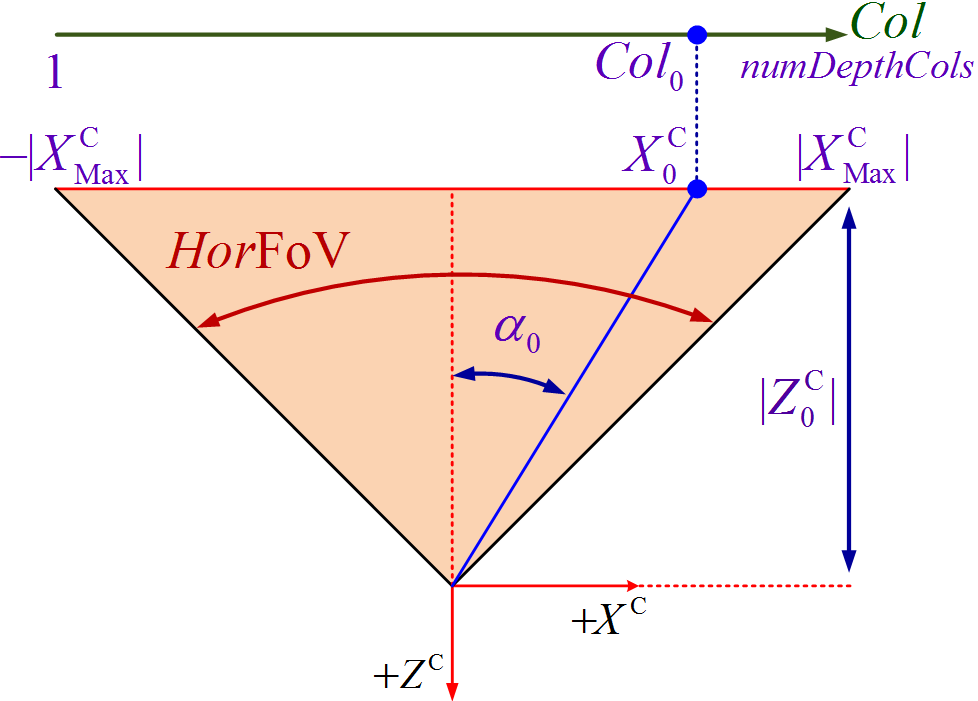
\includegraphics[width=0.6\textwidth]{horizontalFoVtoColumns}
\caption{map \(Col\) to \(X^C\) via horizontal FoV}
\label{horizontalFoVtoColumns}
\end{figure}%
%
The horizontal range value \(|X^C_{\text{Max}}|\) depends on \(|Z^C_0|\) and the horizontal FoV, given by:
%
\begin{equation}
|X^C_{\text{Max}}| = |Z^C_0| \cdot tan(horFov / 2) 
\label{cameraXMaxfromZ}
\end{equation}%
\noindent
where the pixel observing on \(X^C = |X^C_{\text{Max}}|\) has its column address of numDepthCols. Similarly, given a random pixel of column address \(Col_0\), its horizontal view \(X^C_0\) could be expressed based on its own horizontal view angle \(\alpha_0\).
%
\begin{equation}
|X^C_{0}| = |Z^C_0| \cdot tan(\alpha_0)
\label{alphaZeroHorFOV}
\end{equation}%
\noindent
To combine eqn.~(\ref{cameraXMaxfromZ}) and eqn.~(\ref{alphaZeroHorFOV}), we get
%
\begin{equation}
\frac{X^C_0}{|X^C_{\text{Max}}|} = \frac{tan(\alpha_0)}{tan(horFov / 2)} = \frac{Col_0}{numDepthCols} - 0.5 \, ,
\label{alphaZeroHorFOV}
\end{equation}%
\noindent
which shows how to get the per-pixel \(X^C_0\) from \(|X^C_{\text{Max}}|\) based on its column address, while \(|X^C_{\text{Max}}|\) depends on the depth sensor's horizontal filed of view. It is intuitively better to change eqn.~(\ref{alphaZeroHorFOV}) a little by substituting \(|X^C_{\text{Max}}|\) with eqn.~(\ref{cameraXMaxfromZ}) such that we can get eqn.~(\ref{proportionalEqnFromZtoX}), a proportional per-pixel mapping based on the column addresses from \(Z^C\) to \(X^C\).
%
\begin{equation}
X^C[m, n] = tan(horFov / 2) \cdot (\frac{n}{numDepthCols} - 0.5) \cdot |Z^C[m, n]|\, ,
\label{proportionalEqnFromZtoX}
\end{equation}%
\noindent
where [\(m,n\)] is the discrete space \(row\) and \(column\) coordinate of each pixel in the depth sensor. Similarly, we can also get the proportional per-pixel mapping from \(Z^C\) to \(Y^C\), based on the vertical FoV and row addresses.
%
\begin{equation}
Y^C[m, n] = tan(verFov / 2) \cdot (\frac{m}{numDepthRows} - 0.5) \cdot |Z^C[m, n]|
\label{proportionalEqnFromZtoY}
\end{equation}%
\noindent
Note that, \(horFov\) and \(verFov\) are constant during image processing, such that the mapping functions from per-pixel \(Z^C\) to per-pixel \(X^C/Y^C\) totally depend on a pixel's address [\(m, n\)]. Therefore eqn.~(\ref{proportionalEqnFromZtoX}) and eqn.~(\ref{proportionalEqnFromZtoY}) could be expressed as 
%
\begin{equation}
\begin{aligned}
X^C[m, n] &= a[m, n] \cdot |Z^C[m, n]|
\\%
Y^C[m, n] &= b[m, n] \cdot |Z^C[m, n]| 
\end{aligned}
\label{proportionalBeamEqn}
\end{equation}%
\noindent
where
%
\begin{equation}
\begin{aligned}
a[m, n] &= tan(horFov / 2) \cdot (\frac{n}{numDepthCols} - 0.5)
\\%
b[m, n] &= tan(verFov / 2) \cdot (\frac{m}{numDepthRows} - 0.5) \, \, .
\end{aligned}
\label{parametersABofProportional}
\end{equation}%
\\\indent
%
\begin{figure}[!t]
\centering

\includegraphics[width=0.8\textwidth]{cameraSpaceDiagram}
\caption{Diagram for Camera Space 3D Reconstruction without calibration}
\label{cameraSpaceDiagram}
\end{figure}%
%
Now that we have the per-pixel mapping from \(Z^C\) to \(X^CY^C\), it is time to draw the camera space 3D image on GPU. Figure~\ref{cameraSpaceDiagram} shows the streams flow diagram. We will retrieve \(Depth\) streams from the KinectV2 camera, save them into corresponding buffers on CPU and upload the the streams onto GPU as textures. Then the per-pixel's camera space 3D coordinates \(X^CY^CZ^C\) will be generated during its fragment-shader processing from depth texture based on eqn.~(\ref{proportionalBeamEqn}). The fragment shader is programmed as below.
\\%
{\ttfamily
\textbf{\textcolor[rgb]{0.5019608,0.5019608,0.0}{\ \ \ uniform }}\textcolor[rgb]{0.7529412,0.7529412,0.7529412}{
 }\textcolor[rgb]{0.5019608,0.5019608,0.0}{sampler2D }\textcolor[rgb]{0.7529412,0.7529412,0.7529412}{
}qt\_depthTexture;\textcolor[rgb]{0.7529412,0.7529412,0.7529412}{
\ \ }}

{\ttfamily
\textbf{\textcolor[rgb]{0.5019608,0.5019608,0.0}{uniform }}\textcolor[rgb]{0.7529412,0.7529412,0.7529412}{
 }\textcolor[rgb]{0.5019608,0.5019608,0.0}{sampler2D }\textcolor[rgb]{0.7529412,0.7529412,0.7529412}{
}qt\_spherTexture;\textcolor[rgb]{0.7529412,0.7529412,0.7529412}{ \ }}


\bigskip

{\ttfamily
\textbf{\textcolor[rgb]{0.5019608,0.5019608,0.0}{layout}}(\textbf{\textcolor[rgb]{0.5019608,0.5019608,0.0}{location } }\textcolor[rgb]{0.7529412,0.7529412,0.7529412}{
}=\textcolor[rgb]{0.7529412,0.7529412,0.7529412}{
}0,\textcolor[rgb]{0.7529412,0.7529412,0.7529412}{
}\textbf{\textcolor[rgb]{0.5019608,0.5019608,0.0}{index } }\textcolor[rgb]{0.7529412,0.7529412,0.7529412}{
}=\textcolor[rgb]{0.7529412,0.7529412,0.7529412}{
}0)\textcolor[rgb]{0.7529412,0.7529412,0.7529412}{
}\textbf{\textcolor[rgb]{0.5019608,0.5019608,0.0}{out } }\textcolor[rgb]{0.7529412,0.7529412,0.7529412}{
 }\textcolor[rgb]{0.5019608,0.5019608,0.0}{vec4 }\textcolor[rgb]{0.7529412,0.7529412,0.7529412}{
}qt\_fragColor;}

{\ttfamily
\textcolor[rgb]{0.5019608,0.5019608,0.0}{void }\textcolor[rgb]{0.7529412,0.7529412,0.7529412}{
}main()}

{\ttfamily
\{}

{\ttfamily
\textcolor[rgb]{0.7529412,0.7529412,0.7529412}{\ \ \ \  }\textcolor[rgb]{0.5019608,0.5019608,0.0}{ivec2 }\textcolor[rgb]{0.7529412,0.7529412,0.7529412}{
}textureCoordinate\textcolor[rgb]{0.7529412,0.7529412,0.7529412}{
}=\textcolor[rgb]{0.7529412,0.7529412,0.7529412}{
 }\textcolor[rgb]{0.5019608,0.5019608,0.0}{ivec2}(
 \textcolor[rgb]{0.5019608,0.0,0.5019608}{gl\_FragCoord}.x, \textcolor[rgb]{0.7529412,0.7529412,0.7529412}{
 }\textcolor[rgb]{0.5019608,0.0,0.5019608}{gl\_FragCoord}.y);}

\bigskip

{\ttfamily
\textcolor[rgb]{0.7529412,0.7529412,0.7529412}{\ \ \ \ }\textcolor[rgb]{0.5019608,0.5019608,0.0}{float}\textcolor[rgb]{0.7529412,0.7529412,0.7529412}{
}z\textcolor[rgb]{0.7529412,0.7529412,0.7529412}{
} = \textcolor[rgb]{0.7529412,0.7529412,0.7529412}{
}\textbf{\textcolor[rgb]{0.5019608,0.5019608,0.0}{texelFetch}}(qt\_depthTexture,\textcolor[rgb]{0.7529412,0.7529412,0.7529412}{
}textureCoordinate,\textcolor[rgb]{0.7529412,0.7529412,0.7529412}{
}\textcolor[rgb]{0.0,0.0,0.5019608}{0}).r
*\textcolor[rgb]{0.7529412,0.7529412,0.7529412}{
}\textcolor[rgb]{0.0,0.0,0.5019608}{65535.0};}

{\ttfamily
\textcolor[rgb]{0.7529412,0.7529412,0.7529412}{\ \ \ \ }\textcolor[rgb]{0.5019608,0.5019608,0.0}{vec4}\textcolor[rgb]{0.7529412,0.7529412,0.7529412}{
\ }a\textcolor[rgb]{0.7529412,0.7529412,0.7529412}{
} = \textcolor[rgb]{0.7529412,0.7529412,0.7529412}{
}\textbf{\textcolor[rgb]{0.5019608,0.5019608,0.0}{texelFetch}}(qt\_spherTexture,\textcolor[rgb]{0.7529412,0.7529412,0.7529412}{
}textureCoordinate,\textcolor[rgb]{0.7529412,0.7529412,0.7529412}{
}\textcolor[rgb]{0.0,0.0,0.5019608}{0});}


\bigskip

{\ttfamily
\textcolor[rgb]{0.7529412,0.7529412,0.7529412}{\ \ \ \ }qt\_fragColor.x\textcolor[rgb]{0.7529412,0.7529412,0.7529412}{
} = \textcolor[rgb]{0.7529412,0.7529412,0.7529412}{
}{}-z\textcolor[rgb]{0.7529412,0.7529412,0.7529412}{
}*\textcolor[rgb]{0.7529412,0.7529412,0.7529412}{ }a.r;}

{\ttfamily
\textcolor[rgb]{0.7529412,0.7529412,0.7529412}{\ \ \ \ }qt\_fragColor.y\textcolor[rgb]{0.7529412,0.7529412,0.7529412}{
} = \textcolor[rgb]{0.7529412,0.7529412,0.7529412}{
}{}-z\textcolor[rgb]{0.7529412,0.7529412,0.7529412}{
}*\textcolor[rgb]{0.7529412,0.7529412,0.7529412}{ }a.g;}

{\ttfamily
\textcolor[rgb]{0.7529412,0.7529412,0.7529412}{\ \ \ \ }qt\_fragColor.z\textcolor[rgb]{0.7529412,0.7529412,0.7529412}{
} = \textcolor[rgb]{0.7529412,0.7529412,0.7529412}{ }{}-z;}

{\ttfamily
\}}

%
The uniform \emph{qt\_spherTexture} is a \(Z^C\) to \(X^C/Y^C\) proportional mapping texture, which contains the per-pixel parameters \(a/b\) based on eqn.~(\ref{parametersABofProportional}). Note that we add three negative signs in front of \(X^CY^CZ^C\) respectively to account for the pinhole-imaging. %
%
\begin{figure}[t]
\centering
\subfloat[Front View][Front View]{
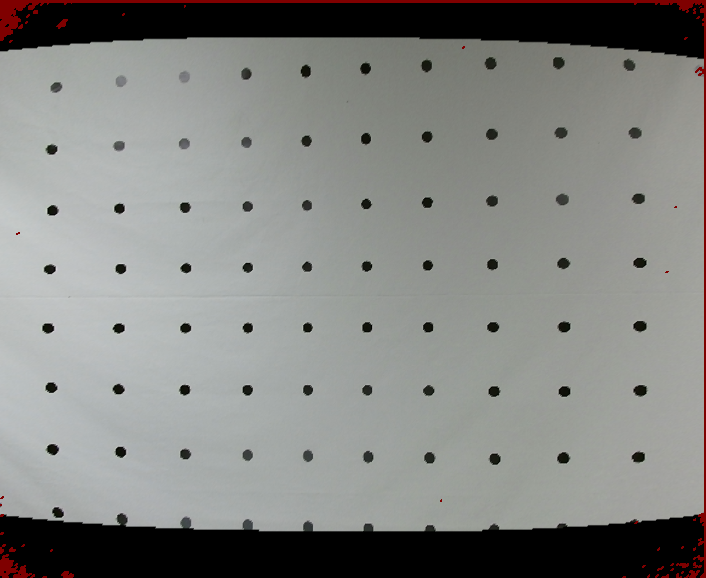
\includegraphics[height=0.42\textwidth]{distortedRGB}
\label{distortedRGB}}
\subfloat[Left View][Left View]{

\includegraphics[height=0.42\textwidth , width = 0.4\textwidth]{distortedSideViewRGB}
\label{distortedSideViewRGB}}
%\qquad
\caption{Colored Camera Space 3D Reconstruction}
\label{reconstructionInCameraSpace}
\end{figure}%
%
The whole parallel image processing above shows a natural 3D reconstruction on GPU. Figure~\ref{reconstructionInCameraSpace} shows the view of camera space 3D reconstruction when observing uniform grid dots pattern on the flat wall. We can tell from the image that, this reconstruction is totally based on raw data, without calibration at all. Not only the \(X^CY^C\) plane is apparently deformed (lens distortions) in the front view, but the \(Z^C\) is also not as flat as it should be, which we will call it \emph{depth distortion} since now. The \emph{depth distortion} comes from the imperfect depth resolutions among pixels, \textit{i.e.}, \(Z^C_{[row, col]} - Depth_{[row, col]} \neq E_{\text{Constant}}\), which lead to bumps and hollows in the camera space reconstruction when observing a flat wall. Therefore, a per-pixel calibration is necessary for an undistorted 3D image.

%%%%%%%%%%%%%%%%%%%%%%%%%%%%%%%%%%%%%%%%%%%%%%%%%%%%%%%%%%%%%%%%%%%%%%%%%%%%%%%%%%%%%%%%%%%%%%%%%%%%%%%%%%%%%%%%%%%%%%%%%%%%%%%%%%%%%%%%%%%%%%%%%%%%%%%%%%%%%%%%%%%%%%%%%%%%%%%%%%%%%%%%%%%%%%%%%%%%%%%%%%%%%%%%%%%%%%%%%%%%%%%%%%%%%%%%%%%%%%%%%%%%%%%%%%%%%%%%%%%%%%%%%%%%%%
\section{Rail Calibration System}
\label{sectionRailCalibrationSystem}
Talking about camera calibration, the pinhole camera matrix \(M\) will come up in most people's mind. As discussed in Chapter~\ref{chapterTraditionalCalibration}, the pinhole-camera matrix \(M\) consists of an intrinsic matrix \(K\) and an extrinsic matrix \([R_{3*3}, T_{3*1}]\). The camera space 3D reconstruction method we discussed in section~\ref{sectionCameraSpaceReconstruction} utilizes horizontal and vertical field of view (FoV)s, which works in the same way with the intrinsic matrix \(K\)'s principle. However, a camera's calibration needs external help from world space objects, which means neither of the FoVs nor intrinsic matrix \(K\) alone is able to do calibration,  and extrinsic parameters that can link to world space are necessary in calibration. 
\\\indent
Kai \cite{Kai10} did a good job on structured light 3D scanner parallel calibration on GPU, and derived the per-pixel beam equation~(\ref{kaiBeamEquationCh3}) directly from a pinhole camera matrix \(M\), which offers the possibility of natural 3D reconstruction on GPU similar to eqn.~(\ref{proportionalBeamEqn}).
%
\begin{equation}
\begin{aligned}
X^W[m,\,  n] = a[m, n]Z^W[m,\,  n]+b[m, n]
\\%
Y^W[m,\,  n] = c[m, n]Z^W[m,\,  n]+d[m, n]
\end{aligned}
\label{kaiBeamEquationCh3}
\end{equation}%
\noindent
where [\(m,n\)] is the discrete space \(row\) and \(column\) coordinate of each pixel in a M by N sensor. This per-pixel beam equation shows per-pixel linear mappings from \(Z^W\) to \(X^W/Y^W\), and the per-pixel \(Z^W\) can be mapped from features of structured light. It is not specially proportional like eqn.~(\ref{proportionalBeamEqn}), because it contains space translation infos from camera space to world space. Although it is in world space now and the intrinsic parameters are able to be determined, however, lens distortions are still not able to be handled. To make it ideal, we need to not only remove the lens distortions and \emph{depth distortion}, but also realize the 3D reconstruction on GPU in a natural method similar to eqn.~(\ref{kaiBeamEquationCh3}).
\\\indent
%
In this section, we will find a best-fit calibration system for a KinectV2 camera's natural calibration and reconstruction, which is able the handle both of lens distortion and \emph{depth distortion}. %
%The KinectV2 camera has one depth sensor and one RGB sensor. The RGB sensor offers RGB streams, whose color infos will be aligned to pixels according to their corresponding world space coordinates after the 3D reconstruction. The depth sensor offers NearIR and Depth streams, both of which share the same size ($row$ and $column$) and lens distortions of the depth sensor, and can both be utilized for lens distortion correction. We will use the Depth stream to recover world space 3D coordinates $X^WY^WZ^W$ for reconstruction, during which the NearIR stream will be used for lens distortion correction. 
%\\\indent
To easily show 3D reconstruction in a parallel way on the GPU, we would like our calibration system to be able to offer a per-pixel mapping from \(D\) to \(Z^W\), which then could be used to map to \(X^W/Y^W\) using eqn.~(\ref{kaiBeamEquationCh3}). In this way, the \emph{depth distortion} could also be corrected during the per-pixel \(D\) to \(Z^W\) mapping.
%
\begin{figure}[t]
\centering
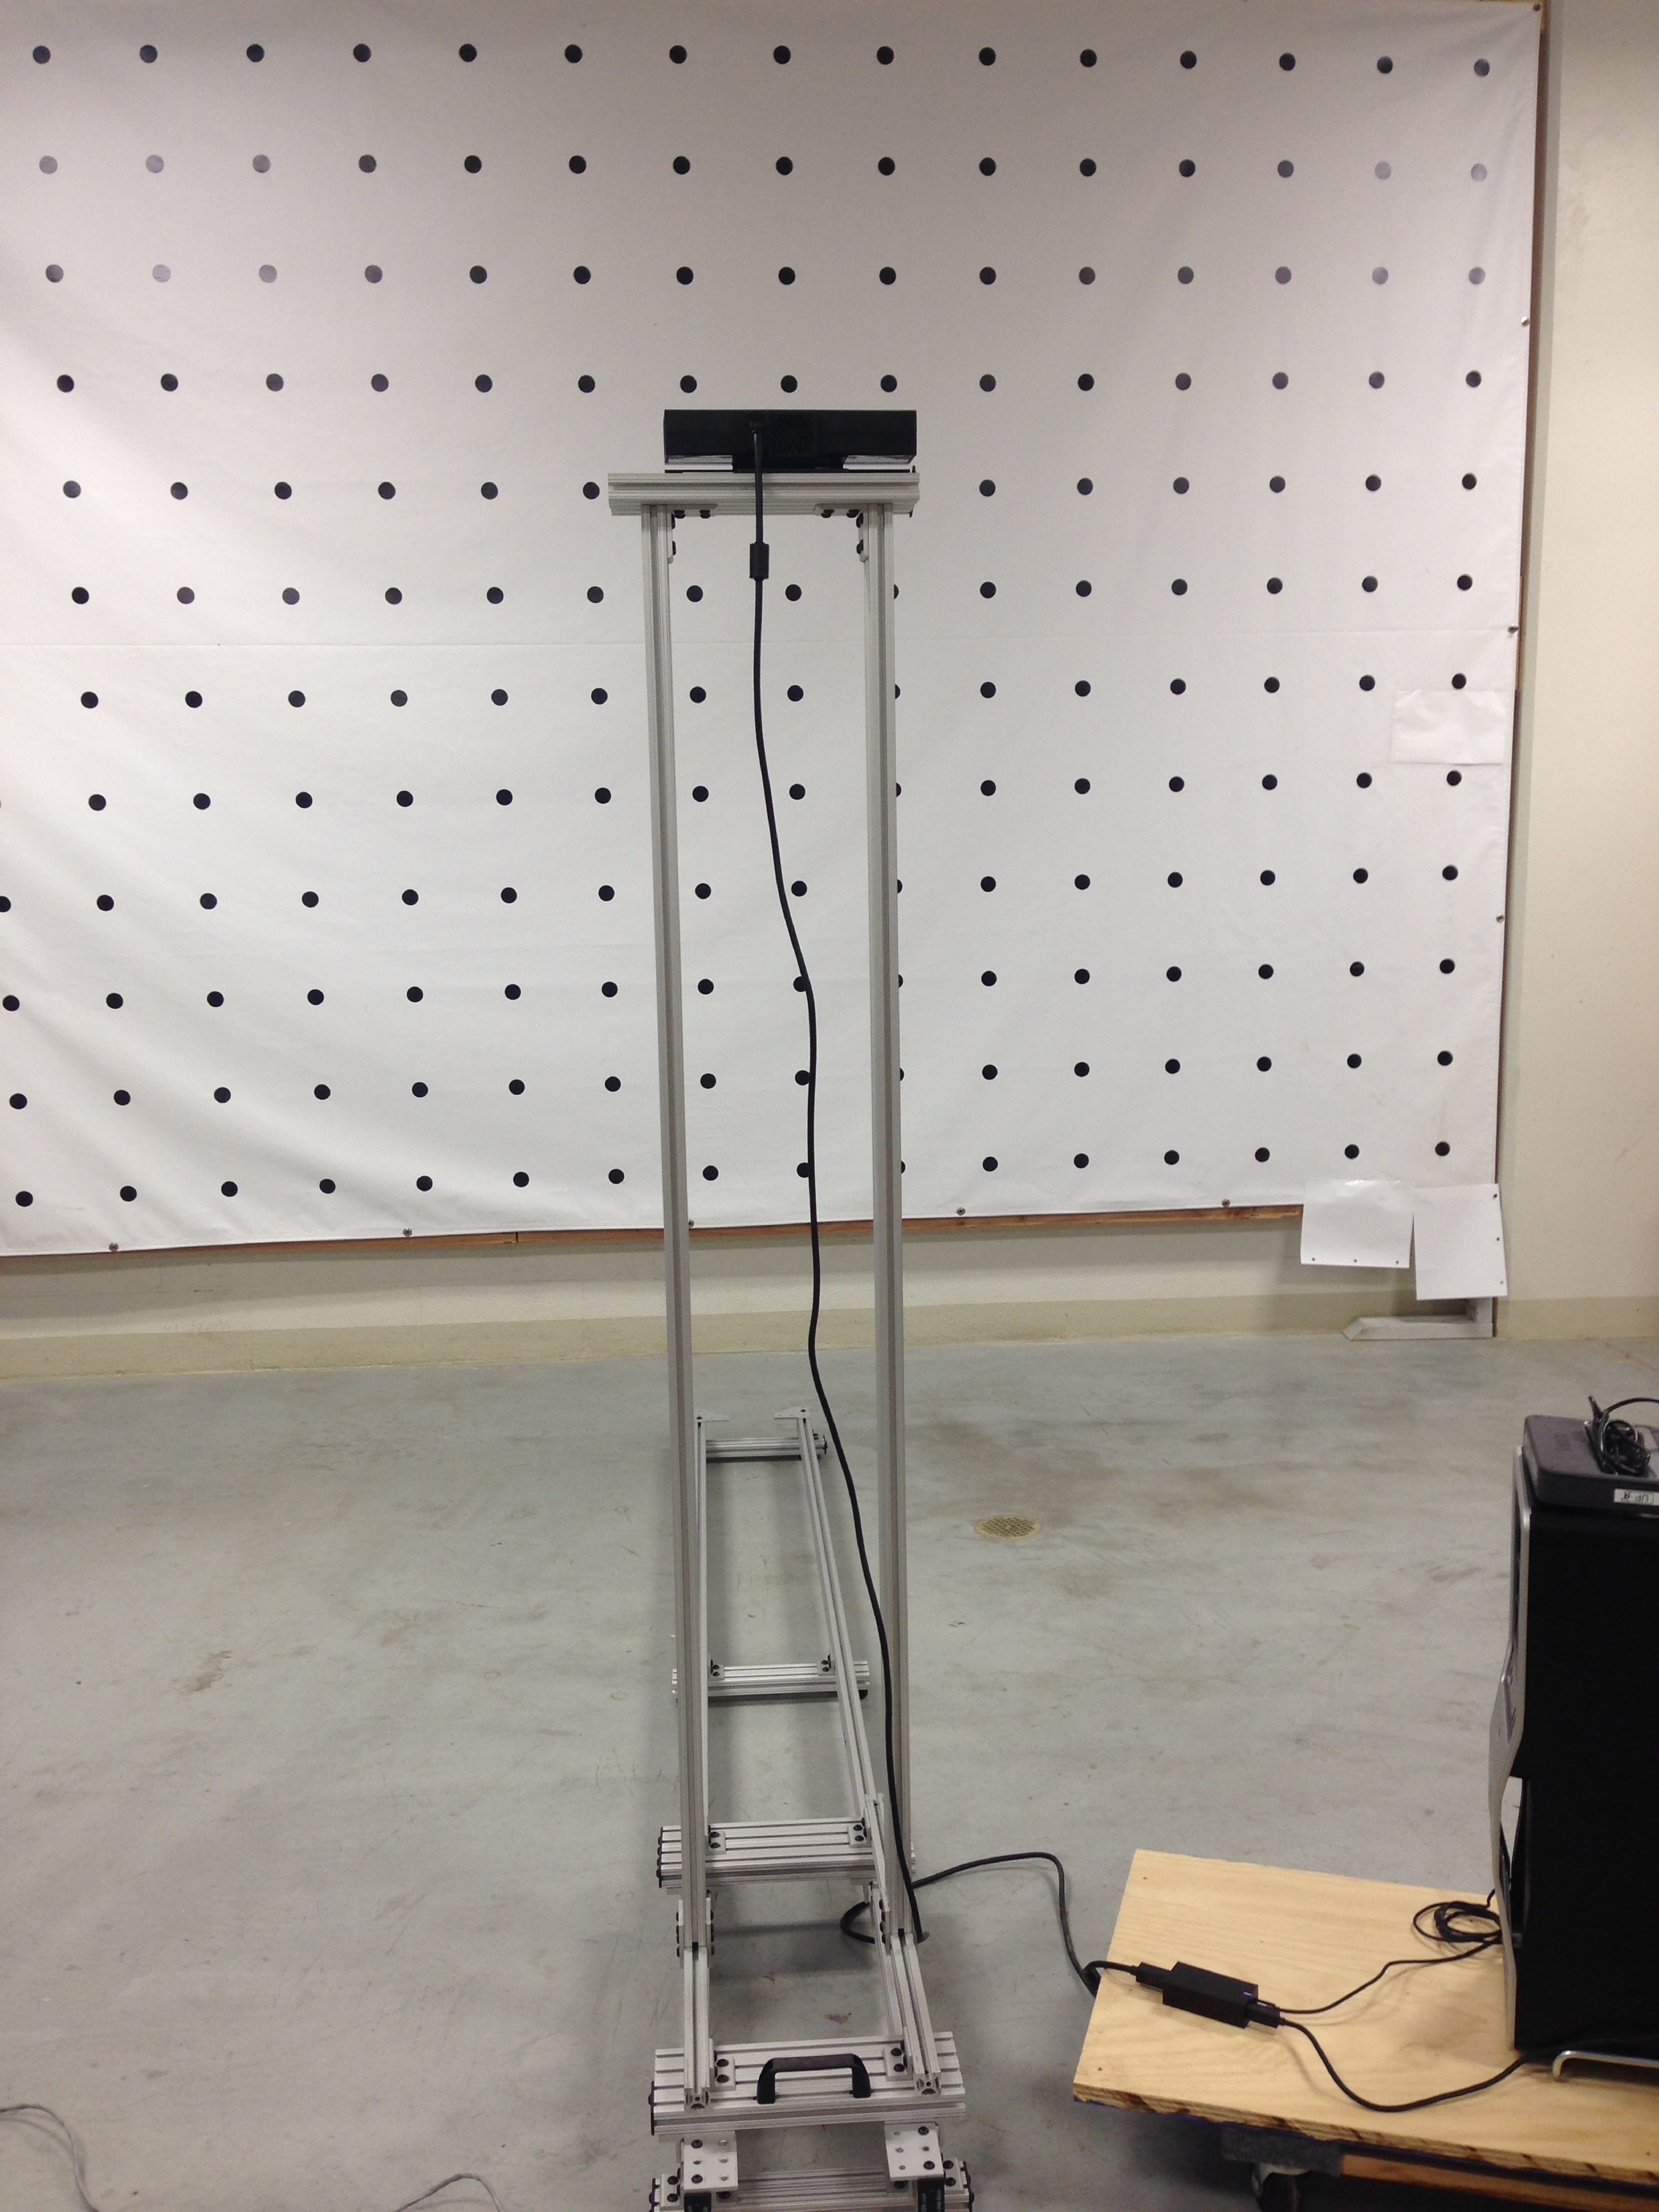
\includegraphics[width=0.55\textwidth]{trackingModuleOnKinectV2CalibrationSystem}
\caption{KinectV2 Calibration System}
\label{trackingModuleOnKinectV2CalibrationSystemCh3}
\end{figure}%
%
Of all different kinds of calibration systems, a camera on rail system with a planar pattern on wall is finally decided, which offers a moving plane with respect to the camera when the camera moves along the rail. As Fig.~\ref{trackingModuleOnKinectV2CalibrationSystemCh3} shows, a canvas on which printed an uniform grid dots pattern is hung on the wall, and the rail is required to be perpendicular to the wall. The RGB-D camera waiting to calibrate is mounted on the slider. Note that, in this calibration system, the only unit that needs to be perpendicular to the wall is the rail, whereas the RGB-D camera has no need to require its observation orientation. Because the per-pixel calibration requires only accurate world space coordinates which will be decided by the rail and the wall, whereas the camera's space is not considered at all. We will assign the pattern plane as the \(X^WY^W\) plane in world space, and the rail to be along with (not exactly on) \(Z^W\)-axis. The world coordinate is static with the camera on the slider. %
%
\begin{figure}[!t]
\centering
%calibrated \(X^{W}\)/\(Y^{W}\) and \(Z^{W}\)
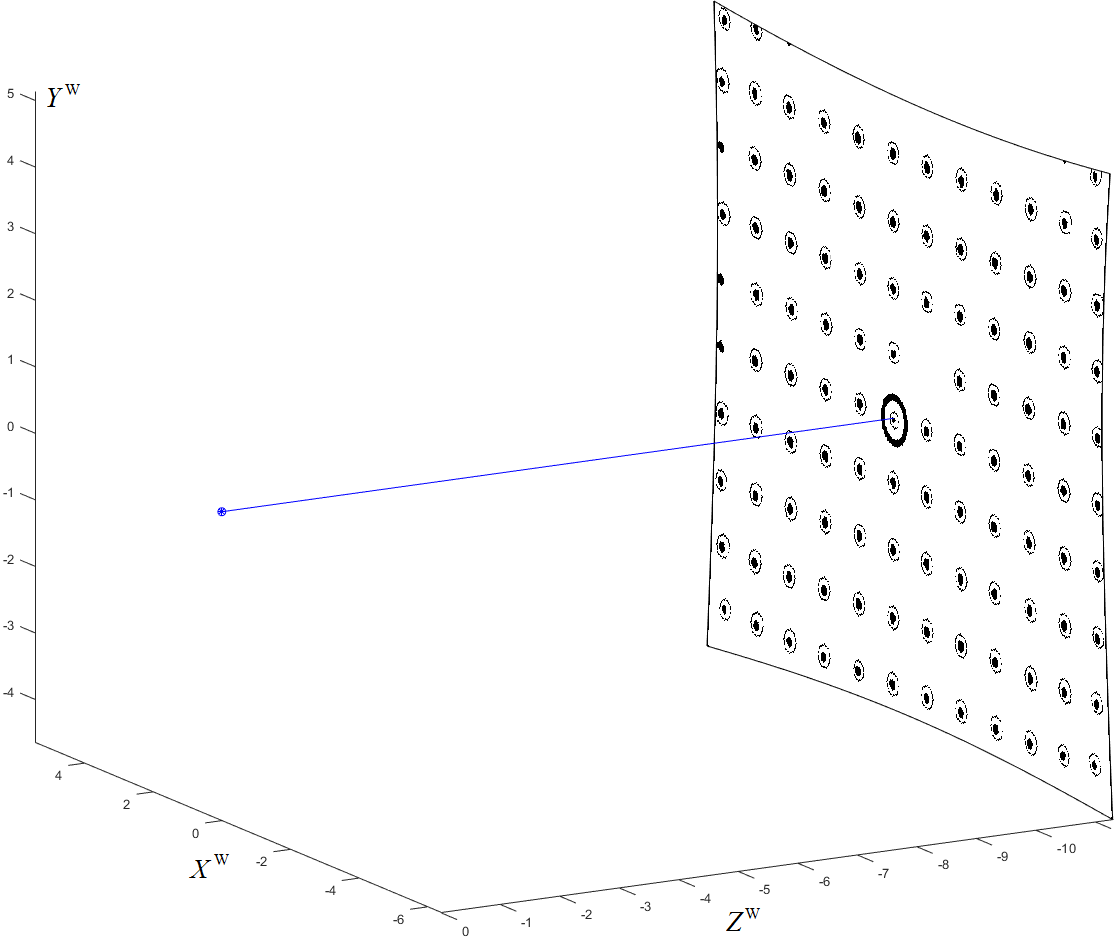
\includegraphics[width=0.7\textwidth, height= 0.5\textwidth]{OneFrameXYZ_Calibrated}
\caption{NearIR \(X^{W}Y^{W}Z^{W}\) 3D Reconstruction}
\label{OneFrameXYZ_Calibrated}
\end{figure}%
%
\\\indent
Figure~\ref{OneFrameXYZ_Calibrated} shows one frame of NearIR \(X^WY^WZ^W\) 3D reconstruction, which can help a lot explaining how the world space origin is assigned. Inside the figure, both of the origin and \(Z\)-axis are high-lighted in blue, and the origin of world space is on the left end of the blue line. On the pattern plane with dot-clusters marked in circles, we can see one dot-cluster is high-lighted inside a thick circle, and its center point is where \(X^W/Y^W = 0\). The dot-cluster which will be sitting on the \(Z^W\)-axis is the one whose center point is closest to the center pixel of the sensor. All pixels in this frame share the exact same \(Z^W\), which is also why we require the rail to be perpendicular to the pattern. And the value of \(Z^W\) is measured by a laser distance measurer that static with the camera. The final origin of the world space will be decided by both of the camera's observing orientation and the laser distance measurer's position. This kind of world coordinate assignment is totally for simplifying image processing during calibration.  Practically, we do not even care where exactly the origin is, as long as the rail is perpendicular to the pattern and the distance measurer is static with the camera.
\\\indent
With this rail calibration system, infinite number of frames with infinite number of calibration points could be utilized for training a calibration model. Besides, as the slider moves along the rail, the amount and distribution of the grid dots captured by the camera will change, which means a dynamic pattern for calibration instead of static. With more and more dots walking into the camera's field of view under a certain rhythm as the slider moves further from the pattern plane, the dots (which will be extracted as calibration points) are able to cover all pixels of a sensor. What's more, a moving-plane system (multiple frames calibration instead of one frame calibration) makes it possible to do dense \(D\) to \(Z^W\) mapping, which will handle \emph{depth distortion}.


\section{Data Collection}
\label{perpixelDataCollection}
%
With the calibration system built up and world coordinate assigned, we are now ready to calibrate. \(Z^{W}\) values for all pixels of every frame will be supported from external laser distance measurer. To simplify potential calculation during image processing, we assign the world coordinate \emph{Unit One} based on the uniform grid dots patter, to be same with the side of pattern's unit-square. Concretely, the distance between every two adjacent dots' centers in real-world is 228mm. Therefore, \(Z^{W}\) = -\(Z\)(mm) / 228(mm), where \(Z\) is the vertical distance to the pattern plane in reality measured by the laser distance measurer. Note that, \(Z^{W}\) values are always negative, based on the assignment of Cartesian world coordinate. The outline of calibration procedures is listed below.
%
\begin{enumerate}
   	\item Mount both of the camera and laser distance measurer onto the slider.
   	\item Move the slider to the nearest position to the pattern plane.
   	\item Record one frame of RGB data with one frame of NearIR data at this position.
   	\label{repeatMovingSlider}
   	\begin{enumerate}
     		\item measure \(|Z^W|\) using the laser distance measurer.
     		\item grab RGB, NearIR and Depth streams from KinectV2 camera.
     		\item extract center points (\(R/C\)) of dot-clusters from RGB and NearIR streams respectively.
     		\item assign \(X^W/Y^W\) values to the extracted points, RGB and NearIR respectively.
     		\item train and determine the best-fit high order polynomial model that map from \(RC\) to \(X^W/Y^W\), RGB and NearIR respectively.
     		\item generate dense \(X^W/Y^W\) for all pixels using the model, for NearIR and RGB streams respectively.
     		\item save 2 frames of RGB and NearIR all pixels' data respectively: \(X^WY^WZ^WRGBD\) for RGB stream, and \(X^WY^WZ^WID\) for NearIR stream, where the channel \(I\) in NearIR frame denotes \emph{Intensity}.
   	\end{enumerate}
	\item Move the slider to the next position, and repeat step~\ref{repeatMovingSlider}.
%	\item Check all \(X^W/Y^W\) values of all frames, unify the staggered origin by adding or subtracting a corresponding integer (make sure the point \(X^WY^W = 0\) is at the same dot-cluster for all frames).
%	\item Determine the per-pixel mapping from \(D\) to \(Z^W\) and from \(Z^W\) to \(X^W/Y^W\) for all pixels using the NearIR frames of data, and generate a \(row\)-by-\(column\)-by-6 look-up table.
%	\item Determine a pinhole-camera matrix that can map \(X^W/Y^W/Z^W\) to \(R/C\) using RGB frames of data (for the RGB values' alignment to pixels after 3D reconstruction).
\end{enumerate}
%
Concretely, we will record RGB and NearIR frames every 25mm at a time. During every time, \(|Z^W|\) will be measured by the laser measurer and manually input into the shader at the very beginning of streams recording. After RGB, NearIR and Depth streams have been retrieved from KinectV2, we will utilize digital image processing (DIP) techniques to extract the center points' image addresses (\(R/C\)) of dot-clusters, and then determine a high-order polynomial model to build a mapping from \(RC\) to \(X^W/Y^W\) for dense world coordinates generation.

\subsection{DIP Techniques on (\(R,\, C\)) Extraction}
\label{sectionDIPTechniques}
%  add noises analysis
\indent
A robust DIP process on the extraction the points' addresses (\(R,\, C\))s determines the accuracy of calibration. In this project, the extraction steps consist of gray-scaling, histogram equalization, adaptive thresholding and a little trick on black pixels counting. OpenGL is selected as the GPU image processing language. The default data type of steams saved on GPU during processing is single-floating, with a range from 0 (balck) to 1 (white). 
\\\indent
Gray-scaling is done to unify processing steps of both RGB and NearIR steams. For NearIR steam, its data contains only color gray and data will be saved on GPU as single-floating automatically. Whereas for RGB steam, a conversion from RGB to gray value is needed. Typically, there are three converting methods: lightness, average, and luminosity. The luminosity method is finally chosen as a human-friendly way for gray-scaling, give by
%
\begin{equation}
Intensity_{\text{\_gray}} =  0.21 Red\,  + \, 0.72 Green \, + \, 0.07 Blue  \, \, ,
\label{luminosityGrayScaling}
\end{equation}%
which uses a weighted average value to account for human perception.
\\\indent%
The pixel intensity values are automatically converted into single-floating type with its range from 0.0f to 1.0f, where \enquote{0.0f} means 100\% black and \enquote{1.0f}  means 100\% white. In practice, NearIR steam image is always very dark, as shown in Fig.~\ref{Raw_Single_NIR} (with their intensity values every close to zero).  In order to enhance the contrast of NearIR image for a better binarizing, histogram equalization technique is utilized to maximize the range of valid pixel intensity distributions. Same process is also compatible on the RGB stream.
%
 \begin{figure}[t]
\hspace*{-0.5cm}
\centering
\subfloat[Raw NearIR][Raw]{

\includegraphics[width=0.5\textwidth]{Raw_Single_NIR}
\label{Raw_Single_NIR}}
\subfloat[Histogram Equalized NearIR][Histogram Equalized]{
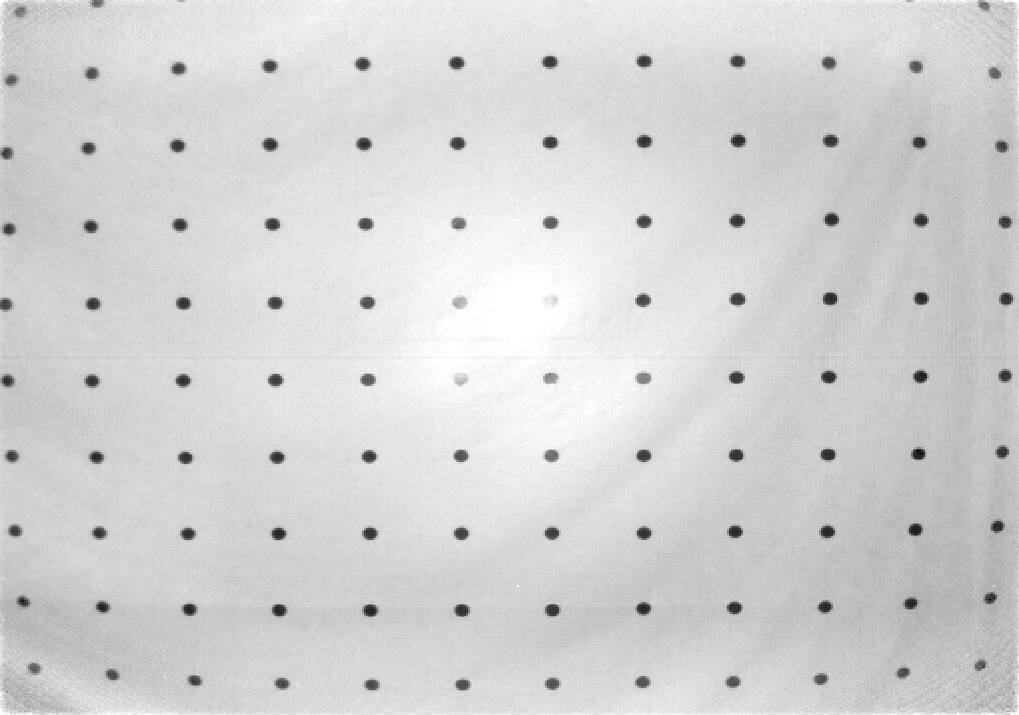
\includegraphics[width = 0.5\textwidth]{NIR_After_HistogramEqualization}
\label{NIR_After_HistogramEqualization}}
%\qquad
\caption{NearIR Streams before / after Histogram Equalization}
\label{Histogram_Equalization}
\end{figure}%
%
Commonly, Probability Mass Function (PMF) and Cumulative Distributive Function (CDF) will be calculated to determine the minimum valid intensity value (\(floor\)) and maximum valid value (\(ceiling\)) for rescaling, whereas tricks could be used by taking advantage of the GPU drawing properties.%
\\\indent%
PMF means the frequency of every valid intensity value for all of the pixels in an image. The calculation of PMF on GPU will be very similar to points' drawing process, both of which are on a per-pixel basis. Dividing all of the pixels in terms of their intensity values into \(N\) levels, every pixel belongs to one level of them, which is called gray level. With a proper selection of \(N\) to make sure a good accuracy, the intensity value of a pixel could be expressed based on its gray level \(n\)
%
\begin{equation}
Intensity = n/N * (1.0f - 0.0f) + 0.0f = n/N \, ,
\end{equation}%
\noindent
where \(n\) and \(N\) are integers and \(1 \leqslant n \leqslant N\). We will count PMF by drawing all pixels with \enquote{1} being their intensity (color) value, zero being \(y\)-axis all the time and their original intensity being their position on \(x\)-axis. Thus, PMF values at various gray levels could be drawn into a framebuffer object.
\\\indent%
With PMF determined, CDF at gray leverl \(n\) could be calculated by
%
\begin{equation}
CDF(n) = \frac{sum}{N_{\text{\_Num of Total Pixels}}} \, ,
%\label{lensDistortion}
\end{equation}%
%
where \(sum\) denotes the summation of PMF added up consecutively from gray leverl 1 till \(n\), and \(N\) denotes how may pixels totally in a image. %
%
Then, the intensities \(floor\) and \(ceiling\) could be determined by 
%
\begin{equation}
\begin{aligned}
floor &=  n_{\text{\_floor}} / N%
\\%
ceiling &=  n_{\text{\_ceiling}} / N 
\end{aligned}
\label{intensityFloorCeilingDetermination}
\end{equation}%
through choosing appropriate CDFs, e.g., \(CDF(n_{\text{\_floor}}) = 0.01\) and \(CDF(n_{\text{\_ceiling}}) = 0.99\). Finally, a new intensity value of every single pixel in an image could be rescaled by
%
\begin{equation}
Intensity_{\text{\_new}} = \frac{Intensity_{\text{\_original}} - floor}{ceiling - floor} \, ,
\end{equation}%
%
\noindent
and the image will get a better contrast, as compared in Fig.~\ref{Histogram_Equalization}.%
\\\indent%
%% Adaptive Thresholding
Affected by radial dominated lens distortions, the intensity value tend to decrease as the position of a pixel moves from the center of an image to the borders, in the case of observing a singular color view. Therefore, an adaptive thresholding process is needed, whereas using fixed thresholding will generate too much noise around borders. To segment the black dots from white background, we could simply subtract an image's background from an textured image, where the background comes from a blurring process of that image.%
%
 \begin{figure}[t]
\hspace*{-0.5cm}
\centering
\subfloat[Histogram Equalized NearIR][Histogram Equalized]{
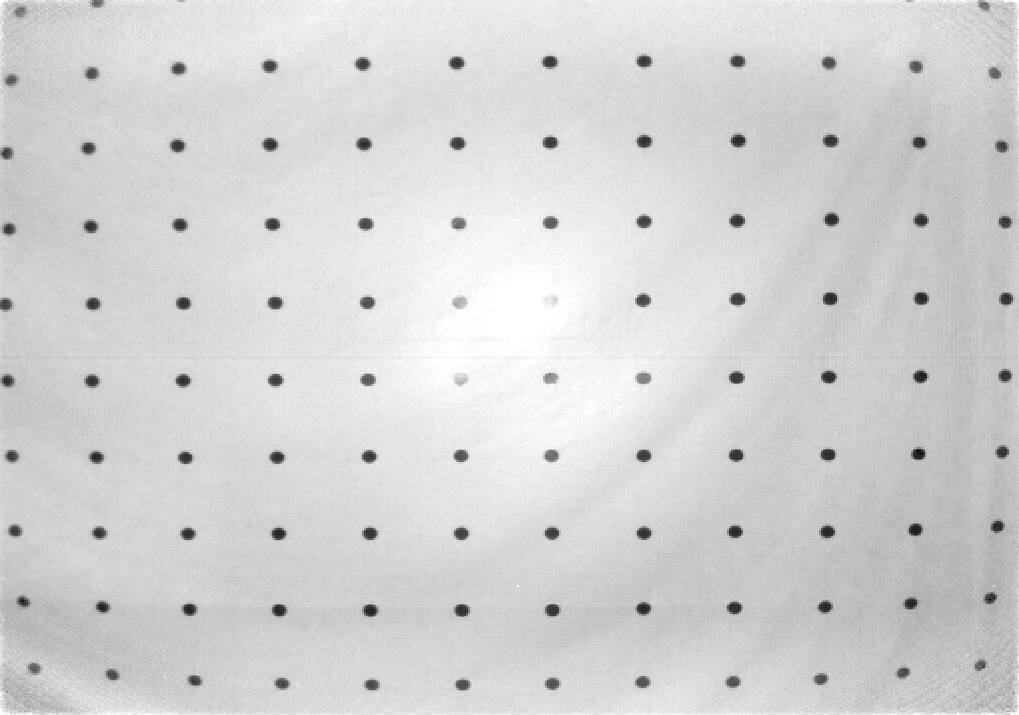
\includegraphics[width = 0.5\textwidth]{NIR_After_HistogramEqualization}
\label{NIR_After_HistogramEqualization_2}}
\subfloat[After Adaptive Thresholding][Binarized]{

\includegraphics[width=0.5\textwidth]{Binarized_Single_NIR}
\label{Binarized_Single_NIR}}%\qquad
\caption{NearIR Streams before / after Adaptive Thresholding}
\label{Adaptive_Thresholding}
\end{figure}%
%
There are three common types of blurring filters: mean filter, weighted average filter, and gaussian filter. Mean filter is selected for this background-aimed blurring process, because it has the smallest calculation and also a better effect of averaging than the others. After the blurred image containing background information is obtained, the binarizing (subtraction) process for every single pixel could be written as

\begin{equation}
%
Intensity_{\text{\_binarized}} = %
%
\begin{cases}
\,\, 1 , \quad \quad I_{\text{\_textured}} - I_{\text{\_background}}  -  C_{\text{\_offset}} \,\, > \,\,0 %
\\%
\,\, 0 , \quad \quad \quad \quad else%
\end{cases}
 \, ,%
\end{equation}%
%
where \(I\) is short for \(Intensity\) of every single pixel, and \(C_{\text{\_offset}}\) is a small constant that could be adjusted depending on various thresholding situations. In this project, \(C_{\text{\_offset}}\) is around 0.1.%
%
To sharpen the edge of the binarized image for a better \enquote{circle} shape detection, a median filter could be added as the last step of adaptive thresholding. As shown in Fig.~\ref{Adaptive_Thresholding}, background is removed in the binarized image after adaptive thresholding.
\\\indent
%
%
% Sniffer for Round Dot Center
After the adaptive thresholding, image data saved on GPU is now composed of circle-shaped \enquote{0}s within a background of \enquote{1}s. In order to locate the center of those \enquote{0}s circle, which is the center of captured round dot, it is necessary to know the edge of those circles. A trick is used to turn all of the edge data into markers that could lead a pathfinder to retrieve circle information.%
%
The idea that helps to mark edge data is to reassign pixels' values (intensity values) based on their surroundings. Using letter \(O\) to represent one single pixel in the center of a $3\times3$ pixels environment, and letters from \(A\)\texttildelow \(H\) to represent surroundings, a mask of 9 cells for pixel value reassignment could be expressed as below.

\begin{center}
  \begin{tabular}{ | c | c | c | }
    \hline
    \(E\) & \(A\) & \(F\) \\ \hline
    \(B\) & \(O\) & \(C\) \\ \hline
    \(G\) & \(D\) & \(H\) \\
    \hline
  \end{tabular}
\end{center}
%
To turn the surroundings \(A\)\texttildelow \(H\) into marks, different weights will be assigned to them. Those markers with different weights have to be non-zero data, and should be counted as the edge-part of circles. Therefore, the first step is to inverse the binary image, generating an image that consists of circle-shaped \enquote{1}s distributed in a background of \enquote{0}s.%
%
After reversing, the next step is to assign weight to the surroundings. OpenGL offers convenient automatic data type conversion, which means the intensity values from \enquote{0} to \enquote{1} of single-floating data type save on GPU could be retrieved to CPU as unsigned-byte data type from \enquote{0} to \enquote{255}. Considering a bitwise employment of markers, a binary calculation related weight assignment is used in the shader process for pixels. The intensity reassignment for every single pixel is expressed as the equation below.
%
\begin{equation}
\hspace*{-0.1cm}%
%
I_{\text{\_Path Marked}} = I_{\text{\_Original}} * \frac{(128I_{\text{A}} + 64I_{\text{B}} + 32I_{\text{C}} + 16I_{\text{D}} + 8I_{\text{E}} +  4I_{\text{F}} +  2I_{\text{G}}+I_{\text{H}})}{ 255 }
%
\label{snifferDistributionWeight}
\end{equation}%
\indent%
After this reassignment, the image is not binary any more. Every non-zero intensity value contains marked information of its surroundings, data at the edge of circles are now turned into fractions. In other words, the image data saved on GPU at the moment is composed of \enquote{0}s as background and \enquote{non-zero}s circles, which contains fractions at the edge and \enquote{1}s in the center.%
%
Now, it is time to discover dots through an inspection over the whole path-marked image, row by row and pixel by pixel. Considering that, a process of one single pixel in this step may affect the processes of the other pixels (which cannot be a parallel processing), it is necessary to do it on CPU. The single-floating image data will be retrieved from GPU to a buffer on CPU as unsigned-byte data, waiting for inspection. And correspondingly the new CPU image will have its \enquote{non-zero}s circles composed of fractions at the edge and \enquote{1}s in the center. Whenever a non-zero value is traced, a dot-circle is discovered and a singular-dot analysis could start. The first non-zero pixel will be called as an anchor, which means the beginning of a singular-dot analysis. %
%
During the singular-dot analysis beginning from the anchor, very connected valid (non-zero) pixel will be a stop, and a \enquote{stops-address} queue buffer is used to save addresses of both visited pixels and the following pixels waiting to be visited. On very visit of a pixel, there is a checking procedure to find out valid (non-zero) or not. Once valid, the following two steps are waiting to go. The first step is to sniff, looking for possible non-zero pixels around as the following stops. And the second step is to colonize this pixel, concretely, changing the non-zero intensity value to zero. Every non-zero pixel might be checked 1\texttildelow 4 times, but will be used to sniff for only once.%
\\\indent%
As for the sniffing step, base on the distribution table of \(A\)\texttildelow \(H\) that has been discussed above and their corresponding weight given by equation \ref{snifferDistributionWeight}, the markers \(A\)/\(B\)/\(C\)/\(D\) are valid (non-zero) as long as the intensity value of pixel \(O\) satisfies the following conditions shown as below.%
%
\begin{equation*}
%
\begin{aligned}
if \,\, ( I_{\text{O}} \,\, \& \,\, \text{0x80}  == 1 ),\quad &then, \quad \text{marker } A\,\, \text{is valid \,\,( go Up )}%
\\%
if \,\, ( I_{\text{O}} \,\, \& \,\, \text{0x40}  == 1 ),\quad &then, \quad \text{marker } B\,\, \text{is valid \,\,( go  Left)}%
\\%
if \,\, ( I_{\text{O}} \,\, \& \,\, \text{0x20}  == 1 ),\quad &then, \quad \text{marker } C\,\,\text{is valid \,\,( go Right )}%
\\%
if \,\, ( I_{\text{O}} \,\, \& \,\, \text{0x10}  == 1 ),\quad &then,\quad \text{marker } D\,\,\text{is valid \,\,( go Down )}%
\\%
\end{aligned}
%
\end{equation*}%
%
\noindent
Once a valid marker is found, its address \((column, row)\) will be saved into the \enquote{stops-address} queue. One pixel's address might be saved for up to 4 times, but \enquote{colonizing} procedure will only happen once at the first time, so that the sniffing will stop once all of the connected valid pixels in a singular dot-cluster are colonized as zeros.%
%
 \begin{figure}[t]
\hspace*{-0.5cm}
\centering
\subfloat[After Adaptive Thresholding][before Extraction]{

\includegraphics[width=0.5\textwidth]{Binarized_Single_NIR}
\label{Binarized_Single_NIR}}
%\qquad
\subfloat[Dot Centers Extraction][Extracted and Marked]{
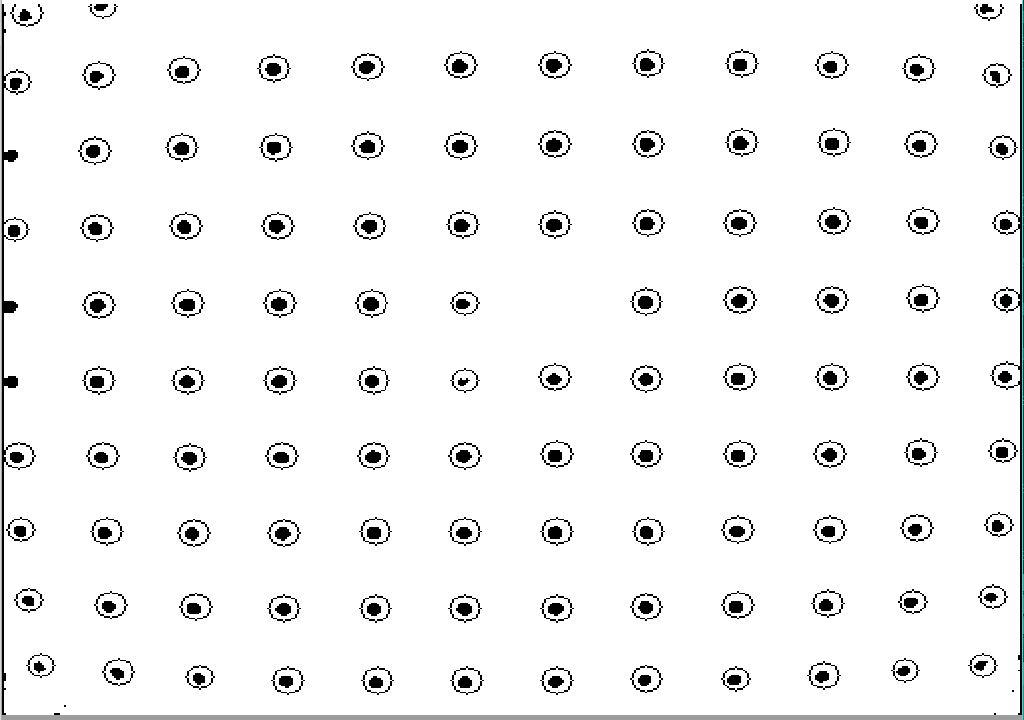
\includegraphics[width = 0.5\textwidth]{Dots_Extracted_Single_NIR}
\label{Dots_Extracted_Single_NIR}}
%
\caption{Valid Dot-Clusters Extracted in NearIR}
\label{DotCentersExtraction}
\end{figure}
%
In the second step \enquote{colonizing},  \(I_{\text{O}}\) is changed to zero, variable \(area\) of this dot-cluster pluses one, and bounding data \(RowMax\) / \(RoxMin\) / \(ColumnMax\) / \(ColumnMin\) are also updated.%
%
Finally, the Round Dot Centers \((column, row)\) could be determined as the center of bounding boxes with their borders \(RowMax\) / \(RoxMin\) / \(ColumnMax\) / \(ColumnMin\). After potential noises being removed based on their corresponding \(area\) and \(shape\) (ratio of width and height), the data left are taken as valid dot-clusters. As shown in Fig.~\ref{Dots_Extracted_Single_NIR}, the centers of valid dot-clusters are marked within their corresponding homocentric circles.
%%
%%
%%
\subsection{\((X^W, \,Y^W)\) Fitting based on Uniform Grid}
\label{uniformGridFittingXY}
%%
With a list of image space points (\(R, C\))s extracted, the following is to assign those points with their corresponding world coordinates \((X^W, \,Y^W)\)s, so that we can get coordinate-pairs to train a mapping model for dense \(X^WY^W\) generation. The world coordinates are based on the uniform grid. Taking the side of unit-square (distance between two adjacent dots) as \enquote{Unit One} in the world coordinates and one dot as the origin of plan \(X^WY^W\), all fitted \(X^W\)/\(Y^W\) values will be integers. %
\\\indent%
Ideally, a $3\times3$ perspective transformation matrix could help set a linear mapping between two different 2D coordinates, and 3 dot centers with known coordinates pair of \((R, C)\) and \((X^W, \,Y^W)\) are enough to determine the transformation matrix. Once four points with a squared-shape \(R\)/\(C\) distribution is found, a $3\times3$ perspective transformation matrix \(A\) could be determined by solving 
\begin{equation}
%
\left[ \begin{array}{c} %
zX^W \\ zY^W \\ z \end{array} \right] %
= %
A \left[ \begin{array}{c} %
C \\ R \\ 1 \end{array} \right] %
= %
\begin{bmatrix} 
a_{11} & a_{12} & a_{13} \\
a_{21} & a_{22} & a_{23} \\
a_{31} & a_{32} & a_{33} \\
\end{bmatrix}%
 \left[ \begin{array}{c} %
C \\ R \\ 1 \end{array} \right] %
%
\label{perspectiveDistortionCorrectionEquation}
\end{equation}%
%
\noindent
where \(C\) and \(R\) are vectors consist of four squared-shape distributed points' addresses; \(X^W\) and \(Y^W\) are vectors consist of four points \((0, 0)\), \((0, 1)\), \((1, 1)\), and \((1, 0)\); \(z\) denotes the third axis in the homogenous system connecting two coordinates. %
\\\indent%
Deformed by lens distortions, the cluster centers in image plane are not uniformly distributed, and this $3\times3$ transformation matrix can only generate corresponding decimal \(X^W\)/\(Y^W\) values that are close integers. But in practice, the correct integer values \(X^W\)/\(Y^W\) could still be located through \(Rounding\). Considering that a list of cluster centers' image coordinate \((R, C)\)s will give many groups of four squared-shape distributed points, and each of them gives a different image coordinate distance will be mapped to the \enquote{Unit One} in world coordinates, we will traverse all of the possible groups of four squared-shape distributed points and pick out the group whose mapping matrix \(A\) generates the most points that are close to integers. %
%
In this way, we find the transformation matrix \(A\) can give the best \enquote{Unit One} distance in world coordinates. However, its generated point \(X^W/Y^W = 0\) is usually not at the dot-cluster that is closest to the center of cameras' FoV. A translation matrix \(T\) could be used to refine the transformation matrix \(A\) and help to translate the origin point to be at the dot cluster we want, given by%
%
\begin{equation}
%
A_{\text{\_refined}}%
= %
T \cdot A %
= %
\begin{bmatrix} 
1 & 0 & -X_{\text{\_Zero\_A}} \\%
0 & 1 & -Y_{\text{\_Zero\_A}} \\%
0 & 0 &   1 \\%
\end{bmatrix}%
\cdot A%
\, \, \, ,%
\end{equation}%
%
where the integer world coordinate point \((X_{\text{\_Zero\_A}}, \, Y_{\text{\_Zero\_A}})\) are rounded world space coordinates, written as%
%
\begin{equation}
%
\left[ \begin{array}{c} %
zX_{\text{\_Zero\_A}} \\ zY_{\text{\_Zero\_A}} \\ z \end{array} \right] %
= %
A\cdot \left[ \begin{array}{c} %
C_{\text{\_center}} \\ R_{\text{\_center}} \\ 1 \end{array} \right] %
%
\end{equation}%
\noindent
which are mapped from the center point \((C_{\text{\_center}}, \, R_{\text{\_center}})\) of FoV in image plane by the transformation matrix \(A\). Eventually, the refined transformation matrix eventually generates a list of world coordinate points \((X^W, \, Y^W)\)s that correspond to image coordinates \((column, row)\)s. As shown in Fig.~\ref{XY_GridFitting_Matlab}, world coordinates are integers and the origin (blue circle) is chosen as where the center-closest dot-cluster is sitting.%
%
 \begin{figure}[t]
\hspace*{-0.3cm}
\centering
\subfloat[Image Plane Coordinates][ImagePlane Coordinate]{
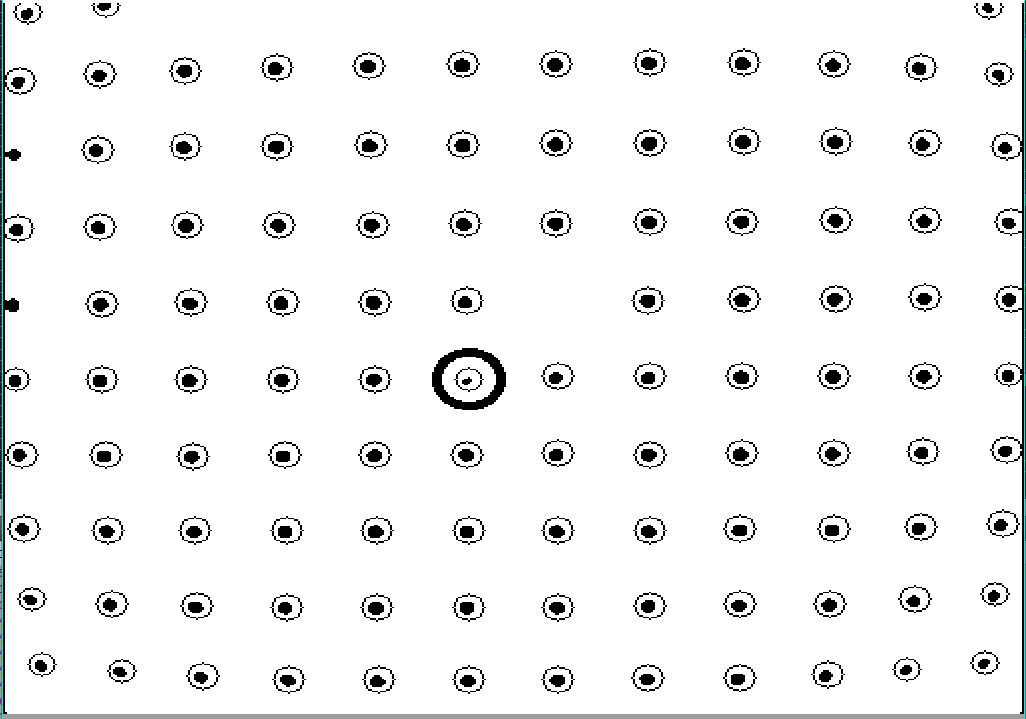
\includegraphics[width=0.54\textwidth, height = 0.425\textwidth]{Grid_Centered_Single_NIR}
\label{Grid_Centered_Single_NIR}}
%\qquad
\subfloat[World Coordinates][World Coordinate]{
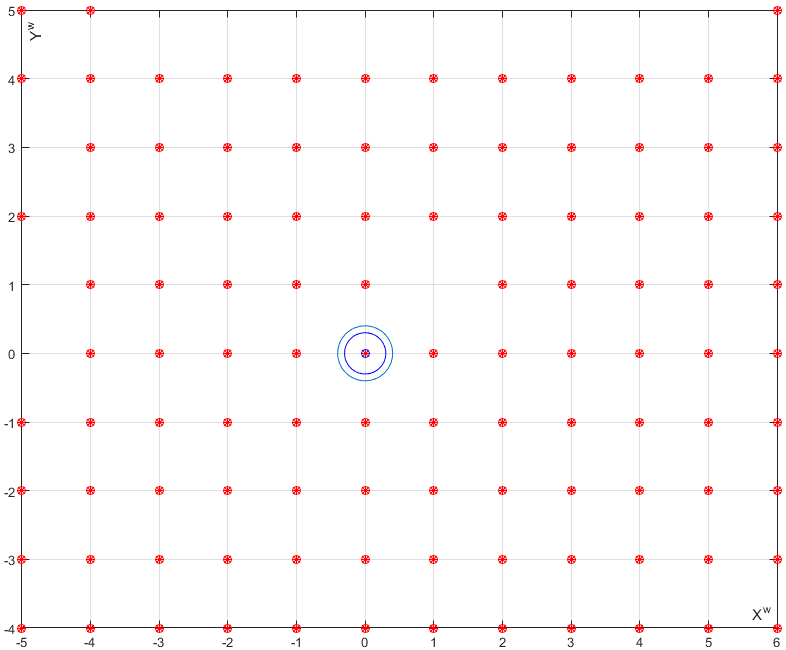
\includegraphics[width = 0.47\textwidth, height = 0.425\textwidth]{XY_GridFitting_Matlab}
\label{XY_GridFitting_Matlab}}
%
\caption{Coordinates-Pairs: (\(R, C\))s and (\(X^W\), \(Y^W\))s}
\label{Grid_Fitting}
\end{figure}%

%%
\subsection{Dense \(X^W/Y^W\) Generation}
\indent
%With a list of points with image space addresses (\(R, C\))s extracted,   
The generation of undistorted dense \(X^WY^W\) needs to consider lens distortion removal. In the traditional calibration method, world space \(X^\text{W}/Y^\text{W}/Z^\text{W}\) are mapped to undistorted (\(R', C'\)) by linear pinhole camera matrix \(M\). And then the undistortion step from undistorted (\(R', C'\)) to distorted (\(R, C\)) is done by eqn.~(\ref{lensDistortion}), which uses a high order (higher than 2nd order) polynomial equation. Assuming that there is a high order mapping relationship directly from the distorted image space (\(R, C\)) to world space (\(X^\text{W}, \, Y^\text{W}\)), we will do different orders of two-dimensional polynomial prototypes in Matlab using its application of \enquote{Curve Fitting Toolbox}, and then decide a best-fit mapping model with a high accuracy and a relative small number of parameters.
%
\\\indent
A two-dimensional polynomial model means surface mapping between two different spaces. Equation.~(\ref{perspectiveDistortionCorrectionEquation}) (perspective correction) as \(1^{st}\) order polynomial mapping is not able to handle lens distortions. 
%
The second order polynomial mapping has $2\times6=12$ parameters, written as %
%
\begin{equation}
\begin{aligned}
X^W &=  a_{11}C^2 + a_{12}CR + a_{13}R^2 + a_{14}C + a_{15}R + a_{16}
\\%
Y^W &=  a_{21}C^2 + a_{22}CR + a_{23}R^2 + a_{24}C + a_{25}R + a_{26} \, , 
\end{aligned}
\label{secondOrderPolynomial}
\end{equation}%
%
\noindent
and similarly, the fourth order polynomial mapping has $2\times15=30$ parameters, given by 
%
\begin{equation}
\hspace*{-0.3cm}%
\begin{aligned}
X^W &=  a_{11}C^4 + a_{12}C^3R + a_{13}C^2R^2 + a_{14}CR^3 + a_{15}R^4 + a_{16}C^3 + a_{17}C^2R \ \ \ ...\\%
&\,\,\,\,\,\,+ a_{18}CR^2 + a_{19}R^3 + a_{110}C^2 + a_{111}CR + a_{112}R^2 + a_{113}C + a_{114}R + a_{115}
\\\\%
Y^W &=  a_{21}C^4 + a_{22}C^3R + a_{23}C^2R^2 + a_{24}CR^3 + a_{25}R^4 + a_{26}C^3 + a_{27}C^2R \ \ \ ...\\%
&\,\,\,\,\,\,+ a_{28}CR^2 + a_{29}R^3 + a_{210}C^2 + a_{211}CR + a_{212}R^2 + a_{213}C + a_{214}R + a_{215}      \,\,.
\end{aligned}
\label{fourthOrderPolynomial}
\end{equation}%
%
\indent
To prototype equation \ref{secondOrderPolynomial} and \ref{fourthOrderPolynomial} in Matlab, \enquote{Curve Fitting Toolbox} is used to obtain the $2\times6$ and $2\times15$ parameters, using 107 points' coordinates pairs of image space \(R/C\) and world coordinates \(X^W/Y^W\). Based on the \enquote{Goodness of fit} of transformation parameters from Matlab, the Root-Mean-Square Error (RMSE) of (\(X^W\), \(Y^W\)) is (0.06796, 0.05638) for the \(2^{nd}\) order polynomial, and (0.02854, 0.02343) for the \(4^{th}\) order polynomial. As the order of polynomial goes higher, the RMSE gets smaller, and the cost of parameters' calculation gets much higher as well. After the prototyping in Matlab, the different orders of polynomial models will be applied into real-time streams transformation to get live transformed world space reconstruction. Eventually, the \(4^{th}\) order polynomial transformation model is selected as the distortion removal mapping model, which can give an intuitive undistorted world space image while costing relative less calculations. This mapping model will be trained by coordinate-pairs of the extracted points, and then be applied to image space addresses to generate dense \(X^W/Y^W\) for all pixels.
%% mapping model parameters determination
%
%
\section{Data Process and LUT Generation}
Till now, we have collected frames of \(X^WY^WZ^WRGBD\) data from RGB streams and \(X^WY^WZ^WID\) from NearIR stream. The \(X^WY^WZ^WRGBD\) data from RGB streams can be used for color values' alignment after the 3D reconstruction based on depth stream. Since the NearIR stream has same pixel distribution with depth stream, we will process the \(X^WY^WZ^WID\) data and generate per-pixel mapping parameters, which can be saved as LUT for undistorted 3D reconstruction. From section \ref{sectionRailCalibrationSystem}, we know that our whole idea of a calibrated natural 3D reconstruction on GPU is to make use of per-pixel eqn.~(\ref{kaiBeamEquationCh3}), which requires undistorted \(X^WY^WZ^W\) data and a per-pixel mapping from \(D\) to \(Z^W\). With enough \(X^WY^WZ^WID\) data already been collected, we will determine a per-pixel \(D\) to \(Z^W\) mapping, and then generate LUT for calibrated 3D reconstruction.
\\\indent
\begin{figure}[t]
\centering
\includegraphics[width=0.55\textwidth]{ZD_CurveFitting}
\caption{Polynomial Fitting between D and \(Z^W\)}
\label{ZD_CurveFitting}
\end{figure}%
%
Both of \(D\) and \(Z^\text{W}\) are continuous data, so that their function could written as a polynomial expression, based on Taylor series. We will determine a best-fit mapping model from \(D\) to \(Z^\text{W}\) using Matlab. Figure~\ref{ZD_CurveFitting} shows the polynomial fitting result in Matlab \enquote{Curve Fitting Tool} toolbox, with 32 points of \(DZ^\text{W}\) values (at pixel \(column\)=256 and \(row\)=212) from 32 frames. It is apparent that \(Z^\text{W}\) is linear with \(D\). Therefore, for every single pixel, \(Z^\text{W}\) could be mapped from \(D\) through \par
%
\begin{equation}
Z^W[m, \, n] = e[m, n]D[m, \, n]+f[m, n] ,
\label{fromD_To_Z}
\end{equation}%
%
\noindent
where \([m, \, n]\) denotes the image address \(Row\) and \(Col\) of a pixel, \(e/f\) are the corresponding linear coefficients that help map from \(D\) to \(Z^\text{W}\). With eqn.~(\ref{fromD_To_Z}) supporting the per-pixel \(Z^W\) values and eqn.~(\ref{kaiBeamEquationCh3}) help generating the per-pixel \(X^WY^W\) values, we found all of the six per-pixel parameters \((a/b/c/d/e/f)\) we need. We are now ready to process the collected data off-line and generate a \(numDepthRows\) by \(numDepthCols\) by 6 LUT.
\\\indent
%
 \begin{figure}[t]
\hspace*{-0.5cm}
\centering
\subfloat[Staggered]{
\includegraphics[width=0.5\textwidth]{staggeredPiles}
\label{staggeredPiles}}
%\qquad
\subfloat[Unified]{
\includegraphics[width = 0.5\textwidth]{unifiedPiles}
\label{unifiedPiles}}
%
\caption{World Space Unification of Collected Data}
\label{worldSpaceDataUnification}
\end{figure}
%
The collected data cannot be used directly for LUT generation, because \(X^W/Y^W\) may not be well aligned and pre-processes of data are needed. Our calibration system did not require the camera's observing orientation to be along with \(Z^W\)-axis, which results to the fact that, the collected frames might be staggered when the centered dot-cluster in camera's FoV moves. Figure~\ref{staggeredPiles} shows the raw collected data before world space unification, which has a staggered piles of frames. In order to make the data available for generating valid per-pixel 3D reconstruction parameters, we need to unify their world space by adding or subtracting a corresponding integer to all pixels in every staggered frame, making sure the point \(X^WY^W = 0\) is at the same dot-cluster for all frames.	After the data unification of world space, as shown in Fig.~\ref{unifiedPiles}, we are all ready to determine the per-pixel mapping parameters \(a/b/c/d/e/f\) and generate the LUT.
%\subsection{Mathematical tools}
%\subsubsection{Singular Value Decomposition (SVD)}
%\subsubsection{Least Square with Pseudo-Inverse}
%
\section{Alignment of RGB Pixel to Depth Pixel}
Now an undistorted 3D reconstruction could be displayed with the help of the calibrated LUT. However, we have not figured out yet what the color of each pixel is. To generate a colored 3D reconstruction with a combination of a random depth sensor and a random RGB sensor, we need to align the RGB pixels to depth pixels. The intermediate between the depth sensor image space and RGB sensor image space is the world space. As long as we figure out the mapping from world space to RGB sensor image space, the color of pixel with known \(X^WY^WZ^W\) could be looked up from the RGB image space. The pinhole camera matrix \(M\) is used to map from world space to RGB image space. Using the frame data from Kinect RGB steams and Kinect NearIR streams, a Matlab prototype of RGB pixels alignment is shown in Fig.~\ref{RGBAligned_Matlab}, where the RGB textured is mapped onto its corresponding NearIR image, who has same pixels with depth sensor. The total black area on the top edge and bottom edge is where the depth sensor's view goes beyond the RGB sensor's view. Figure~\ref{RGBAligned_Qt} shows the screen-shot of live video after calibration with the RGB pixels aligned by a pinhole camera model \(M\).

%
 \begin{figure}[t]
\hspace*{-0.5cm}
\centering
\subfloat[][]{
\includegraphics[width = 0.5\textwidth]{RGBAligned_Matlab}
\label{RGBAligned_Matlab}}
\subfloat[][]{
\includegraphics[width=0.5\textwidth]{RGBAligned_Qt}
\label{RGBAligned_Qt}}
\caption{Alignment of RGB Texture onto NearIR Image}
\label{Adaptive_Thresholding}
\end{figure}%
%

%	
%%	
%\section{Summation}
%A per-pixel calibration method, using a moving plane calibration system, is proposed in this chapter. The main idea of this calibration method is to make it available to generate accurate (undistorted) per-pixel world space position (\(X^W, \, Y^W, \, Z^W\)) directly in real-time with the fewest calculation. The per-pixel \(Z^W\) will be mapped from per-pixel depth value \(D\), and then per-pixel \(X^W/Y^W\) will be determined by per-pixel linear beam equation from its corresponding \(Z^W\). Note that the per-pixel beam equation represents the lens-distortion removed field of view of a single pixel. And the \enquote{depth distortion} could be removed during the per-pixel mapping from \(D\) to \(Z^W\). In short, this per-pixel calibration method consists of two big steps: \(X^WY^WZ^W+D\) data collection and mapping parameters determination. \(D\) is simply from depth streams. \(Z^W\) is from external based on the camera's position on the rail. And the undistorted (\(X^W, \, Y^W\)) are from the transformation of \(R/C\) by a \(4^{th}\) order polynomial mapping model, during which lens-distortions could be removed. With the frames data of \(X^WY^WZ^W+D\) collected, the per-pixel mapping parameters \(a/b/c/d/e/f\) could be determined by eqn.~(\ref{fromD_To_Z}) and eqn.~(\ref{kaiBeamEquationCh3}). 
%\\\indent
%Without using the traditional pinhole camera model, two polynomial mapping models are employed in this calibration method. The first model is the two-dimensional \(4^{th}\) order polynomial mapping from \(R/C\) to \(X^W/Y^W\) during the frames data collection, which takes care of the removal of lens distortions; and the second model is the linear mapping from \(D\) to \(Z^W\), which can handle \enquote{depth distortion}. Both of the two mapping models are determined and calculated by real streams data from the camera, so that we claim this per-pixel calibration method a \enquote{data-based} calibration method. 
%\\\indent
%Besides the data-based calibration method, a robust DIP process during calibration is also discussed, which guarantees that the live video during undistorted frames collection could be in real-time. Note that \enquote{real-time} here means being able to show an undistorted frame before the start of the second frame processing. After the undistorted 3D reconstruction, the alignment of the RGB pixel to Depth pixel is also discussed. The data-based calibration method could be applied universally on any RGB-D cameras. With the alignment of RGB pixels, it could even work on the combined 3D camera of a random Depth sensor and a random RGB sensor.

















%
%
% Kai \cite{Kai10} shows that, GPU programing is ideally suited to this kind of per-pixel processing. He did a good job on structed light 3D scanner parallel calibration on GPU, and derived the per-pixel beam equation~(\ref{kaiBeamEquationCh3}) directly from a pinhole camera matrix \(M\). 
%%
%\begin{equation}
%\begin{aligned}
%X^W[m,\,  n] = c[m, n]Z^W[m,\,  n]+d[m, n]
%\\%
%Y^W[m,\,  n] = e[m, n]Z^W[m,\,  n]+f[m, n]
%\end{aligned}
%\label{kaiBeamEquationCh3}
%\end{equation}%
%\noindent
%where [\(m,n\)] is the discrete space \(row\) and \(column\) coordinate of each pixel in a M by N sensor. This per-pixel beam equation shows per-pixel linear mappings from \(Z^W\) to \(X^W/Y^W\), and the per-pixel \(Z^W\) can be mapped from features of structured light. 
%\\\indent
%Without calibration, we can also derive per-pixel beam equations in camera space and apply them in GPU parallel processing. In this section, we will introduce how to draw a colored camera space 3D reconstruction on GPU without calibration, using a KinectV2 camera. As shown in the diagram in Fig.~\ref{cameraSpaceDiagram}, we will retrieve \(Depth\), \(RGB\) and \(mapping\) streams from the KinectV2 camera, and save them into corresponding buffers respectively. The mapping streams contains \(Row\) and \(Column\) values that can help every depth pixel to look for color infos from \(RGB\) streams. Then those three streams will be uploaded from CPU onto GPU as textures for image drawing. The camera space 3D coordinates \(X^CY^CZ^C\) for the final 3D image will be generated based on depth texture, which will also be processed on GPU in the way that similar to drawing colors on a pixel. In short, we will draw on GPU twice: one for camera space coordinates generation and \(RGB\) alignment, the other one for real 3D image drawing.
%\\\indent
%
%In the first drawing step of camera space coordinates generation, a look-up texture will be created for the final 3D image drawing, which contains both camera space coordinates and color (RGB) values. To draw a certain color on one single pixel, GPU provide one single fragment shader to generate and save corresponding four color channel RGBA (A for alpha, opacity) single-floating data into a corresponding position in a framebuffer. We could take the framebuffer as a screen on which we are going to draw, and the positions in the framebuffer would be same with pixels in the screen. We will follow the way how GPU do drawing, and use GPU to calculate per-pixel \(X^CY^CZ^C\) and save the calculation results with RGB streams together as total six channels into a customer framebuffer. The first thing is to initial a customer framebuffer, whose texture will finally be utilized to look up per-pixel's \(X^CY^CZ^CRGB\) six channels of data for the eventual 3D image drawing. The internal texture format of {\ttfamily\color[rgb]{0.0,0.0,0.5019608}GL\_RGBA32F}, which means one pixel position (\(row\), \(column_0\)) can contain four channels. We need a second position (\(row\), \(column_0 + 1\)) for every single pixel to contain the total six channels. Therefore the customer framebuffer will be initialed with a size of %
%({\ttfamily
%\textcolor[rgb]{0.0,0.0,0.5019608}{2}\textcolor{black}{* }\textcolor[rgb]{0.5019608,0.0,0.0}{numDepthCols}\textcolor{black}{, }\textcolor[rgb]{0.7529412,0.7529412,0.7529412}{
% }\textcolor[rgb]{0.5019608,0.0,0.0}{numDepthRows}}),
%where numDepthRows and numDepthCols denote the size of total rows and total columns of the depth sensor. %
%\\\indent
%Four corner points coordinates, as four vertices, will be uploaded onto vertex shader to form a quadrilateral filling up the screen, which will cover the numDepthRows by (2*numDepthCols) framebuffer. With respect to a random position of every single depth pixel, two corresponding \enquote{virtual pixels} (positions) will be processed by two independent fragment shaders to respectively save \(X^CY^CZ^C\) and \(RGB\) data into the customer framebuffer. The fragment shader is programmed as below.
%\\%
%%
%This fragment shader handles both of \(X^CY^CZ^C\) generation and \(RGB\) texel fetch. There are four uniform input textures uploaded on GPU. The \emph{qt\_colorTexture} is RGB stream, and \emph{qt\_depthTexture} is depth stream. \emph{qt\_mappingTexture} is a mapping stream also given by KinectV2 camera, which contains two channels \(Row/Col\) mapping data. It offers a link between RGB stream and Depth stream, helping align RGB values to depth pixels. \emph{qt\_spherTexture} is a per-pixel beam mapping texture created by ourselves, which helps map from \(Z^C\) to \(X^C/Y^C\) respectively based on the horizontal and vertical field of view of a pinhole camera model. Let's view the fragment shader step by step, and then talk about the creation of beam mapping texture in detail.%
%\\\\
%We will first get the texture coordinates from the fragment coordinates.
%\\\\
%    ivec2 textureCoordinate = ivec2(gl\_FragCoord.x/2, gl\_FragCoord.y);
%\\\\
%And then have a check if this fragment shader should be assigned for \(X^CY^CZ^C\) generation, or \(RGB\) texel fetch.\\\\
%    if (int(gl\_FragCoord.x)\%2 == 0)\{\\
% 		// \(X^CY^CZ^C\) generation
%    \} else \{
%		// \(RGB\) texel fetch
%    \}%
%%
%\\\\
%The depth steam measures \(Z^C\), which after rescaling is given by :
%\\\\
%        float z = texelFetch(qt\_depthTexture, ivec2(col, textureCoordinate.y), 0)[chn] * 65130.0 - 20.0;
%\\\\
%
%Based on the pinhole-camera model, we could derive a per-pixel proportional mapping from \(Z^C\) to \(X^C/Y^C\) using the horizontal and vertical Field of View. In a depth sensor of size %
%({\ttfamily
%\textcolor[rgb]{0.5019608,0.0,0.0}{numDepthCols}\textcolor{black}{, }\textcolor[rgb]{0.7529412,0.7529412,0.7529412}{
% }\textcolor[rgb]{0.5019608,0.0,0.0}{numDepthRows}}),
%%
%a pixel with image address (\(Row, \, Col\)) has its view in camera space as a beam passing through the camera space origin (the pin hole). For one specific camera with a certain filed of view, a pixel's beam function depends on its address (\(Row, \, Col\)). As shown in Fig.~\ref{VHfieldOfView}, the relationship between a pixel's beam view (\(Z^C\) to \(X^CY^C\)) and the sensor's vertical / horizontal Field of View could be expressed as eqn.~(\ref{pinholeProportionZXY}).
%%
%\begin{equation}
%\begin{aligned}
%\frac{X^C_{[Row, \, Col]}}{Z^C_{[Row, \, Col]} \times tan(horFoV / 2)} 
%=
%%tan\bigg[
%%	Hor\text{FoV}
%%		\bigg(
%			\frac{Col}{numDepthCols} - 0.5
%%		\bigg)
%%\bigg]
%\\\\%
%\frac{Y^C_{[Row, \, Col]}}{Z^C_{[Row, \, Col]} \times tan(verFoV / 2)} 
%=
%%tan\bigg[
%%	Ver\text{FoV}
%%		\bigg(
%			\frac{Row}{numDepthRows} - 0.5
%%		\bigg)
%%\bigg]
%\end{aligned}
%\label{pinholeProportionZXY}
%\end{equation}%
%
%\noindent
%From eqn.~\ref{pinholeProportionZXY}, we could generate a per-pixel beam mapping texture which contains the proportion parameters that can map from per-pixel \(Z^C\) to per-pixel \(X^C/Y^C\).
%\\\\
%        vec4  a = texelFetch(qt\_spherTexture, textureCoordinate, 0);\\
%        // CONVERT SPHERICAL COORDINATES TO CARTESIAN\\
%        qt\_fragColor.x = -z * a.r;\\
%        qt\_fragColor.y = -z * a.g;\\\\































































%In our calibration system, 



%
%%%
%%%
%%%
%\indent From Chapter \ref{chapterTraditionalCalibration} we know one dimension calibration method is suitable for calibrating multiple cameras together; three dimension object calibration has the highest accuracy but also cost more on system setup; two dimension plane calibration owns both of good accuracy and simple setup. However, those traditional calibration methods are not ideal enough while considering that researchers are chasing after accuracy. Either that, the static calibration pattern does not have enough points to offer distortions' information. Concretely only few limited points could be extracted in the three dimension calibration system as shown in Fig.~\ref{threeDSixPointsCalibrating}. Or, it is hard to control the extracted calibration points to cover enough area of the image space in the famous two dimension calibration methods. Fig.~\ref{simulatedMultiPlanesCheckerboard} shows the simulated multiple planes of checkerboard with respect to the camera space, with data from the two dimension calibration method that is employed in both of Matlab and OpenCV applications, to intuitively inspect the extrinsic parameters. Using this method, researchers need to manually keep changing their poses of holding the checkerboard, in order to get enough calibration points to cover all of the image space area. Besides, all of the traditional calibration methods are assuming that the depth sensor offers perfect accurate \(Z^C\) values for all of its pixels, \textit{i.e.}, \(Z^C_{[row, col]} - Depth_{[row, col]} = E_{\text{Constant}}\) such that for all image space range of \([row,\, col]\) pixels  share one same error \(E_{\text{Constant}}\). But in practice, depth sensors always have some defects in getting same depth accuracy for all of their pixels, which we will call as \enquote{Depth Distortion}. As shown in Fig.~\ref{NIR_by_Depth_LeftSide}, even observing a flat wall there are still many bumps and hollows in the reconstructed 3D image.
%%
% \begin{figure}[b]
%%\hspace*{-0.5cm}
%\centering
%\includegraphics[width=0.55\textwidth]{simulatedMultiPlanesCheckerboard}
%\caption{Simulated Planes of Checkerboards showing Extrinsic Parameters}
%\label{simulatedMultiPlanesCheckerboard}
%\end{figure}%
%%
%%
%\\\indent
%Most of those defects in the methods discussed above are based on the losing control of the calibration points. Even though a flexible two dimension calibration method got its camera observing orientations easily changed by hand, it is almost impossible to numerically locate all desired poses that can make calibration points fill up all image space area. However, Tsai's old calibration system, which requires a known motion of the plane, can make them up. It has been obsoleted nowadays due to the fact that knowing the motion is not necessary for determining the intrinsic and extrinsic parameters. But as the resolution of camera sensor gets higher and higher, like a high definition sensor, researchers need a better calibration system. What's more, with the motion of the calibration plane controllable, it will not be a problem to determine the mapping from \(Depth (D)\) to \(Z^W\), thus equation \ref{kaiBeamEquation} could be applied as one important step to simplify 3D reconstruction using a look-up table (lut) after calibration. Note that, both of the mapping from \(D\) to \(Z^W\) and the coefficients \(c/d/e/f\) help map from \(Z^W\) to \(X^W/Y^W\) are with respect to per-pixel, such that even the \enquote{Depth Distortion} could be calibrated.
%
%\section{Novel Per-Pixel Calibration Method}
%\label{sectionPerPixelCalibration}
%In this thesis, we build a moving plane calibration system collecting tree dimensional data, with a rail that gets the RGB-D camera mounted on its slider observing a planar pattern. The 3D camera we used is KinectV2, but the calibration method could be applied on any RGB-D cameras. As shown in Fig.~\ref{trackingModuleOnKinectV2CalibrationSystem}, a uniform grid dots pattern is hung on the wall, and the rail is perpendicular to the wall. We will assign the wall, on which the canvas is hung and printed with uniform grid dots pattern, as the \(X^WY^W\) plane in world space, and \(Z^W\)-axis would be along the rail. The RGB-D camera waiting to calibrate is mounted on the slider. Note that, in this calibration system, the only unit that needs to be perpendicular to the wall is the rail, whereas the RGB-D camera has no need to require its observation orientation. Because all of the mappings we are going to determine are with respect to per-pixel, \textit{i.e.}, the calculated parameters group for every single pixel, which will determine the pixel's view, are independent with that of the other pixels. As the slider moves along the rail, the planar dots pattern hung on the wall is moving further with respect to the RGB-D camera. This rail offers the possibility of taking infinite various frames of various camera working distances (or \(Z^C\)). Although the dots pattern hung on the wall for camera calibration is static itself, however, the dots distributions would be dynamic (covering every single pixel) in the image space when counted together in all of those various frames of various \(Z^C\). 
%\\\indent%
%%how to per-pixel calibrate ?
%In this per-pixel calibration method, we directly focus on the view of every single pixel, the beam. Inspired by Kai (eqn.~\ref{kaiBeamEquation}), our camera calibration method consists of two big steps: frames (\(X^\text{W}Y^\text{W}Z^\text{W}+D\)) data collection, plus per-pixel mapping parameters determination after frames collection; \textit{i.e.}, to collect frames data of \(Z^\text{W}\) from external and (\(X^\text{W}, \, Y^\text{W}\)) by a transformation from (\(R, C\)), plus to calculate per-pixel parameters that help map from \(D\) to \(Z^\text{W}\) and \(c/d/e/f\) in eqn.~\ref{kaiBeamEquation} that map from \(Z^\text{W}\) to \(X^\text{W}/Y^\text{W}\). Note that, neither have we decided the mapping model from \(D\) to \(Z^\text{W}\), nor from (\(R, C\)) to (\(X^\text{W}, \, Y^\text{W}\)). We save the flexibilities between accuracy and complexity for now, and will decide those two models based on data.
%\\\indent%
%% World Coordinates assignment
%Assuming the total size of the depth sensor is as small as a point, and the \(Z^W\)s for all of the pixels in one frame would share the same value, which could be measured by a laser distance measurer nearby the camera. To simplify the digital image processing (DIP) when extracting a desired point (\(R,\, C\)), which will soon be discussed in section \ref{sectionDIPTechniques}, we assign the \enquote{2D origin} (\(X^\text{W}/Y^\text{W}\) = 0) of world space coordinates at the center of the dot which is closest to the center of the camera's field of view. And the laser measurer spot nearby the camera to at \(Z^\text{W}\)=0, such that \(Z^{W}\) values are always negative. Note that, the final assigned world space origin (\enquote{3D origin}) is not necessarily be where the camera sensor is. It depends on the camera's observation orientation, whose changing leads to the change of the \enquote{2D origin} (and finally change the 3D origin).
%%%Zw collection
%%%Zw collection
%%%Zw collection
%%%
%\\\\\indent
%In our calibration system, \(Z^{W}\) values for all pixels of every frame will be supported from external laser distance measurer. The \enquote{Unit One} of \(Z^{W}\) value is assigned to be same with the side of unit-square of the uniform grid pattern, which can simplify the DIP processing of (\(C, \, R\)) extraction. Concretely, the distance between every two adjacent dots' centers in real-world is 228mm. Therefore, \(Z^{W}\) = -\(Z\)(mm) / 228(mm), where \(Z\) is the distance in reality from the camera to dots-pattern plane along the rail. Fig.~\ref{OneFrameXYZ_Calibrated} shows one sample frame of 3D reconstruction in the assigned world space, where both of the origin and \(Z\)-axis are high-lighted in blue.
%%
%\begin{figure}[!t]
%\centering
%%calibrated \(X^{W}\)/\(Y^{W}\) and \(Z^{W}\)
%\includegraphics[width=0.7\textwidth, height= 0.5\textwidth]{OneFrameXYZ_Calibrated}
%\caption{NearIR \(X^{W}Y^{W}Z^{W}\) 3D Reconstruction}
%\label{OneFrameXYZ_Calibrated}
%\end{figure}%
%%
%%%
%%%XwYw collection
%%%XwYw collection
%%%XwYw collection
%%%
%\\\indent
%As for (\(X^\text{W}, \, Y^\text{W}\)) values' collection, a transformation from (\(R, C\)) is needed, during which the lens distortions correction must be considered. In the traditional calibration method, world space \(X^\text{W}/Y^\text{W}/Z^\text{W}\) are mapped to undistorted (\(R', C'\)) by linear pinhole camera matrix \(M\). And then the undistortion step from undistorted (\(R', C'\)) to distorted (\(R, C\)) is done by eqn.~\ref{lensDistortion}, which uses a high order (higher than 2nd order) polynomial equation. Assuming that there is a high order mapping relationship directly from the distorted image space (\(R, C\)) to world space (\(X^\text{W}, \, Y^\text{W}\)), we will do different orders of two-dimensional polynomial prototypes in Matlab using its application of \enquote{Curve Fitting Toolbox}, and then decide a best-fit mapping model with a high accuracy and a relative small number of parameters.
%%
%\\\indent
%A $3\times3$ linear transformation matrix \(A\) (as \(1^{st}\) order polynomial) is usually used for perspective distortion correction, give by eqn.~\ref{perspectiveDistortionCorrectionEquation}. We will try the perspective distortion correction to check if it will also work on the lens distortion correction.
%%
%\begin{equation}
%%
%\left[ \begin{array}{c} %
%zX^W \\ zY^W \\ z \end{array} \right] %
%= %
%A\cdot \left[ \begin{array}{c} %
%C \\ R \\ 1 \end{array} \right] %
%= %
%\begin{bmatrix} 
%a_{11} & a_{12} & a_{13} \\
%a_{21} & a_{22} & a_{23} \\
%a_{31} & a_{32} & a_{33} \\
%\end{bmatrix}%
%\cdot \left[ \begin{array}{c} %
%C \\ R \\ 1 \end{array} \right] %
%%
%\label{perspectiveDistortionCorrectionEquation}
%\end{equation}%
%%
%\noindent
%A two-dimensional polynomial model means surface mapping between two different spaces. The second order polynomial mapping has $2\times6=12$ parameters, written as %
%%
%\begin{equation}
%\begin{aligned}
%X^W &=  a_{11}C^2 + a_{12}CR + a_{13}R^2 + a_{14}C + a_{15}R + a_{16}
%\\%
%Y^W &=  a_{21}C^2 + a_{22}CR + a_{23}R^2 + a_{24}C + a_{25}R + a_{26} \, , 
%\end{aligned}
%\label{secondOrderPolynomial}
%\end{equation}%
%%
%\noindent
%and similarly, the fourth order polynomial mapping has $2 \times 15$=30 parameters, given by eqn.~\ref{fourthOrderPolynomial}.%
%%
%\begin{equation}
%\hspace*{-0.3cm}%
%\begin{aligned}
%X^W &=  a_{11}C^4 + a_{12}C^3R + a_{13}C^2R^2 + a_{14}CR^3 + a_{15}R^4 + a_{16}C^3 + a_{17}C^2R \\%
%&\,\,\,\,\,\,+ a_{18}CR^2 + a_{19}R^3 + a_{110}C^2 + a_{111}CR + a_{112}R^2 + a_{113}C + a_{114}R + a_{115}
%\\\\%
%Y^W &=  a_{21}C^4 + a_{22}C^3R + a_{23}C^2R^2 + a_{24}CR^3 + a_{25}R^4 + a_{26}C^3 + a_{27}C^2R \\%
%&\,\,\,\,\,\,+ a_{28}CR^2 + a_{29}R^3 + a_{210}C^2 + a_{211}CR + a_{212}R^2 + a_{213}C + a_{214}R + a_{215}
%\end{aligned}
%\label{fourthOrderPolynomial}
%\end{equation}%
%%
%\indent
%To prototype equation \ref{secondOrderPolynomial} and \ref{fourthOrderPolynomial} in Matlab, \enquote{Curve Fitting Toolbox} is used to obtain the $2\times6$ and $2\times15$ parameters, using 107 points' coordinates pairs of image space \(R/C\) and world coordinates \(X^W/Y^W\). Based on the \enquote{Goodness of fit} of transformation parameters from Matlab, the Root-Mean-Square Error (RMSE) of (\(X^W\), \(Y^W\)) is (0.06796, 0.05638) for the \(2^{nd}\) order polynomial, and (0.02854, 0.02343) for the \(4^{th}\) order polynomial. As the order of polynomial goes higher, the RMSE gets smaller, and the cost of parameters' calculation gets much higher as well. After the prototyping in Matlab, the different orders of polynomial models will be applied into real-time streams transformation to get live transformed world space reconstruction. Eventually, the \(4^{th}\) order polynomial transformation model is selected as the distortion removal mapping model, which can give an intuitive undistorted world space image while costing relative less calculations. Detailed results and comparisons will be shown soon in section~\ref{sectionPrototypeTwoDtransformation}.
%\\\\\indent
% %% mapping model parameters determination
%%
%\begin{figure}[b]
%\centering
%\includegraphics[width=0.55\textwidth]{ZD_CurveFitting}
%\caption{Polynomial Fitting between D and Z}
%\label{ZD_CurveFitting}
%\end{figure}%
%%
%Till now, the mapping model from (\(R, C\)) to (\(X^\text{W}, \, Y^\text{W}\)) has been decided, with which the data collection of \(X^\text{W}Y^\text{W}Z^\text{W}+D\) is ready to be completed. With enough data, the four per-pixel parameters in the beam equation \ref{kaiBeamEquation} are now able to be calculated. In the meanwhile, a best-fit mapping model from \(D\) to \(Z^\text{W}\) could also be determined. Both of \(D\) and \(Z^\text{W}\) are continuous data, so that their function could written as a polynomial expression, based on Taylor series. Fig.~\ref{ZD_CurveFitting} shows the polynomial fitting result in Matlab \enquote{Curve Fitting Tool} toolbox, with 32 points of \(DZ^\text{W}\) values (at pixel \(column\)=256 and \(row\)=212) from 32 frames. It is apparent that \(Z^\text{W}\) is linear with \(D\), which is also reasonable. Therefore, for every single pixel, \(Z^\text{W}\) could be mapped from \(D\) through \par
%%
%\begin{equation}
%Z^W_{[row, \, col]} = a_{[row, col]}D_{[row, \, col]}+b_{[row, col]} ,
%\label{fromD_To_Z}
%\end{equation}%
%%
%\noindent
%where \({[row, \, col]}\) denotes the address of a pixel, \(a/b\) are the corresponding linear coefficients that help map from \(D\) to \(Z^\text{W}\). With eqn.~\ref{fromD_To_Z} supporting the per-pixel \(Z^W\) values, eqn.~\ref{kaiBeamEquation} help generating the per-pixel \(X^WY^W\) values, all of the 3D camera's per-pixel calibration is now done, and we are all ready to show an undistorted 3D \(X^WY^WZ^W\) reconstruction image.
%%
%%
%%
%%
%\section{DIP Techniques on (\(R,\, C\)) Extraction}
%\label{sectionDIPTechniques}
%%  add noises analysis
%\noindent
%In order to train the \(4^{th}\) order mapping model that can map from (\(R, \, C\)) to (\(X^W, \, Y^W\)), we need to obtain at least 15 points' coordinate-pairs of both image space coordinates and world space coordinates. Therefore, a robust DIP process to extract the points' addresses (\(R,\, C\))s is of the top priority. Concretely in this project, we are going to extract the dot-clusters' centers from KinectV2 NearIR steams using DIP techniques. To guarantee a robust processing, the extraction steps consist of gray-scaling, histogram equalization, adaptive thresholding and a little trick on black pixels counting. OpenGL is selected as the CPU image processing language. The default data type of steams saved on GPU during processing is single-floating, with a range from 0 (balck) to 1 (white). 
%\\\indent
%Gray-scaling is done in order to suit for both of the RGB and the NearIR steams. For NearIR steam, its data contains only color gray. There is no need to consider gray-scale problem, and data will be saved on GPU as single-floating automatically. Whereas for RGB steam, a conversion from RGB to gray value is needed. Typically, there are three converting methods: lightness, average, and luminosity. The luminosity method is finally chosen as a human-friendly way for gray-scaling, because it uses a weighted average value to account for human perception, which is give by eqn.~\ref{luminosityGrayScaling}.
%\\\indent
%%
%\begin{equation}
%Intensity_{\text{\_gray}} =  0.21 Red\,  + \, 0.72 Green \, + \, 0.07 Blue
%\label{luminosityGrayScaling}
%\end{equation}%
%%
%As values saved on GPU, all of the pixel intensity values are within the range of [0, 1], where \enquote{0} means 100\% black and \enquote{1}  means 100\% white. In practice, NearIR steam image is always very dark, as shown in Fig.~\ref{Raw_Single_NIR} (with their intensity values every close to zero).  In order to enhance the contrast of NearIR image for a better binarizing, rescaling is necessary. In this section, histogram equalization technique is used maximize the range of valid pixel intensity distributions. Same process is also compatible on the RGB steam.
%%
% \begin{figure}[t]
%\hspace*{-0.5cm}
%\centering
%\subfloat[Raw NearIR][Raw]{
%\includegraphics[width=0.5\textwidth]{Raw_Single_NIR}
%\label{Raw_Single_NIR}}
%\subfloat[Histogram Equalized NearIR][Histogram Equalized]{
%\includegraphics[width = 0.5\textwidth]{NIR_After_HistogramEqualization}
%\label{NIR_After_HistogramEqualization}}
%%\qquad
%\caption{NearIR Streams before / after Histogram Equalization}
%\label{Histogram_Equalization}
%\end{figure}%
%%
%Commonly, Probability Mass Function (PMF) and Cumulative Distributive Function (CDF) will be calculated to determine the minimum valid intensity value (\(floor\)) and maximum valid value (\(ceiling\)) for rescaling, whereas tricks could be used by taking advantage of the GPU drawing properties.%
%\\\indent%
%PMF means the frequency of every valid intensity value for all of the pixels in an image. Dividing all of the pixels in terms of their intensity values into \(N\) levels, every pixel belongs to one level of them, which is called gray level. With an proper selection of \(N\) to make sure a good accuracy, the intensity value of a pixel could be expressed based on its gray level \(n\)
%%
%\begin{equation}
%Intensity = n/N * (1 - 0) + 0 = n/N \, ,
%\end{equation}%
%\noindent
%where \(n\) and \(N\) are integers and \(1 \leqslant n \leqslant N\).%
%%
%PMF calculation is very similar with the points-drawing process in terms of GPU that, both of them share the properties of pixel-by-pixel calculation. For the GPU points-drawing process onto a customer framebuffer, the single-floating \enquote{color} value could go beyond the normal range [0, 1], with a maximum value of a signed 32-bit integer (\(2^{31}\) - 1). And different \enquote{color} values will be added together to form a \enquote{summational-color} in the case that some pixels are drawn onto the same position coordinates. \enquote{Taking} the range of pixel intensity values [0, 1] \enquote{as} a segment on x-axis waiting to be drawn, the intensity frequency \enquote{as} the \enquote{summational-color} of multiple pixels with different intensity drawn at the same position, and the counting process of intensity frequency \enquote{as} a points-drawing process, PMF could be calculated by drawing all of the pixels onto the x-axis within the normal intensity range [0, 1], with every single pixel's position coordinates re-assigned as (\(pixel\_intensity\), \(0\)) and its \enquote{color} value constantly being equal to one. Given the width (range of x-axis) of customer framebuffer being [-1, 1] in OpenGL, which is twice the range of pixel intensity [0, 1], the half-width of the customer framebuffer is same with the total number \(N\) of gray levels, which determines the precision of \(floor\) / \(ceiling\) intensity selection. 
%\\\indent%
%With PMF calculated and each intensity frequency that mapped to its corresponding gray level saved in the customer framebuffer, CDF could be easily calculated as
%%
%\begin{equation}
%%
%CDF(n) = \frac{sum}{N_{\text{\_Total Pixels/Image}}} \, ,
%%\label{lensDistortion}
%%
%\end{equation}%
%%
%where the gray level \(n\) is counted from the middle of the framebuffer's width to the end (1 \texttildelow \, \(N\)). And \(sum\) is the summation of customer framebuffer's values added up consecutively from 1 till \(n\). %
%%
%Then, at appropriate CDFs, e.g., \(CDF(n_{\text{\_floor}}) = 0.01\) and \(CDF(n_{\text{\_ceiling}}) = 0.99\), the intensities \(floor\) and \(ceiling\) could be written as
%%
%\begin{equation}
%\begin{aligned}
%floor &=  n_{\text{\_floor}} / N%
%\\%
%ceiling &=  n_{\text{\_ceiling}} / N
%\end{aligned}
%\label{intensityFloorCeilingDetermination}
%\end{equation}%
%%
%\noindent
%Finally, a new intensity value of every single pixel in an image could be rescaled as
%%
%\begin{equation}
%Intensity_{\text{\_new}} = \frac{Intensity_{\text{\_original}} - floor}{ceiling - floor} 
%\end{equation}%
%%
%\noindent
%After this final rescaling step of Histogram Equalization, the new image gets better contrast effect, as shown in Fig.~\ref{NIR_After_HistogramEqualization}%
%\\\\\indent%
%%% Adaptive Thresholding
%Affected by radial dominated lens distortions, the intensity value tend to decrease as the position of a pixel moves from the center of an image to the borders, in the case of observing a singular color view. Therefore, an adaptive thresholding process is needed, whereas using fixed thresholding will generate too much noise around borders. To segment the black dots from white background, we could simply subtract an image's background from an textured image, where the background comes from a blurring process of that image.%
%%
% \begin{figure}[t]
%\hspace*{-0.5cm}
%\centering
%\subfloat[Histogram Equalized NearIR][Histogram Equalized]{
%\includegraphics[width = 0.5\textwidth]{NIR_After_HistogramEqualization}
%\label{NIR_After_HistogramEqualization}}
%\subfloat[After Adaptive Thresholding][Binarized]{
%\includegraphics[width=0.5\textwidth]{Binarized_Single_NIR}
%\label{Binarized_Single_NIR}}%\qquad
%\caption{NearIR Streams before / after Adaptive Thresholding}
%\label{Adaptive_Thresholding}
%\end{figure}%
%%
%There are three common types of blurring filters: mean filter, weighted average filter, and gaussian filter. Mean filter is selected for this background-aimed blurring process, because it has the smallest calculation and also a better effect of averaging than the others. After the blurred image containing background information is obtained, the binarizing (subtraction) process for every single pixel could be written as
%
%\begin{equation}
%%
%Intensity_{\text{\_binarized}} = %
%%
%\begin{cases}
%\,\, 1 , \quad \quad I_{\text{\_textured}} - I_{\text{\_background}}  -  C_{\text{\_offset}} \,\, > \,\,0 %
%\\%
%\,\, 0 , \quad \quad \quad \quad else%
%\end{cases}
% \, ,%
%\end{equation}%
%%
%where \(I\) is short for \(Intensity\) of every single pixel, and \(C_{\text{\_offset}}\) is a small constant that could be adjusted depending on various thresholding situations. In this project, \(C_{\text{\_offset}}\) is around 0.1.%
%%
%To sharpen the edge of the binarized image for a better \enquote{circle} shape detection, a median filter could be added as the last step of adaptive thresholding. As shown in Fig.~\ref{Adaptive_Thresholding}, background is removed in the binarized image after adaptive thresholding.
%\\\indent
%%
%%
%% Sniffer for Round Dot Center
%After the adaptive thresholding, image data saved on GPU is now composed of circle-shaped \enquote{0}s within a background of \enquote{1}s. In order to locate the center of those \enquote{0}s circle, which is the center of captured round dot, it is necessary to know the edge of those circles. A trick is used to turn all of the edge data into markers that could lead a pathfinder to retrieve circle information.%
%%
%The idea that helps to mark edge data is to reassign pixels' values (intensity values) based on their surroundings. Using letter \(O\) to represent one single pixel in the center of a $3\times3$ pixels environment, and letters from \(A\)\texttildelow \(H\) to represent surroundings, a mask of 9 cells for pixel value reassignment could be expressed as below.
%
%\begin{center}
%  \begin{tabular}{ | c | c | c | }
%    \hline
%    \(E\) & \(A\) & \(F\) \\ \hline
%    \(B\) & \(O\) & \(C\) \\ \hline
%    \(G\) & \(D\) & \(H\) \\
%    \hline
%  \end{tabular}
%\end{center}
%%
%To turn the surroundings \(A\)\texttildelow \(H\) into marks, different weights will be assigned to them. Those markers with different weights have to be non-zero data, and should be counted as the edge-part of circles. Therefore, the first step is to inverse the binary image, generating an image that consists of circle-shaped \enquote{1}s distributed in a background of \enquote{0}s.%
%%
%After reversing, the next step is to assign weight to the surroundings. OpenGL offers convenient automatic data type conversion, which means the intensity values from \enquote{0} to \enquote{1} of single-floating data type save on GPU could be retrieved to CPU as unsigned-byte data type from \enquote{0} to \enquote{255}. Considering a bitwise employment of markers, a binary calculation related weight assignment is used in the shader process for pixels. The intensity reassignment for every single pixel is expressed as the equation below.
%%
%\begin{equation}
%\hspace*{-0.1cm}%
%%
%I_{\text{\_Path Marked}} = I_{\text{\_Original}} * \frac{(128I_{\text{A}} + 64I_{\text{B}} + 32I_{\text{C}} + 16I_{\text{D}} + 8I_{\text{E}} +  4I_{\text{F}} +  2I_{\text{G}}+I_{\text{H}})}{ 255 }
%%
%\label{snifferDistributionWeight}
%\end{equation}%
%\indent%
%After this reassignment, the image is not binary any more. Every non-zero intensity value contains marked information of its surroundings, data at the edge of circles are now turned into fractions. In other words, the image data saved on GPU at the moment is composed of \enquote{0}s as background and \enquote{non-zero}s circles, which contains fractions at the edge and \enquote{1}s in the center.%
%%
%Now, it is time to discover dots through an inspection over the whole path-marked image, row by row and pixel by pixel. Considering that, a process of one single pixel in this step may affect the processes of the other pixels (which cannot be a parallel processing), it is necessary to do it on CPU. The single-floating image data will be retrieved from GPU to a buffer on CPU as unsigned-byte data, waiting for inspection. And correspondingly the new CPU image will have its \enquote{non-zero}s circles composed of fractions at the edge and \enquote{1}s in the center. Whenever a non-zero value is traced, a dot-circle is discovered and a singular-dot analysis could start. The first non-zero pixel will be called as an anchor, which means the beginning of a singular-dot analysis. %
%%
%During the singular-dot analysis beginning from the anchor, very connected valid (non-zero) pixel will be a stop, and a \enquote{stops-address} queue buffer is used to save addresses of both visited pixels and the following pixels waiting to be visited. On very visit of a pixel, there is a checking procedure to find out valid (non-zero) or not. Once valid, the following two steps are waiting to go. The first step is to sniff, looking for possible non-zero pixels around as the following stops. And the second step is to colonize this pixel, concretely, changing the non-zero intensity value to zero. Every non-zero pixel might be checked 1\texttildelow 4 times, but will be used to sniff for only once.%
%\\\indent%
%As for the sniffing step, base on the distribution table of \(A\)\texttildelow \(H\) that has been discussed above and their corresponding weight given by equation \ref{snifferDistributionWeight}, the markers \(A\)/\(B\)/\(C\)/\(D\) are valid (non-zero) as long as the intensity value of pixel \(O\) satisfies the following conditions shown as below.%
%%
%\begin{equation}
%%
%\begin{aligned}
%if \,\, ( I_{\text{O}} \,\, \& \,\, \text{0x80}  == 1 ),\quad &then, \quad \text{marker } A\,\, \text{is valid \,\,( go Up )}%
%\\%
%if \,\, ( I_{\text{O}} \,\, \& \,\, \text{0x40}  == 1 ),\quad &then, \quad \text{marker } B\,\, \text{is valid \,\,( go  Left)}%
%\\%
%if \,\, ( I_{\text{O}} \,\, \& \,\, \text{0x20}  == 1 ),\quad &then, \quad \text{marker } C\,\,\text{is valid \,\,( go Right )}%
%\\%
%if \,\, ( I_{\text{O}} \,\, \& \,\, \text{0x10}  == 1 ),\quad &then,\quad \text{marker } D\,\,\text{is valid \,\,( go Down )}%
%\\%
%\end{aligned}
%%
%\end{equation}%
%%
%\noindent
%Once a valid marker is found, its address \((column, row)\) will be saved into the \enquote{stops-address} queue. One pixel's address might be saved for up to 4 times, but \enquote{colonizing} procedure will only happen once at the first time, so that the sniffing will stop once all of the connected valid pixels in a singular dot-cluster are colonized as zeros.%
%%
% \begin{figure}[t]
%\hspace*{-0.5cm}
%\centering
%\subfloat[After Adaptive Thresholding][before Extraction]{
%\includegraphics[width=0.5\textwidth]{Binarized_Single_NIR}
%\label{Binarized_Single_NIR}}
%%\qquad
%\subfloat[Dot Centers Extraction][Extracted and Marked]{
%\includegraphics[width = 0.5\textwidth]{Dots_Extracted_Single_NIR}
%\label{Dots_Extracted_Single_NIR}}
%%
%\caption{Valid Dot-Clusters Extracted in NearIR}
%\label{DotCentersExtraction}
%\end{figure}
%%
%In the second step \enquote{colonizing},  \(I_{\text{O}}\) is changed to zero, variable \(area\) of this dot-cluster pluses one, and bounding data \(RowMax\) / \(RoxMin\) / \(ColumnMax\) / \(ColumnMin\) are also updated.%
%%
%Finally, the Round Dot Centers \((column, row)\) could be determined as the center of bounding boxes with their borders \(RowMax\) / \(RoxMin\) / \(ColumnMax\) / \(ColumnMin\). After potential noises being removed based on their corresponding \(area\) and shape (ratio of width and height), the data left are taken as valid dot-clusters. As shown in Fig.~\ref{Dots_Extracted_Single_NIR}, the centers of valid dot-clusters are marked within their corresponding homocentric circles.
%\\\\%
%%
%%%\subsection{\((X^W, \,Y^W)\) Fitting based on Uniform Grid}
%%\label{uniformGridFittingXY}
%%%
%%The list of round dot centers \((column, row)\)s is extracted through section \ref{RowColumnExtraction}. The following is to map every dot center's \((column, row)\) to its corresponding world coordinates \((X^W, \,Y^W)\). As shown in Fig.~\ref{trackingModuleOnKinectV2CalibrationSystem}, world coordinates are from the uniform grid. Taking the side of unit-square (distance between two adjacent dots) as \enquote{Unit One} in the world coordinates and one dot as the origin of plan \(X^WY^W\), every dot cluster's center \(column\) / \(row\) will be mapped to integer values \(X^W\)/\(Y^W\). %
%%\\\\%
%%Ideally, a $3\times3$ perspective transformation matrix could help set a linear mapping between two plane coordinates, and 3 dot centers with know coordinates pair of \((column, row)\) and \((X^W, \,Y^W)\) are enough to determine the transformation matrix. Once four points with a squared-shape \(column\)/\(row\) distribution is found, a $3\times3$ perspective transformation matrix \(A\) could be determined by solving eqn.~\ref{perspectiveDistortionCorrectionEquation}, %
%%where \(C\) and \(R\) are vectors consist of \((column, row)\)s of four squared-shape distributed points; \(X^W\) and \(Y^W\) are vectors consist of four points \((0, 0)\), \((0, 1)\), \((1, 1)\), and \((1, 0)\); \(z\) denotes the third axis in the homogenous system connecting two planes. %
%%\\\\%
%%Due to the distortions, cluster centers in image plane are not uniformly distributed, and this $3\times3$ transformation matrix can only generate corresponding decimal \(X^W\)/\(Y^W\) values that are close integers. But in practice, the correct integer values \(X^W\)/\(Y^W\) could still be calculated through \(Rounding\). The list of cluster centers' image coordinate \((column, row)\)s can give many groups of four squared-shape distributed points, while each of them gives a different image coordinate distance that maps to the \enquote{Unit One} in world coordinates. Taking those points with generated \(X^W\)/\(Y^W\) values that are within an appropriate range close to integers as valid points, the \enquote{best} $3\times3$ transformation matrix could be determined by going through all of the possible groups of four squared-shape distributed points and picking out the group that leads to the most valid points.%
%%\\\\%
%%In this way, the so-called \enquote{best} transformation matrix can give a best \enquote{Unit One} distance in image coordinate, however its corresponding origin point \((0, 0)\), one of the four points that are used to calculate a transformation matrix, is usually not close to the center of cameras' Field of View (FoV). A translation matrix \(T\) could be used to refine the \enquote{best} transformation matrix, and help to translate the origin point to be a dot cluster that is closest to the center of FoV. The refined transformation matrix \(A_{\text{\_refined}}\) is written as%
%%%
%%\begin{equation}
%%%
%%A_{\text{\_refined}}%
%%= %
%%T \cdot A %
%%= %
%%\begin{bmatrix} 
%%1 & 0 & -X_{\text{\_Zero\_A}} \\%
%%0 & 1 & -Y_{\text{\_Zero\_A}} \\%
%%0 & 0 &   1 \\%
%%\end{bmatrix}%
%%\cdot A%
%%%
%%\end{equation}%
%%%
%%where the integer world coordinate point \((X_{\text{\_Zero\_A}}, \, Y_{\text{\_Zero\_A}})\) are mapped from the center point \((C_{\text{\_center}}, \, R_{\text{\_center}})\) of FoV in image plane by the so-called \enquote{best} transformation matrix \(A\), written as%
%%%
%%\begin{equation}
%%%
%%\left[ \begin{array}{c} %
%%zX_{\text{\_Zero\_A}} \\ zY_{\text{\_Zero\_A}} \\ z \end{array} \right] %
%%= %
%%A\cdot \left[ \begin{array}{c} %
%%C_{\text{\_center}} \\ R_{\text{\_center}} \\ 1 \end{array} \right] %
%%%
%%\end{equation}%
%%%
%%Eventually, the refined transformation matrix eventually generates a list of world coordinate points \((X^W, \, Y^W)\)s that correspond to image coordinates \((column, row)\)s. As shown in Fig.~\ref{XY_GridFitting_Matlab}, world coordinates are integers and the origin (blue circle) is chosen as where the center-closest dot-cluster is sitting.\par%
%%%
%% \begin{figure}[t]
%%\hspace*{-0.3cm}
%%\centering
%%\subfloat[Image Plane Coordinates][ImagePlane Coordinate]{
%%\includegraphics[width=0.54\textwidth, height = 0.425\textwidth]{Grid_Centered_Single_NIR}
%%\label{Grid_Centered_Single_NIR}}
%%%\qquad
%%\subfloat[World Coordinates][World Coordinate]{
%%\includegraphics[width = 0.47\textwidth, height = 0.425\textwidth]{XY_GridFitting_Matlab}
%%\label{XY_GridFitting_Matlab}}
%%%
%%\caption{Coordinates-Pairs: (Row, Column)s and (\(X^W\), \(Y^W\))s}
%%\label{Grid_Fitting}
%%\end{figure}%
%%
%%
%%\subsection{Mathematical tools}
%%\subsubsection{Singular Value Decomposition (SVD)}
%%\subsubsection{Least Square with Pseudo-Inverse}
%%
%\section{Alignment of RGB Pixel to Depth Pixel}
%A undistorted 3D reconstruction could be displayed with the help of a LUT generated by the per-pixel calibration method, which has been discussed in section~\ref{sectionPerPixelCalibration}. However, we have not figured out yet what the color of each pixel is. To generate a colored 3D reconstruction with a combination of a random depth sensor and a random RGB sensor, we need to align the RGB pixels to depth pixels. The intermediate between the depth sensor image space and RGB sensor image space is the world space. As long as we figure out the mapping from world space to RGB sensor image space, the color of pixel with known \(X^WY^WZ^W\) could be looked up from the RGB image space. The pinhole camera matrix \(M\) is used to map from world space to RGB image space. Using the frame data from Kinect RGB steams and Kinect NearIR streams, a Matlab prototype of RGB pixels alignment is shown in Fig.~\ref{RGBAligned_Matlab}, where the RGB textured is mapped onto its corresponding NearIR image, who has same pixels with depth sensor. The total black area on the top edge and bottom edge is where the depth sensor's view goes beyond the RGB sensor's view. Fig.~\ref{RGBAligned_Qt} shows the screen-shot of live video after calibration with the RGB pixels aligned by a pinhole camera model \(M\).
%
%%
% \begin{figure}[b]
%\hspace*{-0.5cm}
%\centering
%\subfloat[][]{
%\includegraphics[width = 0.5\textwidth]{RGBAligned_Matlab}
%\label{RGBAligned_Matlab}}
%\subfloat[][]{
%\includegraphics[width=0.5\textwidth]{RGBAligned_Qt}
%\label{RGBAligned_Qt}}
%\caption{Alignment of RGB Texture onto NearIR Image}
%\label{Adaptive_Thresholding}
%\end{figure}%
%%
%
%\section{Summation}
%A per-pixel calibration method, using a moving plane calibration system, is proposed in this chapter. The main idea of this calibration method is to make it available to generate accurate (undistorted) per-pixel world space position (\(X^W, \, Y^W, \, Z^W\)) directly in real-time with the fewest calculation. The per-pixel \(Z^W\) will be mapped from per-pixel depth value \(D\), and then per-pixel \(X^W/Y^W\) will be determined by per-pixel linear beam equation from its corresponding \(Z^W\). Note that the per-pixel beam equation represents the lens-distortion removed field of view of a single pixel. And the \enquote{depth distortion} could be removed during the per-pixel mapping from \(D\) to \(Z^W\). In short, this per-pixel calibration method consists of two big steps: \(X^WY^WZ^W+D\) data collection and mapping parameters determination. \(D\) is simply from depth streams. \(Z^W\) is from external based on the camera's position on the rail. And the undistorted (\(X^W, \, Y^W\)) are from the transformation of \(R/C\) by a \(4^{th}\) order polynomial mapping model, during which lens-distortions could be removed. With the frames data of \(X^WY^WZ^W+D\) collected, the per-pixel mapping parameters \(a/b/c/d/e/f\) could be determined by eqn.~\ref{fromD_To_Z} and eqn.~\ref{kaiBeamEquation}. 
%\\\indent
%Without using the traditional pinhole camera model, two polynomial mapping models are employed in this calibration method. The first model is the two-dimensional \(4^{th}\) order polynomial mapping from \(R/C\) to \(X^W/Y^W\) during the frames data collection, which takes care of the removal of lens distortions; and the second model is the linear mapping from \(D\) to \(Z^W\), which can handle \enquote{depth distortion}. Both of the two mapping models are determined and calculated by real streams data from the camera, so that we claim this per-pixel calibration method a \enquote{data-based} calibration method. 
%\\\indent
%Besides the data-based calibration method, a robust DIP process during calibration is also discussed, which guarantees that the live video during undistorted frames collection could be in real-time. Note that \enquote{real-time} here means being able to show an undistorted frame before the start of the second frame processing. After the undistorted 3D reconstruction, the alignment of the RGB pixel to Depth pixel is also discussed. The data-based calibration method could be applied universally on any RGB-D cameras. With the alignment of RGB pixels, it could even work on the combined 3D camera of a random Depth sensor and a random RGB sensor.
%
%
%
%
%
%
%
%
%
%
%
%
%
%
%
%
%
%
%












\copyrightnotice
% Chapter 4
\chapter{Results of Calibration and \gls{3D} Reconstruction} % Main chapter title
\label{chapterCaliResultsReconstruction} % For referencing the chapter elsewhere, use \ref{sens_CalibrationSystem} 
%%
\section{Calibration Results}
\label{sectionPrototypeTwoDtransformation} 
As discussed in section~\ref{perpixelDataCollection}, the per-pixel calibration method requires a two-dimensional high-order polynomial model to remove lens distortions and generate estimated (\(\gls{worldX},\, \gls{worldY}\))s from image space (\(R, \, C\))s. In this section, we will show detailed comparisons among different order polynomial results of both Matlab prototypes and real-time live applications. Figure~\ref{MatlabPrototpyeOfHighOrder} shows the Matlab prototypes of the simulated original image, world space \(X^WY^W\) plane result after a two-dimensional \(1^{st}\) order polynomial transformation, \(2^{nd}\) order polynomial and \(4^{th}\) order polynomial transformation. %
%
\\\indent
With squared-shaped distributed points (\(C,\, R\))s extracted from image streams, we can recover the original distorted image in Matlab, as shown in Fig.\ref{Original_MatlabPrototype}. Using a mathematical distortion (\(d\)) measurement \cite{distortionMeasurement_2012}
%
\begin{equation}
d (\%)=  e*100/L ,
\label{mathematicalDistortion}
\end{equation}%
%
\noindent
we can get the original distortion \(d_0 = (R3 - R1) / (C2 -C1) = (403 - 393) / (492 - 20) = 2.1\%\). Figure~\ref{First_MatlabPrototype} shows estimated world space \(X^WY^W\) plane after a two-dimensional \(1^{st}\) order polynomial transformation, whose distortion \(d_1 = (Y1 - Y3) / (X2 -X1) = [-3.772 - (-4.004)] / [5.713 - (-4.735)] = 2.2\%\). As we may have expected, the distortion \(d_1\) is not getting smaller at all. Figure~\ref{Second_MatlabPrototype} and Fig.~\ref{Fourth_MatlabPrototype} show the transformed world space \(X^WY^W\) plane images after the \(2^{nd}\) order and \(4^{th}\) order polynomial transformation respectively, from which we can get \(d_2 = [-3.807 - (-4.035)] / [5.779 - (-4.8)] = 2.1\%\) and \(d_4 = [-3.936 - (-3.992)] / [5.923 - (-4.928)] = 0.516\%\). It is straightforward to tell that, \(d_4\) is much smaller than \(d_0\) and Fig.~\ref{Fourth_MatlabPrototype} intuitively shows a satisfying undistorted image. From eqn.~(\ref{secondOrderPolynomial}) and eqn.~(\ref{fourthOrderPolynomial}), we know that the second order polynomial mapping has $2\times6=12$ parameters, and the fourth order polynomial mapping has $2\times15=30$ parameters. The higher order polynomial we use, the better radial distortion we are able to correct. In the meantime, the distortion removal model will have more parameters to calculate, and need more calibrating points to train the model.%
%
\begin{figure}[!t]
\hspace*{-0.3cm}
\centering
\subfloat[Image Space][Image Space]{
\includegraphics[width=0.5\textwidth]{Original_MatlabPrototype}
\label{Original_MatlabPrototype}}
%\qquad
\subfloat[\(1^{st}\) Order][\(1^{st}\) Order]{
\includegraphics[width = 0.5\textwidth]{First_MatlabPrototype}
\label{First_MatlabPrototype}}

\subfloat[\(2^{nd}\) Order][\(2^{nd}\) Order]{
\includegraphics[width=0.5\textwidth]{Second_MatlabPrototype}
\label{Second_MatlabPrototype}}
%\qquad
\subfloat[\(4^{th}\) Order][\(4^{th}\) Order]{
\includegraphics[width = 0.5\textwidth]{Fourth_MatlabPrototype}
\label{Fourth_MatlabPrototype}}
%
\caption{\(\gls{worldX}\)\(\gls{worldY}\) Matlab Polynomial Prototype}
\label{MatlabPrototpyeOfHighOrder}
\end{figure}%
%
%%
\\\indent
\begin{figure}[!t]
\centering
\hspace*{-0.3cm}
\subfloat[Before transformation][Before transformation]{
\includegraphics[width=0.5\textwidth, height = 0.425\textwidth]{BeforeRectification_Single_NIR}
\label{BeforeRectification_Single_NIR}}
%
\subfloat[Perspective Correction][Perspective (\(1^{st}\))]{
\includegraphics[width = 0.5\textwidth, height = 0.425\textwidth]{Perspective_QtScreenShot}
\label{Perspective_QtScreenShot}}
%
\\%\qquad
\hspace*{-0.3cm}
\subfloat[\(2^{nd}\) Order][\(2^{nd}\) Order]{
\includegraphics[width = 0.5\textwidth, height = 0.425\textwidth]{Second_QtScreenShot}
\label{Second_QtScreenShot}}
%
\subfloat[\(4^{th}\) Order][\(4^{th}\) Order]{
\includegraphics[width = 0.5\textwidth, height = 0.425\textwidth]{Fourth_QtScreenShot}
\label{Fourth_QtScreenShot}}
%
\caption{\gls{NearIR} Stream High Order Polynomial Transformation}
\label{HighOrderNearIRRectification}
\end{figure}%
%
By applying those two-dimensional polynomial models into real-time streams transformation, we can get the transformed stream images. As shown in Fig.~\ref{HighOrderNearIRRectification}, the outlines of the transformed steam images are same with Matlab prototypes in Fig.~\ref{MatlabPrototpyeOfHighOrder}. It is easy to tell that the \(4^{th}\) order polynomial surface mapping is much better than the second order, and a higher order than \(4^{th}\) should be more accurate. However, as the order of the polynomial mapping goes higher, the number of parameters also get larger and larger, which costs more calculations and requires more data (coordinate-pairs) for training the transformation model. Considering that a \(5^{th}\) order polynomial mapping will have much more  parameters ($2\times21=42$) to calculate while may not enhance much accuracy, we choose the \(4^{th}\) order polynomial as the main mapping model to get \(X^WY^W\) values from \(RC\). Limited by the static dot pattern, fewer and fewer dot-clusters could be observed by the camera as the camera getting closer to the dot pattern. Practically, \(4^{th}\) order calibration is replaced by \(2^{nd}\) order to guarantee a robust software when the observed dot-clusters are too few to train the transformation model.
\\\indent
%%
%%
%% %% mapping model parameters determination
%
The two-dimensional high-order polynomial mapping model will be applied in the first calibration step of \(X^\text{W}Y^\text{W}\gls{worldZ}+\gls{D}\) frames data collection. Figure~\ref{Data63FranesForLUT} shows 63 frames of collected \(X^\text{W}Y^\text{W}\gls{worldZ}\), which gives an pyramid shape of a camera sensor's undistorted world space field of view. For each single pixel, its field of view is a beam, which could be mathematically expressed as equation~(\ref{kaiBeamEquationCh3}). Some sample beams are shown in Fig.~\ref{SampleBeams_NearIR}, whose beam equation parameters \(c\)/\(d\)/\(e\)/\(f\) are determined as the best-fit totally by the collected undistorted data. 
\begin{figure}[t]
\centering
\includegraphics[width=0.7\textwidth, height= 0.55\textwidth]{Data63FranesForLUT}
\caption{63 Frames \gls{NearIR} Calibrated \gls{3D} Reconstruction}
\label{Data63FranesForLUT}
\end{figure}%
%
%
\begin{figure}[t]
\centering
\includegraphics[width=0.6\textwidth]{SampleBeams_NearIR}
\caption{Sample Beams of Calibrated \gls{NearIR} Field of View}
\label{SampleBeams_NearIR}
\end{figure}
%
%\clearpage
%%%%%%%%%%%%%%%%%%%%%%%%%%%%%%%%%%%%%%%%%%%%%%%%%%%%%%%%%%%%%%%%%%%%%%%%%%%%%%%%%%%%%%%%%%%%%%%%%%%%%%%%%%%%%%%%%%%%%%%%%%%%%%%%%%%%%%%%%%%%%%%%%%%%%%%%%%%%%%%%%%%%%%%%%%%%%%%%%%%%%%%%%%%%%%%%%%%%%%%%%%%%%%%%%%%%%%%%%%%%%%%%%%%%%%%%%%%%%%%%%%%%%%%%%%%%%%%%%%%%%%%%%%%%%%

\section{Real-Time \gls{3D} Reconstruction on \gls{GPU}}
%
The \gls{3D} Reconstruction of undistorted \(\gls{worldX}/\gls{worldY}/\gls{worldZ}\) in real-time is the final aim of a \gls{3D} camera's calibration. In the traditional camera calibration method, which consist of one pinhole-camera matrix to generate raw world space \gls{3D} coordinates and another model for lens distortion removal, three big transformations are needed to generate the world space coordinates: from 2D distorted image space to 2D undistorted image space, then to \gls{3D} camera space, and finally to \gls{3D} world space. For every single pixel's processing, it needs 5 parameters from distortion removal model for the first step non-linear calculation, and then a $3\times3$ intrinsic matrix to get its camera space coordinates, and a $3\times4$ extrinsic matrix to finally acquire the world space coordinates. The \gls{3D} reconstruction after the traditional calibration requires a lot of calculations for every single pixel, and \emph{depth distortion} is not corrected at all.
\\\indent
%
Using the proposed per-pixel calibration method, only three linear calculations with six parameters are needed to determine the world space coordinates for every single pixel. Two parameters \(e/f\) are utilized to generate world space \(\gls{worldZ}\), as expressed in eqn.~(\ref{fromD_To_Z}). And the other four parameters \(a/b/c/d\) are applied to get \(\gls{worldX}/\gls{worldY}\) respectively based on eqn.~(\ref{kaiBeamEquationCh3}). In this way, there is no need to calculate any non-linear equation for distortions removal, and the camera space is totally left aside. Combining two equations together, the undistorted \gls{3D} world coordinates (\(\gls{worldX}, \, \gls{worldY}, \, \gls{worldZ}\)) for every single pixel could be looked up based on \(\gls{D}\) from a \(column\)-by-\(\gls{imageRow}\)-by-\(6\) look-up table. Figure~\ref{perPixelCalibrationBeforeAfter} shows how lens distortions are moved, and Fig.~\ref{depthDistortionCalibrationBeforeAfter} shows how the \emph{depth distortion} is removed by per-pixel \(\gls{D}\) to \(\gls{worldZ}\) mapping.
\begin{figure}[t]
\centering
\hspace*{-0.3cm}
\subfloat[Raw (Distorted)]{
\includegraphics[width=0.5\textwidth, height = 0.425\textwidth]{distortedRGB}
\label{distortedRGB}}
%
\subfloat[Calibrated]{
\includegraphics[width = 0.5\textwidth, height = 0.425\textwidth]{CalibratedRGB}
\label{CalibratedRGB}}
%
\caption{Lens-Distortions Removal by Per-Pixel Calibration Method}
\label{perPixelCalibrationBeforeAfter}
\end{figure}%
%
\begin{figure}[t]
\centering
\hspace*{-0.3cm}
\subfloat[Raw]{
\includegraphics[width=0.3\textwidth, height = 0.425\textwidth]{distortedSideViewRGB}
\label{distortedSideViewRGB}}
\qquad%
\subfloat[Calibrated]{
\includegraphics[width = 0.3\textwidth, height = 0.425\textwidth]{CalibratedSideView}
\label{CalibratedSideView}}
%
\caption{Depth-Distortions Removal by Per-Pixel Calibration Method}
\label{depthDistortionCalibrationBeforeAfter}
\end{figure}%
%
%%
%
%

















 
\copyrightnotice
%% Chapter 3
\chapter{Conclusion and Future Work} % Main chapter title
\label{sens_ConclusionAndFutureWork} 
%
RGB-D cameras have both of lens distortions and depth distortion problem. Distortions correction is wildly discussed in image processing area. In this thesis, a data-based LUT software calibration method for general RGB-D cameras is proposed, in contrast with the pinhole-camera-model based traditional method. In this section, both of the advantages and and disadvantages are concluded, and the possible avenues of future study are discussed.
%
\section{Conclusion}
In traditional 3D cameras' calibration, 3D reconstruction (based on pinhole camera model) and lens distortion are separated, which depresses the efficiency of image processing. Moreover, it does not include the depth distortion correction, assuming that the depth values are accurate and employing them directly as \(Z^w\) in 3D reconstruction.%
\\\\%
In stead of using a pinhole camera model, which in practical is not ideally accurate, our new proposed calibration method is based on real data. Not only \(X^w\)/\(Y^w\) values are rectified directly through one step transformation, but \(Z^w\) is also guaranteed accurate by importing externally measured data. 
\\\\%
During this data-based calibration method, high-order polynomial surface mapping is employed for \(X^w\)/\(Y^w\) rectification, as discussed in section \ref{sectionHighOrderPolynomialSurfaceMapping}. And an IoT technology, an individual BLE OF tracking module is introduced for the support of external \(Z^w\) data, offering a way for the depth distortion correction.
\\\\%
In contrast with the traditional pinhole-camera-model based method, the new proposed data-based method offers more efficient rectified 3D reconstruction coordinates, with rectified \(Z^w\) after the depth distortion correction. One disadvantage is the memory cost. The data-based method brings in better accuracy at the expense of more data collection. With the help of the BLE OF tracking module, data could be collected automatically during one-way of sliding the slider on the rail from one end to the other, whereas the memories cost cannot be skipped. However, with the fast development of semiconductor technologies, memories cost should not be a problem.

\section{Future Work}
%
The new proposed data-based method applies universally to all of the RGB-D cameras. With a better calibration system and corresponding DIP technologies, there could be a huge improvement space for calibration accuracy.
\\\\%
An apparent limit during the \(X^w\)/\(Y^w\) rectifications is the static patten, which offers only uncontrollable dead distortion information. As the working distance changes, the dot-clusters, which contains distortion information, observed by a camera also changes, resulting an inconsistent resolution of rectification. What's worse, for different RGB-D cameras with different resolution, the pattern (size) needs to be changed for a better match. 
\\\\%
In the future calibration system, in a lab with high-performance light control to reduce possible noises, the uniform pattern could be displayed by a large LCD screen. Managed thus, the uniform pattern is totally controllable, and will be part of the calibration system to form a new close-loop system. Data extracted from the camera stream supplying distortion information will be feedback for the best live pattern generating, helping adjust both size and distribution of the displayed pattern in real-time. In this way, we can control a fixed pattern distribution (offering uniformly distortion information) for cameras with various resolution at any working distance all along the rail.
\\\\%
The dots pattern could also be changed to uniform grid pattern (like a checker board) for more precise coordinates extraction. And corresponding DIP methods' improvement can also improve the accuracy for camera calibration.

%Chapter 4: results for 3 types of RGB-D cameras.\\
%Chapter 5: conclusion\\






































%\copyrightnotice



\backmatter

\onehalfspacing

\bibliographystyle{plain}    % Set the bibliography style. agu04, plain, alpha, etc.
\bibliography{SenResource}


%\chapter{Vita}
%A brief vita goes here.












\end{document}










